\documentclass[11pt]{article}
%
%\usepackage[utf8]{inputenc}
%\usepackage[T1]{fontenc}
%\usepackage{deauthor}
%\usepackage{times,graphicx}
%
%% user packages
%\usepackage{natbib}
%    \renewcommand{\bibsection}{\subsubsection*{References}}
%
%\usepackage{todonotes}
%\usepackage{pifont}
%\newcommand{\cmark}{\ding{51}}
%\newcommand{\xmark}{\ding{55}}
%\usepackage{multirow}
%\usepackage{booktabs}
%\usepackage{caption,subcaption}
%\usepackage{graphicx}
%
%\usepackage{mathtools}
%\usepackage{tikz}
%\usepackage{hyperref}       % hyperlinks
%\usepackage{url}            % simple URL typesetting       % professional-quality tables
%%\usepackage{amsmath, amsfonts, amssymb, amsthm}       % blackboard math symbols
%\usepackage{amsmath, amsfonts, amssymb}
%\usepackage{cleveref}
%\usepackage{nicefrac}       % compact symbols for 1/2, etc.
%\usepackage{microtype}      % microtypography
%\usepackage{xcolor}         % colors
%\usepackage{bbm}
%\usepackage{algorithm, algorithmic}
%% %\usepackage{algpseudocode, algorithmicx}
%% %\renewcommand{\algorithmicrequire}{\textbf{Input:}}
%\usepackage{placeins}
%\usepackage{tabularx}
%\usepackage{makecell}
 
 
 %\newtheorem{remark}{Remark}

% %%%%%%%%%%%%%%%%%%%%%%%%%%%%%%%%
% % THEOREMS
% %%%%%%%%%%%%%%%%%%%%%%%%%%%%%%%%
% \theoremstyle{plain}
% \newtheorem{theorem}{Theorem}[section]
% \newtheorem{proposition}[theorem]{Proposition}
% \newtheorem{lemma}[theorem]{Lemma}
% \newtheorem{corollary}[theorem]{Corollary}
% \theoremstyle{definition}
% \newtheorem{definition}[theorem]{Definition}
\newtheorem{assumption}[theorem]{Assumption}
% %\theoremstyle{remark}
% \newtheorem{remark}[theorem]{Remark}



\title{Accelerated Federated Optimization with Quantization}

\author{Yeojoon Youn$^{\dagger}$
\hspace{2em} Bhuvesh Kumar$^{\dagger}$
\hspace{2em} Jacob Abernethy$^{\dagger}$ \\
$^{\dagger}$ Georgia Institute of Technology \hspace{1em}
\texttt{\small\{yjyoun92,bhuvesh,prof\}@gatech.edu}
}


\begin{document}

\maketitle

\begin{abstract}
Online crowdsourcing platforms have proliferated over the last few years and cover a number of important domains, these platforms include from worker-task platforms such Amazon Mechanical Turk, worker-for-hire platforms such as TaskRabbit to specialized platforms with specific tasks such as ridesharing like Uber, Lyft, Ola etc.
An increasing proportion of human workforce will be employed by these platforms in the near future.
The crowdsourcing community has done yeoman's work in designing
effective algorithms for various key components, such as incentive design, task assignment and quality control. Given the increasing importance of these crowdsourcing platforms,
it is now time to design mechanisms so that it is easier to evaluate the effectiveness of these platforms. Specifically, we advocate developing benchmarks for crowdsourcing research.

Benchmarks often identify important issues for the community to focus and improve upon.
This has played a key role in the development of research domains as diverse as
databases and deep learning.
We believe that developing appropriate benchmarks for crowdsourcing will ignite further innovations.
However, crowdsourcing -- and future of work, in general -- is a very diverse field
that makes developing benchmarks much more challenging.
Substantial effort is needed that spans across developing benchmarks for
datasets, metrics, algorithms, platforms and so on.
In this article, we initiate some discussion into this important problem and
issue a call-to-arms for the community to work on this important initiative.
\end{abstract}


\section{Introduction}
\label{sec:intro}

Federated Learning (FL) is a distributed machine learning (ML) paradigm that trains a model across a number of participating entities holding local data samples.
% , without exchanging them. 
In this work, we focus on \emph{cross-device} FL that harnesses a large number (up to hundreds of millions) of edge devices with disparate characteristics such as availability, compute, memory, or connectivity
resources~\citep{kairouz2019advances}. %that harnesses potential
% Current applications of FL are designed to scale up to client populations of hundreds of millions or even billions. 
Two challenges to the success of cross-device FL are privacy and scalability. 
FL was originally motivated for improving privacy since data points remain on client devices. 
% and only small model updates were shared to a co-ordinating server.
However, as with other forms of ML, information about training data can be extracted via membership inference or reconstruction attacks on a trained model \citep{carlini2021membership,carlini2020extracting}, or leaked through local updates~\citep{MelisSCS19,geiping2020inverting}. 
Consequently, Secure Aggregation (\SecAgg) protocols were introduced to prevent the server from directly observing individual client updates, which is a major vector for information leakage~\citep{bonavitz2019federated,huba2021papaya}. 
Additional mitigations such as  Differential Privacy (DP) may be required to offer further protection 
against attacks~\citep{dwork2006calibrating,abadi2016deep}, as discussed in Section~\ref{sec:discussion}.
% , as discussed in Section~\ref{sec:discussion}.
%As an additional layer of protection against statistical inference attacks, SecAgg is usually paired with Differential Privacy (DP) \citep{dwork2006calibrating}. To realize the full promise of FL as a privacy-enhancing technology, we need both SecAgg and Differential Privacy.

Ensuring scalability to populations of heterogeneous clients is the second challenge for FL.
% There are many aspects for FL scalability, such as ensuring that model updates can be calculated efficiently 
% by devices with various capabilities and intermittent availability~\citep{bonavitz2019federated}.
% Here, we focus on the communication bottleneck as the primary concern.
Indeed, wall-clock training times are highly correlated with increasing model and batch sizes~\citep{huba2021papaya}, even with recent efforts such as FedBuff~\citep{nguyen2021federated},
% With increasing model and batch sizes, the wall-clock training time increases accordingly~\citep{huba2021papaya}. 
% Despite efforts such as buffered asynchronous aggregation~\cite{nguyen2021federated}, 
and communication overhead between the server and clients dominates model convergence time.
% cross-device FL remains bottlenecked by communication latency between the server and the clients. 
% \karthik{should we mention this paper in a different way? Fedbuff paper doesn't explicitly call out latency as an issue, nor do we run experiments to on async fl ourselves}  \ashkan{I also think the transition can be smoother: first we focus on scalability and billions. Then we say communication is the bottleneck} 
Consequently, compression techniques were used to reduce the communication bandwidth while maintaining model accuracy.
However, a fundamental problem has been largely overlooked in the literature: in their native form, standard compression methods such as scalar quantization and pruning are not compatible with \SecAgg. 
This makes it challenging to ensure both security and communication efficiency.
% at the same time.
% the default method to provide security for client update, 
% presenting an unpleasant dichotomy between security or efficiency. 


% Second, this is the most restricted direction, since upload bandwidth remains more restricted than download. 
% In the US, fixed-line broadband speeds typically achieve a ratio of $3\times$ to $20\times$ more download bandwidth than upload
% bottlenecks remain, and so we seek to reduce the message size of clients by \textit{compression}. 
% Compression has been widely proposed in various ML scenarios, in the form of pruning (removing model parameters) and quantization (reducing fidelity of parameter representation). 
% Indeed, these techniques have been successfully used in FL settings with appreciable improvements in communication while maintaining model accuracy. 
% However, there is a fundamental problem which has been largely overlooked in the literature: in their native form, these compression methods are not compatible with SecAgg, the default method to provide security for client updates. 
% This presents an unpleasant dichotomy: we can have security or efficiency, but not both. 
%
%
% In this paper, we resolve this gap by showing how to modify FL compression techniques to make them security-friendly. We focus on compressing \emph{uplink} updates from clients to the server for two reasons. 
% First, uplink communications are subject to Secure Aggregation protocols to ensure a high security bar, while downlink updates broadcasted by the server are deemed public. 
% Second, upload bandwidth is generally more restricted than download. For instance, according to the most recent FCC report, the ratio of download to upload speeds for DSL/cable providers\footnote{Fixed-line broadband is most relevant since FL is typically restricted to using unmetered connections, usually over Wi-Fi~\citep{huba2021papaya}.} in the US ranges between 3$\times$ to 20$\times$~\citep{fcc-broadband}.
% % This requires some meticulous changes to coordinate clients to use the same global (non-private) hyperparameters, and show that this coordination does not damage model quality. 
% % For the strongest compression methods, we step outside of the SecAgg primitive and propose a new secure primitive, Secure Indexing, which enables the best compression ratios without sacrificing utility. 
% Finally, efficient and secure uplink communication brings several benefits beyond speeding up convergence: 
% lowering communication cost reduces selection bias due to undersampling clients with limited connectivity, improving fairness and inclusivity metrics. 
% It also shrinks the carbon footprint of FL, whose fraction attributable to communication can reach 95\%~\citep{qiu2021first}.
%
%In this paper, w
We address this gap by adapting compression techniques to make them compatible with \SecAgg. We focus on compressing \emph{uplink} updates from clients to the server for three reasons. 
First, uplink communication is more sensitive and so is subject to a high security bar, whereas downlink updates broadcast by the server are deemed public. 
Second, upload bandwidth is generally more restricted than download bandwidth. For instance, according to 
a recent FCC report, 
%the most recent \modif{FCC\footnote{\modif{US Federal Communications Commission.}} report}, 
the ratio of download to upload speeds for DSL and cable providers\footnote{FL is typically restricted to using unmetered connections, usually over Wi-Fi~\citep{huba2021papaya}.} in the US ranges between 3$\times$ to~20$\times$~\citep{fcc-broadband}.
% Fixed-line broadband is most relevant since
% This requires some meticulous changes to coordinate clients to use the same global (non-private) hyperparameters, and show that this coordination does not damage model quality. 
% For the strongest compression methods, we step outside of the SecAgg primitive and propose a new secure primitive, Secure Indexing, which enables the best compression ratios without sacrificing utility. 
Efficient uplink communication brings several benefits beyond speeding up convergence: 
lowering communication cost reduces selection bias due to under-sampling clients with limited connectivity, improving fairness and inclusiveness. 
It shrinks the carbon footprint of FL, the fraction of which attributable to communication can reach 95\%~\citep{qiu2021first}.
In summary, we present the following contributions: 
\begin{itemize}
    \item We highlight the fundamental mismatch between two critical components of the FL stack: \SecAgg protocols and uplink compression mechanisms.
    
    \item We formulate solutions by imposing a linearity constraint on the decompression operator, as illustrated in Figure~\ref{fig:secagg_summary} in the case of TEE-based \SecAgg.
    
    \item We adapt the popular scalar quantization and (random) pruning compression methods for compatibility with the FL stack that require no changes to the \SecAgg protocol.
    
    \item For extreme uplink compression without compromising security, we propose Secure Indexing (\SecInd), a variant of \SecAgg that supports product quantization. %and admits a secure implementation.
\end{itemize}

\begin{figure*}[t]
    \centering
    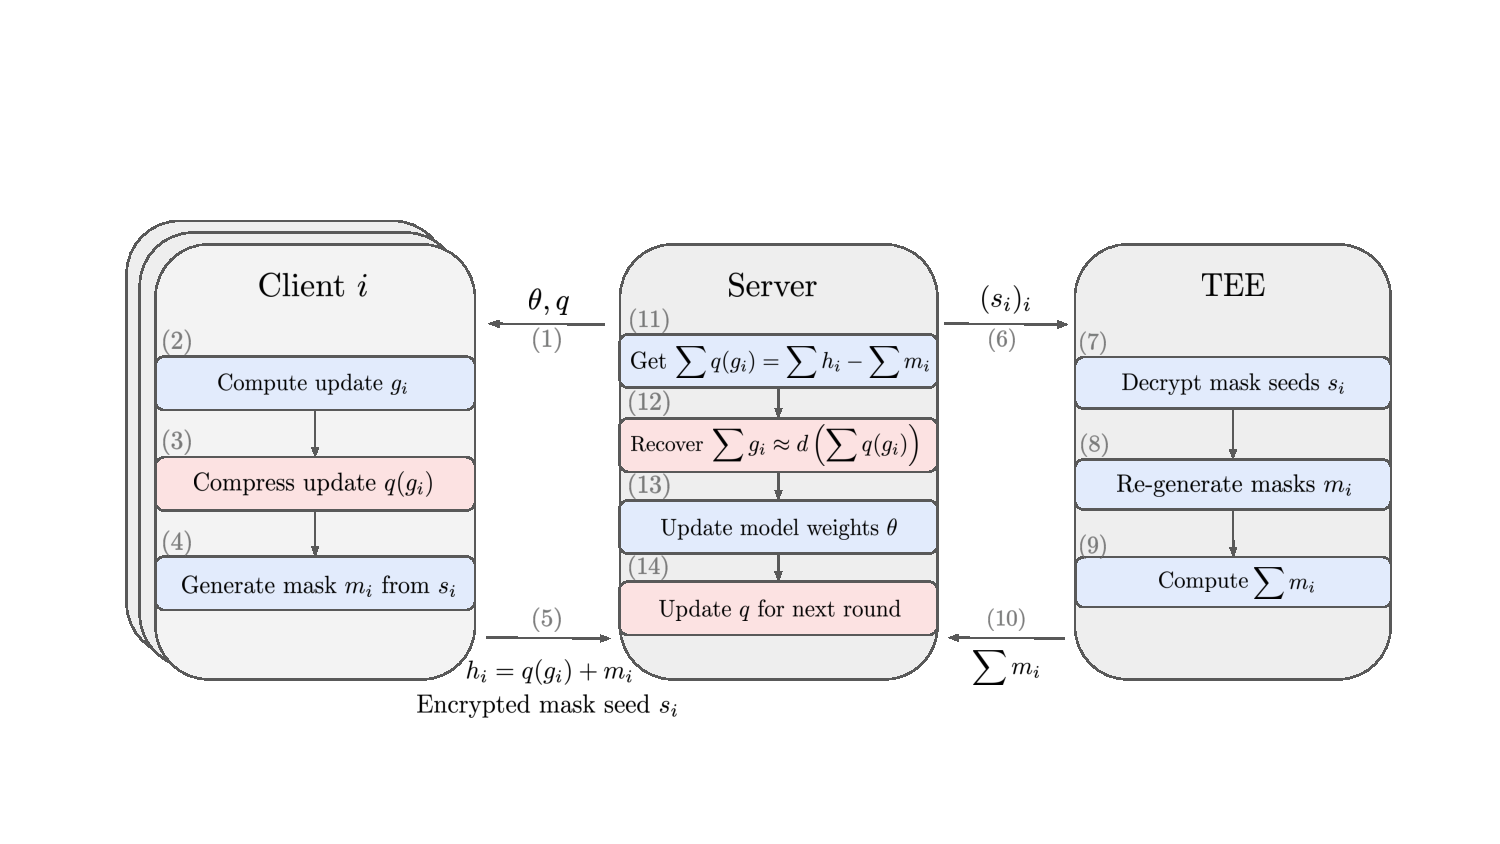
\includegraphics[width=0.8\textwidth]{figs/secagg_summary_new.pdf}
    %\vspace{-5mm}
    \caption{\label{fig:secagg_summary}
    Summary of the proposed approach for one FL round, where we omit the round dependency and \modif{Differential Privacy (DP)} for clarity. Blue boxes denote standard steps and red boxes denote additional steps for uplink compression. Client $i$ computes local model update $g_i$, compresses it with the compression operator $q$, and encrypts it by adding a random mask $m_i$ in the compressed domain, hence reducing the uplink bandwidth (steps 2--4). The server recovers the aggregate in the compressed domain by leveraging any \SecAgg protocol \modif{(steps 7--13, with a TEE-based \SecAgg, see Section~\ref{subsec:secagg})}. Since the decompression operator $d$ is linear, the server can convert the aggregate back to the non-compressed domain, up to compression error (step 12). As with the model weights $\theta$, the compression operator $q$ are also periodically updated and broadcast by the server (step 14). 
    In Section~\ref{sec:method}, we apply the proposed method to scalar quantization and pruning without impacting \SecAgg and propose Secure Indexing, a variant of \SecAgg for extreme uplink compression with product quantization. See Section~\ref{subsec:secagg} for details about \SecAgg and Section~\ref{sec:discussion} for a discussion on~DP.
    }
    \vspace{-3mm}
\end{figure*}



% Our focus in this paper is on 

%Second, scaling cross-device (synchronous) FL to millions of clients with various capabilities and intermittent availability \citep{bonavitz2019federated} suffers from diminishing returns: the wall-clock training time plateaus as the number of clients keeps increasing~\citep{huba2021papaya}. Even though this challenge can be addressed by leveraging the buffered asynchronous aggregation technique proposed by \cite{nguyen2021federated}, compatible with DP and SecAgg, the asynchronous protocol remains bottlenecked by communication latency between the server and the clients.


%Considering the above privacy and scalability goals, we focus on enabling efficient FL communications while keeping a high privacy bar. In addition to the primary objective of speeding up convergence, reducing communication costs brings other significant benefits. Lowering communication requirements addresses selection bias due to undersampling clients with limited connectivity, improving fairness and inclusivity metrics. Better communication efficiency shrinks the carbon footprint of FL, whose fraction attributable to communication can reach 95\%~\citep{qiu2021first}. %Finally, training larger model in FL would be a possibility, when the communication cost is reduced, because local memory or compute requirements can be addressed by modifying the local training loop, for instance with gradient checkpointing \citep{chen2016training}. However, some form of compression would be required to enable efficient communication.


%First, compressing model updates from the client to the server presents several challenges due to compatibility with SecAgg and is an area suitable for further research. 
%Second, upload bandwidth is generally more restricted than download. For instance, according to the most recent FCC report, the ratio of download to upload speeds for DSL/cable providers in the US ranges between 3$\times$ to 20$\times$~\citep{fcc-broadband}. We consider broadband speeds here because devices participate in the FL training while connected to fixed broadband, usually through Wi-Fi~\citep{huba2021papaya}.




% Hence, FL provides the ability to leverage data from massive client populations while ensuring the security and privacy of the client data.
% Go further: compatibility with DP / compression as a mitigation techniques of attacks
% Model and gradient compression intrinsically different.
%  Why not having the secure enclave perform the aggregation?

\section{Related Works}

The first guarantee for FedAvg, showing that it converges at the same rate as mini-batch SGD in strongly convex scenarios, was shown by \cite{stich2018local} in the IID setting. The further convergence analysis of FedAvg for non-convex functions was laid out in a number of published works \cite{wang2018cooperative, haddadpour2019trading, yu2019parallel}. Followup work has managed to remove unnecessary assumptions, such as uniformly bounded gradients, to achieve better convergence rates \cite{wang2018cooperative, stich2019error, haddadpour2019local, khaled2020tighter, woodworth2020local}. Moreover, \cite{li2018federated, haddadpour2019convergence, li2019convergence, khaled2020tighter, karimireddy2020scaffold} define scenarios that depart from the IID framework, analyzing the convergence of FedAvg and its variants in settings with heterogeneous data distributions.

Reducing the transmitted bits between a server and clients through compression techniques is pivotal to saving communication costs in federated learning. This motivates researchers to develop various compression techniques such as sparsification and quantization without significantly sacrificing accuracy \cite{konevcny2016federated, alistarh2017qsgd, suresh2017distributed, wangni2017gradient, bernstein2018signsgd, wang2018atomo, vogels2019powersgd, horvath2019natural, basu2019qsparse, rothchild2020fetchsgd}. \cite{reisizadeh2020fedpaq} show near-optimal theoretical guarantees of the first federated optimization algorithm that incorporates federated averaging, partial node participation, and quantization in homogeneous local data distribution settings. \cite{haddadpour2021federated} further provide improved convergence rates for both homogeneous and heterogeneous settings.

We can achieve better communication efficiency by applying acceleration methods into client updates. \cite{yuan2020federated} have proposed the first provable acceleration of FedAvg that achieves a linear speedup with the fewest communication rounds. Several other works aim to achieve communication efficiency by using momentum or adaptive optimizers \cite{yu2019linear, karimireddy2020mime, wang2021local}. It is important to note that our work is not the first to combine acceleration and quantization.  \cite{li2020acceleration, li2021canita}, for example, propose compressed and accelerated distributed optimization methods that are neither stochastic nor FedAvg variants. \cite{singh2021squarm} propose communication efficient momentum SGD for decentralized optimization. \cite{li2022distributed, wang2022communication} show that distributed and federated versions of adaptive optimizers along with gradient compression can lead to similar convergence rates as their non-compressed counterparts. But these works do not achieve the core result of the present paper, which is the reduced communication complexity via a faster convergence rate and a linear speedup with the small number of communication rounds. To the best of our knowledge, FedAQ is the first accelerated version of federated averaging for master-worker topology that successfully integrates a quantization scheme and provides rigorous convergence guarantees. 

\section{Problem Setup} \label{problem_setup}

In this paper, we build our algorithm based on federated learning with captain-worker topology where $M$ local devices contain their own local data, and a server aggregates local parameter updates without sharing any data during synchronization rounds. Since we focus on \emph{homogeneous} local data distribution settings for the convergence analysis of our algorithm, we define the distributed stochastic optimization problem as below.
\begin{align*}
    \min_{w \in \mathbb{R}^d} F(w) := \mathbb{E}_{z\sim\mathcal{D}}[f(w;z)]
\end{align*}
In our convergence analysis, we assume $F$ is \emph{strongly-convex}. Each client can access $F$ at $w$ via oracle $\nabla f(w;z)$ because all clients have the same loss function $f$. Also, every local device has the same local data distribution $\mathcal{D}$. Moreover, we use the \emph{full participation} of nodes for local updates and synchronizations.

\subsection{Assumptions}

Let us clarify assumptions on the unbiased quantizer $Q$, the global objective function $F$, and the unbiased gradient estimator $\nabla f$.

\begin{assumption} \label{assumption1}
The variance of the unbiased quantizer $Q$ is bounded by the squared of $l_2$-norm of its argument, i.e., $\mathbb{E}[Q(x)|x]=x, \textrm{ } \mathbb{E}[\|Q(x) - x\|^2 |x] \leq q \|x\|^2$.
\end{assumption}
For example, a well-known randomized quantizer which satisfies Assumption \ref{assumption1} is low-precision quantizer in \cite {alistarh2017qsgd}.

\textbf{Example 1.} (Low-precision quantizer) Given $x \in \mathbb{R}^d$, the quantizer $Q:\mathbb{R}^d \rightarrow \mathbb{R}^d$ is defined by
\begin{align*}
    Q_i(x) = \textrm{sign}(x_i)\cdot\|x\|\cdot \xi_i(x, s),   \textrm{ } \textrm{ } i \in [d]
\end{align*}
$\xi_i$ is defined as below.
$$\xi_i(x, s)=
\begin{cases}
\frac{l+1}{s},~\textrm{with probability } \frac{|x_i|}{\|x\|}s - l\\
\frac{l}{s},~\textrm{ } \textrm{ } \textrm{ o/w}
\end{cases}$$
$s$ is the number of quantization levels. $l \in [0, s)$ is an integer which satisfies $\frac{|x_i|}{\|x\|} \in [\frac{l}{s}, \frac{l+1}{s})$.

\begin{assumption} \label{assumption2}
F is $\mu$-strongly convex, i.e., $F(w_1) \geq F(w_2) + \langle \nabla F(w_2), w_1-w_2 \rangle + \frac{1}{2}\mu \|w_1-w_2\|^2$ for any $w_1, w_2 \in \mathbb{R}^d$.
\end{assumption}

\begin{assumption} \label{assumption3}
F is L-smooth, i.e., $F(w_1) \leq F(w_2) + \langle \nabla F(w_2), w_1-w_2 \rangle + \frac{1}{2}L \|w_1-w_2\|^2$ for any $w_1, w_2 \in \mathbb{R}^d$.
\end{assumption}

\begin{assumption} \label{assumption4}
$\nabla f(w; \xi)$ is unbiased and variance bounded, i.e., $\mathbb{E}_\xi[\nabla f(w; \xi)] = \nabla F(w)$, $\mathbb{E}_\xi[\|\nabla f(w; \xi) - \nabla F(w)\|^2] \leq \sigma^2$ for any $w \in \mathbb{R}^d$.
\end{assumption}


\subsection{Notation}

We use $\tau, K$ to respectively denote the number of local updates and total communication rounds, which means the total number of iterations $T$ at each node satisfies $T = K\tau$. Since we consider a strongly-convex case, we can find the optimal point $w^*$ and denote the optimal function value as $F^* := F(w^*)$. The local parameter $w_{k, t}^m$ indicates the parameter of the $m$-th local model after $k$th synchronization followed by $t$ local SGD updates. There are other types of parameters such as $w_{k, t}^{\textrm{ag}, m} \textrm{ and } w_{k, t}^{\textrm{md}, m}$, and we obtain two types of parameters $w_k$ and $w_k^{\textrm{ag}}$ in the server side after $k$th synchronization. More details on these parameters will be discussed in the next section. 

\section{FedAQ Algorithm}

We propose a novel communication efficient algorithm that combines an accelerated variant of federated averaging and an efficient quantization scheme. Our FedAQ algorithm has two main parts: (1) multiple accelerated local updates and (2) communication with quantization. Both components contribute to achieving better communication efficiency than other previous federated algorithms. The entire process is summarized in Algorithm \ref{algorithm1}. %(See Appx.~\ref{app:fedaq_alg}).

\subsection{Multiple Accelerated Local Updates}

The FedAvg algorithm, proposed by \cite{mcmahan2017communication}, is widely used for federated learning to improve communication efficiency by reducing communication rounds with multiple local SGD updates. \cite{yuan2020federated} provide FedAC that replaces the stochastic gradient updates of FedAvg by accelerated version of SGD by \cite{ghadimi2012optimal} resulting in a linear speedup in $M$ with fewer communication rounds than FedAvg.

Thus, we apply the FedAC scheme to multiple updates of each local model. Since previous quantization-based federated optimization algorithms are FedAvg variants with no acceleration, the accelerated method enables our algorithm to gain better communication efficiency than others.

As you can see in Algorithm \ref{algorithm1}, we need two more local parameters $w_{k, t}^{\textrm{ag}, m}$ and $w_{k, t}^{\textrm{md}, m}$ for acceleration in addition to the main local parameter $w_{k, t}^m$. $w_{k,t}^{\textrm{ag},m}$ aggregates the past iterates, and the gradients are queried at the auxiliary parameter $w_{k,t}^{\textrm{md},m}$. While typical FL algorithms without acceleration only have a learning rate $\eta$ as their hyperparameter, the general acceleration scheme makes our algorithm flexible due to four hyperparameters $\alpha, \beta, \eta, \gamma$. $\alpha, \beta$ are hyperparameters related to coupling coefficients, and $\eta, \gamma$ stand for learning rates respectively for $w_{k, t}^{\textrm{ag}, m}, w_{k, t}^m$. The flexibility of hyperparameters enables the fast convergence speed of FedAQ, but naively chosen hyperparameters also cause unstable training of FedAQ. We discuss the exact choice of hyperparameters in \cref{convergence_analysis}. Unlike FedAC, that requires each client to communicate the exact iterates to the server with high precision, we discuss in the following subsection how FedAQ incorporates quantization techniques to reduce communication cost.


%Thus, we carefully determine two parameter condition sets that theoretically ensure the convergence guarantees. The first one is
% \begin{align} \label{parameter_FedAQ}
%     \eta, \gamma \in \Big( 0, \frac{1}{L} \Big], \gamma = \max \Big( \sqrt{\frac{\eta}{\mu\tau}}, \eta \Big), \alpha = \frac{1}{\gamma\mu}, \beta = \alpha + 1
% \end{align}
% We add one more condition $\gamma \in (0, \frac{1}{L}]$ to the FedAC-I condition \cite{yuan2020federated} and create our parameter condition set (\ref{parameter_FedAQ}). The second one is
% \begin{align} \label{parameter2_FedAQ}
%     \eta, \gamma \in \Big( 0, \frac{1}{L} \Big], \gamma = \max \Big( \sqrt{\frac{\eta}{\mu\tau}}, \eta \Big), \alpha=\frac{3}{2\gamma\mu} - \frac{1}{2}, \beta = \frac{2\alpha^2-1}{\alpha-1}, \gamma\mu \leq \frac{3}{4}
% \end{align}
% We add two more conditions $\gamma \in (0, \frac{1}{L}]$ and $\gamma\mu \leq \frac{3}{4}$ to the FedAC-II condition to build our parameter condition set (\ref{parameter2_FedAQ}). Even though quantization adds complexity to the algorithm, these weak assumptions are the only additional requirements for showing the convergence of FedAQ. More details on how the above conditions help the convergence proof of FedAQ are shown in Appx.~\ref{app:proof_lemma} and Appx.~\ref{app:proof_lemma2}.

\subsection{Communication with Quantization}

In cross-device federated learning, a large amount of communicated messages from a number of devices and the limited communication bandwidth can lead to severe communication bottlenecks. Therefore, in this scenario, an efficient quantization scheme can significantly reduce the size of communicated messages and make communication between local devices and a server faster. We apply the same unbiased quantizer used in \cite{haddadpour2021federated} that satisfies Assumption \ref{assumption1}.

In contrast with other quantization-based federated optimization algorithms \cite{reisizadeh2020fedpaq, haddadpour2021federated}, the algorithmic novelty of FedAQ is based on applying quantization to two model parameter updates, which is required in order to simultaneously reduce the frequency of communication and the volume of communicated bits. To the best of our knowledge, this is the first quantization-based method that achieves the accelerated rate with the dramatic reduction in communication cost.
% federated optimization  where quantization is used for two model updates during a synchronization step with theoretical guarantees of how acceleration reduces the number of communication rounds to achieve a linear speedup for quantization-based methods.
To be specific on the communication process, after each client $m$ obtains $w_{k, \tau}^m, w_{k, \tau}^{\textrm{ag}, m}$ through $\tau$ accelerated local iterations, each client quantizes the difference between $w_{k, \tau}^m, w_{k, \tau}^{\textrm{ag}, m}$ and the most recent server models $w_k, w_k^{\textrm{ag}}$. Then, a server aggregates $Q(w_{k, \tau}^m - w_k), Q(w_{k, \tau}^{\textrm{ag}, m} - w_k^{\textrm{ag}})$ from all clients. After dequantizing those messages, the server obtains the following new models $w_{k+1}, w_{k+1}^{\textrm{ag}}$ and broadcasts them back to each client.
% \begin{align*}
%     w_{k+1} &= w_k + \frac{1}{M}\sum_{m=1}^M Q(w_{k, \tau}^m - w_k)\\
%     w_{k+1}^{\textrm{ag}} &= w_k^{\textrm{ag}} + \frac{1}{M} \sum_{m=1}^M Q(w_{k, \tau}^{\textrm{ag}, m} - w_k^{\textrm{ag}})
% \end{align*}

\begin{algorithm} %[H]
\caption{Federated Accelerated SGD with Quantization (FedAQ)}\label{algorithm1}
\begin{algorithmic}[1]
\State{\bfseries Input:} $\alpha, \beta, \eta, \gamma$, initial vector $w_0 = w_{0, 0}^{\textrm{ag}, m} = w_{0, 0}^m$ for all devices $m \in [M]$
\For{$k = 0, \cdots, K-1$}
\For{each client $m$ in parallel}
\State $w_{k, 0}^m \leftarrow w_k, w_{k, 0}^{\textrm{ag}, m} \leftarrow w_k^{\textrm{ag}}$
\For{$t = 0, \cdots, \tau-1$}
\State $w_{k, t}^{\textrm{md}, m} \leftarrow \beta^{-1}w_{k, t}^m + (1-\beta^{-1})w_{k, t}^{\textrm{ag}, m}$
\State $g_{k, t}^m \leftarrow \nabla f(w_{k, t}^{\textrm{md}, m}, \xi_{k, t}^m)$
\State $w_{k, t+1}^{\textrm{ag}, m} \leftarrow w_{k, t}^{\textrm{md}, m} - \eta g_{k, t}^m $
\State $w_{k, t+1}^m \leftarrow (1-\alpha^{-1})w_{k, t}^m + \alpha^{-1} w_{k, t}^{\textrm{md}, m} - \gamma g_{k, t}^m$
\EndFor
\State send $Q(w_{k, \tau}^m - w_k), Q(w_{k, \tau}^{\textrm{ag}, m} - w_k^{\textrm{ag}})$
\EndFor
\State server finds $w_{k+1} \leftarrow w_k + \frac{1}{M}\sum\limits_{m=1}^M Q(w_{k, \tau}^m - w_k), \textrm{ } w_{k+1}^{\textrm{ag}} \leftarrow w_k^{\textrm{ag}} + \frac{1}{M} \sum\limits_{m=1}^M Q(w_{k, \tau}^{\textrm{ag}, m} - w_k^{\textrm{ag}})$
\EndFor

\end{algorithmic}
\end{algorithm} 

\section{Convergence Analysis}
\label{convergence_analysis}

The rigorous theoretical guarantees of reducing communication complexity under strongly-convex and homogeneous assumptions should come first to ensure the significance of FedAQ as one of the standards of communication-efficient federated optimization algorithms. Proving convergence guarantees of FedAQ even under these assumptions requires careful consideration of the approximation error induced by the quantization scheme combined with the convergence analysis of acceleration based methods.
To recall, in FedAQ the server aggregates two quantized local updates $Q(w_{k, \tau}^m - w_k), Q(w_{k, \tau}^{\textrm{ag}, m} - w_k^{\textrm{ag}})$ from all clients (See line 11 in Algorithm \ref{algorithm1}) in each round. If we simply try to generalize the convergence guarantee of FedAC to incorporate the quantization variance costs, the proof techniques from earlier quantization-based methods cannot be directly applied, as we now have two additional quantization error terms that contribute to the overall cost. A significant amount of additional effort is required in order to account for this new quantization error. %The key challenge in bounding the error terms induced by $Q(w_{k, \tau}^m - w_k), Q(w_{k, \tau}^{\textrm{ag}, m} - w_k^{\textrm{ag}})$ is to show that both the local model parameters $w_{k, t}^m$, $w_{k, t}^{\textrm{ag}, m}$ converge to $w^*$ as number of communication rounds and local updates increase.

In this section, we first define two condition sets of hyperparameters used for the convergence analysis of FedAQ. Then, we provide the proof sketch of FedAQ under one such condition set that leads to the better convergence rate $\Tilde{\mathcal{O}}(\frac{1+q}{MT}+\frac{1+q}{TK^3})$. The full proofs of lemmas, theorems, and corollaries under both condition sets are elaborated in \cref{app:proofs} and \cref{app:proofs2}. Finally, we discuss how we obtain the new convergence rate for \cite{haddadpour2021federated} and look into more theoretical details on contribution \ref{contribution2} in Introduction.  %The full proofs of lemmas, theorems, and corollaries are elaborated in Appx.~\ref{app:proofs} and Appx.~\ref{app:proofs2}. %Let us first dive into the proof sketch of FedAQ under the condition set (\ref{parameter_FedAQ}).

\subsection{Two Parameter Condition Sets}

We carefully determine two parameter condition sets that theoretically ensure the convergence guarantees. The first one is
\begin{align} \label{parameter_FedAQ}
    \eta, \gamma \in \Big( 0, \frac{1}{L} \Big], \gamma = \max \Big( \sqrt{\frac{\eta}{\mu\tau}}, \eta \Big), \alpha = \frac{1}{\gamma\mu}, \beta = \alpha + 1
\end{align}
We add one more condition $\gamma \in (0, \frac{1}{L}]$ to the FedAC-I condition \cite{yuan2020federated} and create our parameter condition set (\ref{parameter_FedAQ}). The second one is
\begin{align} \label{parameter2_FedAQ}
    \eta, \gamma \in \Big( 0, \frac{1}{L} \Big], \gamma = \max \Big( \sqrt{\frac{\eta}{\mu\tau}}, \eta \Big), \alpha=\frac{3}{2\gamma\mu} - \frac{1}{2}, \beta = \frac{2\alpha^2-1}{\alpha-1}, \gamma\mu \leq \frac{3}{4}
\end{align}
We add two more conditions $\gamma \in (0, \frac{1}{L}]$ and $\gamma\mu \leq \frac{3}{4}$ to the FedAC-II condition to build our parameter condition set (\ref{parameter2_FedAQ}). Even though quantization adds complexity to the algorithm, these weak assumptions are the only additional requirements for showing the convergence of FedAQ. Moreover, although the better convergence rate $\Tilde{\mathcal{O}}(\frac{1+q}{MT}+\frac{1+q}{TK^3})$ is obtained from the condition set (\ref{parameter2_FedAQ}), we also analyze the convergence of FedAQ under the condition set (\ref{parameter_FedAQ}) because this set empirically leads to more stable training and better performance in experiments than the condition set (\ref{parameter2_FedAQ}) (See Strongly convex case in \cref{qualitative_analysis}). The intuition of the less stable training of FedAQ under the condition set (\ref{parameter2_FedAQ}) comes from larger $\alpha, \beta$ than those of the condition set (\ref{parameter_FedAQ}). If $\alpha, \beta$ are too large, $\alpha^{-1}, \beta^{-1}$ in Algorithm \ref{algorithm1} cannot be used as proper coupling coefficients for local parameters $w_{k, t}^m, w_{k, t}^{\textrm{ag}, m}, w_{k, t}^{\textrm{md}, m}$. This results in aggressive updates and less stable training behavior.

\subsection{Proof Sketch of FedAQ Under Condition Set (\ref{parameter2_FedAQ})}

The decentralized potential $\Phi_{k, t}$ \cite{yuan2020federated} is used for our convergence analysis. People commonly use this potential for acceleration analysis \cite{bansal2019potential}.
\begin{gather*}
    \Phi_{k, t} = F(\Bar{w}_{k, t}^{\textrm{ag}}) -F^* + \frac{1}{6} \mu \|\Bar{w}_{k, t} - w^*\|^2
\end{gather*}
$\Bar{w}_{k, t}$ and $\Bar{w}_{k, t}^{\textrm{ag}}$ is respectively the average of $w_{k, t}^m$ and $w_{k, t}^{\textrm{ag, m}}$ for all $m$. Here, we additionally define $\Phi_k$ as below.
\begin{gather*}
    \Phi_k := \Phi_{k, 0} = F(w_k^{\textrm{ag}}) - F^* + \frac{1}{6} \mu \|w_k - w^*\|^2
\end{gather*}
Since $w_k$ and $w_k^{\textrm{ag}}$ are parameters obtained after $k$th synchronization in a server side, $\Phi_k$ can be considered as the potential of server models. $\Phi_k$ is essential to show the convergence of FedAQ because there is the computation of the quantizer between $\Phi_{k-1, \tau}$ and $\Phi_{k, 0}$. Thus, we should not naively track $\Phi_{k, t}$ but track $\Phi_k$ for our analysis. Obtaining $\Phi_k \leq \epsilon$ would imply that $F(w_k^{\textrm{ag}}) - F^* \leq \epsilon$ and since $F^* \leq F(w_k^{\textrm{ag}})$, it would also imply that $\|w_k - w^*\|^2 = O(\epsilon)$, thus obtaining convergence in terms of both the objective value and the iterate.

Our goal is to show the convergence of FedAQ and derive the simplified convergence rate so that we can get the number of communication rounds to achieve a linear speedup in $M$. As the first step to show this, we prove Lemma \ref{lemmaD.1} which represents the relationship between two consecutive server potential functions $\Phi_k$ and $\Phi_{k+1}$. The quantization scheme amplifies the instability to the convergence of FedAQ in addition to the effect of acceleration. Despite this challenge, we derive Lemma \ref{lemmaD.1} with the help of subtle Propositions (See \cref{app:proof_lemma2}).

% \begin{lemma} \label{lemma3.1}
%  Let F be $\mu$-strongly convex, and assume Assumption \ref{assumption1}, \ref{assumption2}, \ref{assumption3}, \ref{assumption4}, then for $\alpha=\frac{1}{\gamma\mu}, \beta=\alpha+1, \gamma \in [\eta, \sqrt{\frac{\eta}{\mu}}], \eta, \gamma \in (0, \frac{1}{L}], \tau \geq 2, $ FedAQ yields
%  \begin{align*}
%      \mathbb{E}[&\Psi_{k+1}] \leq C(\gamma, \tau) \mathbb{E}[\Psi_k] + \frac{1}{2}(\eta^2 L+\frac{\gamma^2\mu}{M})\tau\sigma^2 \\
%      &+ \gamma\mu L \tau \cdot \max_{0\leq t <\tau} \mathbb{E}[\frac{1}{M} \sum_{m=1}^M \|\Bar{w}_{k, t}^{\textrm{md}} - w_{k, t}^{\textrm{md}, m}\| \|\frac{1}{1+\gamma\mu}(\Bar{w}_{k, t} - w_{k, t}^m) + \frac{\gamma\mu}{1+\gamma\mu}(\Bar{w}_{k, t}^{\textrm{ag}} - w_{k, t}^{\textrm{ag}, m})\|] \\
%      &+ \underbrace{\frac{q}{M}(\gamma^2\mu+\eta^2 L)\tau\sigma^2 + \frac{q}{2M}\Big(\frac{(\gamma-\eta)^2\gamma^2\mu^2(\mu+L)}{(1+\gamma\mu)^2} + \frac{\gamma^4(\mu+L)^2 L}{1+\gamma\mu}\Big)\tau^3\sigma^2}_{\textrm{Additional terms due to quantization}}
%  \end{align*}
%  Where $C(\gamma, \tau)$ is defined as
%  \begin{align*}
%      C(\gamma, \tau) = (1-\gamma\mu)^\tau + \underbrace{\frac{q}{M}\Big( \frac{4\gamma^2\mu(\mu + L)}{(1+\gamma\mu)^2} + \frac{2L\gamma^2(\mu+L)}{1+\gamma\mu}\Big)\tau^2}_{\textrm{Additional terms due to quantization}}
%  \end{align*}
% \end{lemma}

\begin{lemma} \label{lemmaD.1}
 Let F be $\mu$-strongly convex, and assume Assumption \ref{assumption1}, \ref{assumption2}, \ref{assumption3}, \ref{assumption4}, then for $\alpha=\frac{3}{2\gamma\mu} - \frac{1}{2}, \beta=\frac{2\alpha^2-1}{\alpha-1}, \gamma \in [\eta, \sqrt{\frac{\eta}{\mu}}], \eta, \gamma \in (0, \frac{1}{L}], \gamma\mu \leq \frac{3}{4},\tau \geq 2, $ FedAQ yields
 \begin{align*}
     \mathbb{E}[\Phi_{k+1}] &\leq D(\gamma, \tau) \mathbb{E}[\Phi_k] + (\frac{\eta^2 L}{2} + \frac{\gamma^2\mu}{6})\frac{\tau\sigma^2}{M} + \gamma\tau \cdot \max_{0\leq t <\tau} \mathbb{E}[\|\nabla F(\Bar{w}_{k, t}^{\textrm{md}})- \frac{1}{M} \sum_{m=1}^M \nabla F(w_{k, t}^{\textrm{md}, m})\|^2]\\
     &+ \underbrace{\frac{q}{M}(\frac{\gamma^2\mu}{3}+\eta^2 L)\tau\sigma^2 + \frac{q}{2M}\Big( (\gamma-\eta)^2 \gamma^2\mu^2 (\frac{\mu}{3} + \frac{L}{4}) + \gamma^4 (\frac{\mu}{3} + L)^2 L \Big)\tau^3\sigma^2}_{\textrm{additional terms due to quantization}}
 \end{align*}
 Where $D(\gamma, \tau)$ is defined as
 \begin{align*}
     D(\gamma, \tau) &= (1-\frac{1}{3}\gamma\mu)^\tau + \underbrace{\frac{q}{M}\Big( \gamma^2\mu(\frac{8}{3}\mu + 2L) + 2\gamma^2 L(\frac{\mu}{3} + L)\Big)\tau^2}_{\textrm{additional terms due to quantization}}
 \end{align*}
\end{lemma}

We get the inequality between $\Phi_k$ and $\Phi_{k+1}$ by finding the upper bounds of error terms due to multiple($\tau$) local steps and the quantization step. The upper bound of the error caused by multiple local steps is obtained with the help of the analysis in \cite{yuan2020federated} (See Proposition \ref{propositionD.3}). Also, we get the tight upper bound of the error due to quantization with our new proof techniques (See Proposition \ref{propositionD.4}, \ref{propositionD.5}, \ref{propositionD.6}). The key challenge in bounding the quantization error terms comes from representing the upper bound of variances of the quantizer $Q$ on two local updates $w_{k, \tau}^m - w_k, w_{k, \tau}^{\textrm{ag}, m} - w_k^{\textrm{ag}}$ in the form of a server potential $\Phi_k$. Some terms in Lemma \ref{lemmaD.1} are similar to those in Lemma C.2 of the FedAC paper \cite{yuan2020federated}, but our lemma contains additional terms that emerge from the quantization scheme.

For the next step, by telescoping Lemma \ref{lemmaD.1}, we obtain the main theoretical result Theorem \ref{theorem2}. Theorem \ref{theorem2} represents how $\Phi_K$ decreases from the initial potential $\Phi_0$ as a communication round $K$ increases. Since we aim to telescope Lemma \ref{lemmaD.1}, $D(\gamma, \tau)$ should be smaller than 1. Specifically, we show $D(\gamma, \tau) \leq 1-\frac{1}{6}\gamma\mu\tau$ with condition (\ref{condition2}) (See \cref{app:proof_theorem2}). That's why Theorem \ref{theorem2} requires the learning rate $\gamma$ to satisfy the certain condition (\ref{condition2}).

% \begin{theorem} \label{theorem1}
%     Let F be $\mu$-strongly convex, and assume Assumption \ref{assumption1}, \ref{assumption2}, \ref{assumption3}, \ref{assumption4}, then for $\alpha=\frac{1}{\gamma\mu}, \beta=\alpha+1, \gamma = \max(\eta, \sqrt{\frac{\eta}{\mu\tau}}), \eta, \gamma \in (0, \frac{1}{L}], \tau \geq 2, $ if the learning rate $\gamma$ satisfies
%     \begin{align} \label{condition1}
%         \Big(\mu^2 + \frac{q}{M}(\mu+L)(4\mu+2L)\Big)\gamma\tau \leq \frac{1}{2}\mu
%     \end{align}
%     FedAQ yields
%     \begin{align*}
%         &\mathbb{E}[\Psi_K] \leq \exp{\Big(-\frac{1}{2}\max(\eta\mu, \sqrt{\frac{\eta\mu}{\tau}})K\tau\Big)} \Psi_0 + (2q+1)(\frac{\eta^{\frac{1}{2}}\sigma^2}{\mu^{\frac{1}{2}}M\tau^{\frac{1}{2}}} + \frac{\eta\sigma^2}{M}) + 14\eta^2 L\tau\sigma^2 \\
%         &+ \frac{(780+\frac{2q}{M})\eta^{\frac{3}{2}}L\tau^{\frac{1}{2}}\sigma^2}{\mu^{\frac{1}{2}}} + \frac{(\mu+L)(\mu^2+\mu L+L^2)q\eta^{\frac{3}{2}}\tau^{\frac{1}{2}}\sigma^2}{\mu^{\frac{5}{2}}M} + \frac{q\eta^3\tau^2(\mu+L)^2 L\sigma^2}{\mu M}
%     \end{align*}
% \end{theorem}

\begin{theorem} \label{theorem2}
    Let F be $\mu$-strongly convex, and assume Assumption \ref{assumption1}, \ref{assumption2}, \ref{assumption3}, \ref{assumption4}, then for the parameter condition set (\ref{parameter2_FedAQ}), $\tau \geq 2, $ if the learning rate $\gamma$ satisfies
    \begin{align} \label{condition2}
        \bigg( \frac{1}{9}\mu^2 +\frac{q}{M}\Big( \mu(\frac{8}{3}\mu +2L) + 2L(\frac{\mu}{3}+L)\Big)\bigg)\gamma\tau \leq \frac{1}{6}\mu
    \end{align}
    FedAQ yields
    \begin{align*}
        \mathbb{E}[\Phi_K] &\leq \exp{\Big(-\frac{1}{6}\max(\eta\mu, \sqrt{\frac{\eta\mu}{\tau}})K\tau\Big)} \Phi_0 + \frac{2(2q+1)\eta^{\frac{1}{2}}\sigma^2}{\mu^{\frac{1}{2}}M\tau^{\frac{1}{2}}} + \frac{8(q+25)\eta^2 L^2\tau\sigma^2}{\mu} \\
        &+ \frac{3q\Big(\mu^2(\frac{\mu}{3}+\frac{L}{4}) + L(\frac{\mu}{3}+L)^2\Big)\eta^{\frac{3}{2}}\tau^{\frac{1}{2}}\sigma^2}{\mu^{\frac{5}{2}}M} + \frac{3qL(\frac{\mu}{3}+L)^2 \eta^3\tau^2\sigma^2}{\mu M}
    \end{align*}
\end{theorem}

We get the convergence rate of FedAQ with respect to $\eta$ under the condition set (\ref{parameter2_FedAQ}). The final step is to tune $\eta$ appropriately and obtain a more intuitive form of convergence rate that we can easily analyze a linear speedup in $M$. The exact form of this can be found in Corollary \ref{corollary2}. Here, we introduce the simplified form of Corollary \ref{corollary2}.

% \begin{corollary} \label{corollary1}
%     Let $C_1, C_2,\textrm{ and } \eta_0$ as below. Note that $T = K\tau$.
%     \begin{align*}
%         C_1 &= \frac{(\mu+L)(\mu^2+\mu L+L^2)q}{\mu^{\frac{5}{2}}}, \textrm{ } C_2 = \frac{q(\mu+L)^2 L}{\mu} \\
%         \eta_0 &= \frac{4\tau}{\mu T^2}\log^2\Big(e+\min(\frac{\mu M T \Psi_0}{(2q+1)\sigma^2}, \frac{\mu^2 T^3\Psi_0}{L\tau^2\sigma^2}, \frac{\mu^3 M T^3\Psi_0}{(\mu^{\frac{3}{2}}C_1+8C_2)\tau^2\sigma^2}) \Big)
%     \end{align*}
%     Then for $\eta = \min(\frac{1}{L}, \eta_0)$, FedAQ yields
%     \begin{align}
%         &\mathbb{E}[\Psi_K] \leq \min \Big( \exp(-\tfrac{\mu T}{2L}), \exp(-\tfrac{\mu^{\tfrac{1}{2}}T}{2 L^{\tfrac{1}{2}}\tau^{\tfrac{1}{2}}})\Big) \Psi_0 \nonumber \\
%         &+ \tfrac{7(2q+1)\sigma^2}{\mu MT} \log^2 \Big(e+\tfrac{\mu M T \Psi_0}{(2q+1)\sigma^2}\Big) \\
%         &+ \tfrac{(6465+\tfrac{16q}{M})L\tau^2\sigma^2}{\mu^2 T^3}\log^4 \Big(e+ \tfrac{\mu^2 T^3\Psi_0}{L\tau^2\sigma^2}\Big) \\
%         &+ \tfrac{9(\mu^{\tfrac{3}{2}}C_1+8C_2)\tau^2\sigma^2}{\mu^3 M T^3} \log^6 \Big(e + \tfrac{\mu^3 M T^3\Psi_0}{(\mu^{\tfrac{3}{2}}C_1+8C_2)\tau^2\sigma^2}\Big)
%     \end{align}
% \end{corollary}
% \begin{corollary} \label{corollary2}
%     Let $D_1, D_2,\textrm{ and } \eta_0$ as below. Note that $T = K\tau$.
%     \begin{align*}
%         D_1 &= \frac{\Big( \mu^2(\frac{\mu}{3}+\frac{L}{4}) + L(\frac{\mu}{3}+L)^2) \Big)q}{\mu^{\frac{5}{2}}}, \textrm{ } D_2 = \frac{q(\frac{\mu}{3}+L)^2 L}{\mu} \\
%         \eta_0 &= \frac{36\tau}{\mu T^2}\log^2\Big(e+\min(\frac{\mu M T \Phi_0}{(2q+1)\sigma^2}, \frac{\mu^3 T^4\Phi_0}{(q+25)L^2\tau^3\sigma^2}, \frac{\mu^3 M T^3\Phi_0}{(\mu^{\frac{3}{2}}D_1+6^3 D_2)\tau^2\sigma^2}) \Big)
%     \end{align*}
%     Then for $\eta = \min(\frac{1}{L}, \eta_0)$, FedAQ yields
%     \begin{align}
%         \mathbb{E}[\Phi_K] &\leq \min \Big( \exp(-\frac{\mu T}{6L}), \exp(-\frac{\mu^{\frac{1}{2}}T}{6 L^{\frac{1}{2}}\tau^{\frac{1}{2}}})\Big) \Phi_0 \nonumber\\
%         &+ \frac{13(2q+1)\sigma^2}{\mu MT} \log^2 \Big(e+\frac{\mu M T \Phi_0}{(2q+1)\sigma^2}\Big) \\
%         &+ \frac{10369(q+25)L^2\tau^3\sigma^2}{\mu^3 T^4}\log^4 \Big(e+ \frac{\mu^3 T^4\Phi_0}{(q+25)L^2\tau^3\sigma^2}\Big) \\
%         &+ \frac{649(\mu^{\frac{3}{2}}D_1+216D_2)\tau^2\sigma^2}{\mu^3 M T^3} \log^6 \Big(e + \frac{\mu^3 M T^3\Phi_0}{(\mu^{\frac{3}{2}}D_1+216 D_2)\tau^2\sigma^2}\Big)
%     \end{align}
% \end{corollary}
\begin{corollary}
    (Simplified form of Corollary \ref{corollary2}) Note that $T = K\tau$. For $\eta = \min(\frac{1}{L}, \tilde{\Theta} (  \frac{\tau}{\mu T^2} ))$, FedAQ yields
    \begin{align*}
        \mathbb{E}[\Phi_K] &\leq \min \Big( \exp(-\frac{\mu T}{6L}), \exp(-\frac{\mu^{\frac{1}{2}}T}{6 L^{\frac{1}{2}}\tau^{\frac{1}{2}}})\Big) \Phi_0 + \Tilde{\mathcal{O}}( \underbrace{\frac{(1+q)\sigma^2}{\mu MT}}_{\textrm{I}} + \underbrace{\frac{(1+q)L^2\tau^3\sigma^2}{\mu^3 T^4}}_{\textrm{II}} + \underbrace{\frac{qL^3 \tau^2 \sigma^2}{\mu^4 M T^3}}_{\textrm{III}})
    \end{align*}
\end{corollary}

The convergence rate of FedAQ under the condition set (\ref{parameter_FedAQ}) is obtained in a similar way. The convergence analysis under the condition set (\ref{parameter_FedAQ}) is elaborated as Lemma \ref{lemma3.1}, Theorem \ref{theorem1}, and Corollary \ref{corollary1} in \cref{app:proofs}.

\begin{remark} \label{remark5.4} The above convergence rate is worse than the convergence rate of FedAC-II according to Theorem C.13 in \cite{yuan2020federated} because there are additive terms related to the quantization noise $q$ in our case. Let's figure out the dominant terms with $\Tilde{\mathcal{O}}$ notation from the above convergence rate. Here, we replace $\tau$ with $\frac{T}{K}$. At first, we can ignore the first term because it decreases exponentially. The second term I would be $\Tilde{\mathcal{O}}(\frac{1+q}{MT})$. Then, the third term II becomes $\Tilde{\mathcal{O}}(\frac{(1+q)\tau^3}{T^4}) = \Tilde{\mathcal{O}}(\frac{1+q}{TK^3})$. Finally, the last term III turns into $\Tilde{\mathcal{O}}(\frac{q\tau^2}{MT^3}) = \Tilde{\mathcal{O}}(\frac{q}{MTK^2})$. Thus, the overall convergence rate of FedAQ under the condition set (\ref{parameter2_FedAQ}) would be $\Tilde{\mathcal{O}}(\frac{1+q}{MT} + \frac{1+q}{TK^3})$. Similarly, we obtain the simplified convergence rate of FedAQ under the condition set (\ref{parameter_FedAQ}) from three terms (14), (15), (16) of Corollary \ref{corollary1}. In this case, the convergence rate of FedAQ is $\Tilde{\mathcal{O}}(\frac{1+q}{MT} + \frac{1}{TK^2})$, and the required number of communication rounds to achieve a linear speedup in $M$ is $\Tilde{\mathcal{O}}((\frac{M}{1+q})^{\frac{1}{2}})$. \end{remark}

\begin{remark} \label{remark5.5} As we mention above, FedAQ converges at rate $\Tilde{\mathcal{O}}(\frac{1+q}{MT} + \frac{1+q}{TK^3})$, which is better than the convergence rate of \cite{haddadpour2021federated} $\Tilde{\mathcal{O}}(\frac{1+q}{MT}+\frac{1}{TK})$. To our knowledge, \cite{haddadpour2021federated} obtain the best convergence rate among previous quantization-based federated optimization algorithms. Actually, in the strongly-convex and homogeneous case, \cite{haddadpour2021federated} provide different convergence rate $\mathcal{O}(\frac{1}{\gamma^2\tau} + \frac{(q+1)}{(\frac{q}{M}+1)\tau M}) = \mathcal{O}(\frac{K}{\gamma^2 T} + \frac{(q+1)K}{(\frac{q}{M}+1)T M})$, where $\gamma$ is a learning rate for the server updates. They achieve this convergence rate by tuning $\eta = \frac{1}{2L(\frac{q}{M} + 1)\tau \gamma}$. However, we cannot say this algorithm achieves a linear speedup in this scenario. That's why we provide a new convergence rate $\Tilde{\mathcal{O}}(\frac{1+q}{MT}+\frac{1}{TK})$ for \cite{haddadpour2021federated} by tuning $\eta$ in a different way. This new $\eta$ makes this algorithm achieve a linear speedup. Why the original $\eta$ cannot achieve a linear speedup and how we get new $\eta$ can be found in \cref{app:fedcomgate}.
\end{remark}

\subsection{Proof Details for FedAQ under Condition Set (\ref{parameter_FedAQ})}
\label{app:proofs}

Before diving into proof details, we define $\Bar{w}_{k, \tau}, \Bar{w}_{k, \tau}^{\textrm{ag}}, \Psi_{k, t}^m, \Psi_{k, t}, \Psi_k, A_{k, t}^m$ as below.
\begin{align*}
    \Bar{w}_{k, \tau} &= \frac{1}{M} \sum_{m=1}^M w_{k, \tau}^m \\
    \Bar{w}_{k, \tau}^{\textrm{ag}} &= \frac{1}{M} \sum_{m=1}^M w_{k, \tau}^{\textrm{ag}, m} \\
    \Psi_{k, t}^m &= F(w_{k, t}^{\textrm{ag}, m}) - F^* + \frac{1}{2} \mu \|w_{k, t}^m - w^*\|^2\\
    \Psi_{k, t} &= \frac{1}{M} \sum_{m=1}^M F(w_{k, t}^{\textrm{ag}, m}) -F^* + \frac{1}{2} \mu \|\Bar{w}_{k, t} - w^*\|^2 \\
    \Psi_k :&= \Psi_{k, 0} = F(w_k^{\textrm{ag}}) - F^* + \frac{1}{2} \mu \|w_k - w^*\|^2\\
    A_{k, t}^m &= \frac{\gamma^2\mu^2 (\mu+L)}{(1+\gamma\mu)^2}\|w_{k, t}^m - w_{k, t}^{\textrm{ag}, m}\|^2 + \gamma^2(\mu + L)\frac{2L}{1+\gamma\mu}\Psi_{k, t}^m
    %\chi_{k, t}^m &= \frac{\mu}{2}\|w_{k, t}^m - w_k\|^2 + \frac{L}{2} \|w_{k, t}^{\textrm{ag}, m} - w_k^{\textrm{ag}}\|^2
\end{align*}
The above notations are essential to our convergence analysis. Intuitively, if the FedAQ algorithm converges to the optimal point, $\Bar{w}_{k, \tau}, \Bar{w}_{k, \tau}^{\textrm{ag}}$ become $w^*$, and $\Psi_{k, t}^m, \Psi_{k, t}, \Psi_k, A_{k, t}^m$ become 0. In order to denote the $\sigma$-algebra generated by $\{w_{k^\prime, t^\prime}^m, w_{k^\prime, t^\prime}^{\textrm{ag}, m}\}_{(k^\prime < k) \textrm{ or } (k^\prime = k, t^\prime \leq t), m \in [M]}$, we use $\mathcal{F}_{k, t}$.

\subsubsection{Proof of Lemma \ref{lemma3.1}}
\label{app:proof_lemma}

\begin{lemma} \label{lemma3.1}
 Let F be $\mu$-strongly convex, and assume Assumption \ref{assumption1}, \ref{assumption2}, \ref{assumption3}, \ref{assumption4}, then for $\alpha=\frac{1}{\gamma\mu}, \beta=\alpha+1, \gamma \in [\eta, \sqrt{\frac{\eta}{\mu}}], \eta, \gamma \in (0, \frac{1}{L}], \tau \geq 2, $ FedAQ yields
 \begin{align*}
     \mathbb{E}[&\Psi_{k+1}] \leq C(\gamma, \tau) \mathbb{E}[\Psi_k] + \frac{1}{2}(\eta^2 L+\frac{\gamma^2\mu}{M})\tau\sigma^2 \\
     &+ \gamma\mu L \tau \cdot \max_{0\leq t <\tau} \mathbb{E}[\frac{1}{M} \sum_{m=1}^M \|\Bar{w}_{k, t}^{\textrm{md}} - w_{k, t}^{\textrm{md}, m}\| \|\frac{1}{1+\gamma\mu}(\Bar{w}_{k, t} - w_{k, t}^m) + \frac{\gamma\mu}{1+\gamma\mu}(\Bar{w}_{k, t}^{\textrm{ag}} - w_{k, t}^{\textrm{ag}, m})\|] \\
     &+ \underbrace{\frac{q}{M}(\gamma^2\mu+\eta^2 L)\tau\sigma^2 + \frac{q}{2M}\Big(\frac{(\gamma-\eta)^2\gamma^2\mu^2(\mu+L)}{(1+\gamma\mu)^2} + \frac{\gamma^4(\mu+L)^2 L}{1+\gamma\mu}\Big)\tau^3\sigma^2}_{\textrm{Additional terms due to quantization}}
 \end{align*}
 Where $C(\gamma, \tau)$ is defined as
 \begin{align*}
     C(\gamma, \tau) = (1-\gamma\mu)^\tau + \underbrace{\frac{q}{M}\Big( \frac{4\gamma^2\mu(\mu + L)}{(1+\gamma\mu)^2} + \frac{2L\gamma^2(\mu+L)}{1+\gamma\mu}\Big)\tau^2}_{\textrm{Additional terms due to quantization}}
 \end{align*}
\end{lemma}


In this section, we first introduce five crucial Propositions for proving Lemma \ref{lemma3.1}. Then, we prove Lemma \ref{lemma3.1} by using Propositions in the last part of this section.
\begin{proposition} \label{proposition3.2}
Let Assumption \ref{assumption1} hold and consider any $k$ synchronization round. Then, we can decompose the expectation as follows:
\begin{align*}
    \mathbb{E}[\|w_{k+1} - w^*\|^2] &= \mathbb{E}[\|w_{k+1} - \Bar{w}_{k, \tau}\|^2] + \mathbb{E}[\|\Bar{w}_{k, \tau} - w^*\|^2] \\
    \mathbb{E}[F(w_{k+1}^{\textrm{ag}}) - F^*] &= \mathbb{E}[F(w_{k+1}^{\textrm{ag}}) - \frac{1}{M} \sum_{m=1}^M F(w_{k, \tau}^{\textrm{ag}, m})] + \mathbb{E}[\frac{1}{M} \sum_{m=1}^M F(w_{k, \tau}^{\textrm{ag}, m}) - F^*]
\end{align*}
\end{proposition}

\emph{Proof of Proposition \ref{proposition3.2}} \textrm{ } The second equality is trivial. Let's focus on the first equality. By Assumption \ref{assumption1}, the quantizer $Q$ is unbiased and we get,
\begin{align*}
    \mathbb{E}_Q[w_{k+1}] &= w_k + \frac{1}{M}\sum_{m=1}^M \mathbb{E}_Q Q(w_{k, \tau}^m - w_k) = \frac{1}{M} \sum_{m=1}^M w_{k, \tau}^m = \Bar{w}_{k, \tau}
\end{align*}
Thus, we finally obtain
\begin{align*}
    \mathbb{E}[\|w_{k+1} - w^*\|^2] &= \mathbb{E}[\|w_{k+1} - \Bar{w}_{k, \tau} + \Bar{w}_{k, \tau} - w^*\|^2] \\
    &= \mathbb{E}[\|w_{k+1} - \Bar{w}_{k, \tau}\|^2] + \mathbb{E}[\|\Bar{w}_{k, \tau} - w^*\|^2]
\end{align*}

\begin{proposition} \label{proposition3.3}
Let F be $\mu$-strongly convex, and assume Assumption \ref{assumption2}, \ref{assumption3}, \ref{assumption4}, then for $\alpha=\frac{1}{\gamma\mu}, \beta=\alpha+1, \gamma \in [\eta, \sqrt{\frac{\eta}{\mu}}], \eta \in (0, \frac{1}{L}]$, FedAQ yields
\begin{align*}
    \mathbb{E}[\Psi_{k, \tau}] &\leq (1-\gamma\mu)^\tau \mathbb{E}[\Psi_k] + \frac{1}{2}(\eta^2 L + \frac{\gamma^2\mu}{M})\tau\sigma^2 + \gamma\mu L \tau \\
    &\cdot \max_{0\leq t <\tau} \mathbb{E}[\frac{1}{M} \sum_{m=1}^M \|\Bar{w}_{k, t}^{\textrm{md}} - w_{k, t}^{\textrm{md}, m}\|\|\frac{1}{1+\gamma\mu}(\Bar{w}_{k, t} - w_{k, t}^m) + \frac{\gamma\mu}{1+\gamma\mu}(\Bar{w}_{k, t}^{\textrm{ag}} - w_{k, t}^{\textrm{ag}, m})\|]
\end{align*}
\end{proposition}

\emph{Proof of Proposition \ref{proposition3.3}} \textrm{ } We refer to the proof of Lemma B.2 in \cite{yuan2020federated}. There is no quantization between $\Psi_{k, \tau}$ and $\Psi_k$. Thus, we can directly apply useful inequalities in the proof of Lemma B.2 in \cite{yuan2020federated} to our proof. Then, we obtain
\begin{align*}
    \mathbb{E}[\Psi_{k, t+1}|\mathcal{F}_{k, t}] &\leq (1-\gamma\mu) \Psi_{k, t} + \frac{1}{2}(\eta^2 L + \frac{\gamma^2\mu}{M})\sigma^2 + \gamma\mu L \\
    &\cdot \frac{1}{M} \sum_{m=1}^M \|\Bar{w}_{k, t}^{\textrm{md}} - w_{k, t}^{\textrm{md}, m}\|\|\frac{1}{1+\gamma\mu}(\Bar{w}_{k, t} - w_{k, t}^m) + \frac{\gamma\mu}{1+\gamma\mu}(\Bar{w}_{k, t}^{\textrm{ag}} - w_{k, t}^{\textrm{ag}, m})\|
\end{align*}
From the above relationship between $\Psi_{k, t+1}$ and $\Psi_{k, t}$, we get
\begin{align*}
    \mathbb{E}[\Psi_{k, \tau}] &\leq (1-\gamma\mu)^\tau \mathbb{E}[\Psi_k] + \Big(\sum_{t=0}^{\tau-1} (1-\gamma\mu)^t \Big)\frac{1}{2}(\eta^2 L + \frac{\gamma^2\mu}{M})\sigma^2 + \gamma\mu L \cdot \sum_{t=0}^{\tau-1} \Big\{ (1-\gamma\mu)^{\tau-t-1} \\
    &\mathbb{E}[\frac{1}{M} \sum_{m=1}^M \|\Bar{w}_{k, t}^{\textrm{md}} - w_{k, t}^{\textrm{md}, m}\|\|\frac{1}{1+\gamma\mu}(\Bar{w}_{k, t} - w_{k, t}^m) + \frac{\gamma\mu}{1+\gamma\mu}(\Bar{w}_{k, t}^{\textrm{ag}} - w_{k, t}^{\textrm{ag}, m})\|]\Big\} \\
    &\leq (1-\gamma\mu)^\tau \mathbb{E}[\Psi_k] + \frac{1}{2}(\eta^2 L + \frac{\gamma^2\mu}{M})\tau\sigma^2 + \gamma\mu L \tau \\
    &\cdot \max_{0\leq t <\tau} \mathbb{E}[\frac{1}{M} \sum_{m=1}^M \|\Bar{w}_{k, t}^{\textrm{md}} - w_{k, t}^{\textrm{md}, m}\|\|\frac{1}{1+\gamma\mu}(\Bar{w}_{k, t} - w_{k, t}^m) + \frac{\gamma\mu}{1+\gamma\mu}(\Bar{w}_{k, t}^{\textrm{ag}} - w_{k, t}^{\textrm{ag}, m})\|]
\end{align*}

\begin{proposition} \label{proposition3.4}
Let Assumption \ref{assumption1} hold. Then, we have
\begin{align*}
    \mathbb{E}[\|w_{k+1} - \Bar{w}_{k, \tau}\|^2] &\leq \frac{q}{M^2}\sum_{m=1}^M \mathbb{E}[\|w_{k, \tau}^m - w_k\|^2] \\
    \mathbb{E}[F(w_{k+1}^{\textrm{ag}}) - \frac{1}{M} \sum_{m=1}^M F(w_{k, \tau}^{\textrm{ag}, m})] &\leq \frac{qL}{2M^2} \sum_{m=1}^M \mathbb{E}[\|w_{k, \tau}^{\textrm{ag}, m} - w_k^{\textrm{ag}}\|^2]
\end{align*}
\end{proposition}

\emph{Proof of Proposition \ref{proposition3.4}} \textrm{ } First, let's consider the first inequality. According to Assumption \ref{assumption1}, we get
\begin{align*}
    \mathbb{E}[\|w_{k+1} - \Bar{w}_{k, \tau}\|^2] &= \mathbb{E}[\|w_k + \frac{1}{M} \sum_{m=1}^M Q(w_{k, \tau}^m - w_k) - \frac{1}{M} \sum_{m=1}^M w_{k, \tau}^m\|^2] \\
    &= \mathbb{E}[\|\frac{1}{M} \sum_{m=1}^M Q(w_{k, \tau}^m - w_k) - (w_{k, \tau}^m - w_k)\|^2] \\
    &= \frac{1}{M^2} \sum_{m=1}^M \mathbb{E}[\|Q(w_{k, \tau}^m - w_k) - (w_{k, \tau}^m -w_k)\|^2] \leq \frac{q}{M^2} \sum_{m=1}^M \mathbb{E} \|w_{k, \tau}^m - w_k\|^2
\end{align*}
The third equality comes from the unbiasedness of $Q$, and the last inequality stems from the variance assumption of $Q$. Similarly, we obtain

\begin{align*}
    \mathbb{E}[F(w_{k+1}^{\textrm{ag}}) - \frac{1}{M} \sum_{m=1}^M F(w_{k, \tau}^{\textrm{ag}, m})] &= \mathbb{E}[F(w_k^{\textrm{ag}} + \frac{1}{M}\sum_{m=1}^M Q(w_{k, \tau}^{\textrm{ag}, m} - w_k^{\textrm{ag}})) - \frac{1}{M} \sum_{m=1}^M F(w_{k, \tau}^{\textrm{ag}, m})] \\
    &= \mathbb{E}[\frac{1}{M} \sum_{m=1}^M F(w_k^{\textrm{ag}} + \frac{1}{M}\sum_{m=1}^M Q(w_{k, \tau}^{\textrm{ag}, m} - w_k^{\textrm{ag}})) - F(w_{k, \tau}^{\textrm{ag}, m})] \\
    &\leq \mathbb{E}\Big[\frac{1}{M} \sum_{m=1}^M \langle \nabla F(w_{k, \tau}^{\textrm{ag}, m}), \frac{1}{M} \sum_{m=1}^M \Big( Q(w_{k, \tau}^{\textrm{ag}, m} - w_k^{\textrm{ag}}) - (w_{k, \tau}^{\textrm{ag}, m} \\
    &- w_k^{\textrm{ag}})\Big) \rangle + \frac{L}{2} \|\frac{1}{M} \sum_{m=1}^M  Q(w_{k, \tau}^{\textrm{ag}, m} - w_k^{\textrm{ag}}) - (w_{k, \tau}^{\textrm{ag}, m} - w_k^{\textrm{ag}})\|^2\Big] \\
    &= \frac{L}{2} \mathbb{E}[\|\frac{1}{M} \sum_{m=1}^M  Q(w_{k, \tau}^{\textrm{ag}, m} - w_k^{\textrm{ag}}) - (w_{k, \tau}^{\textrm{ag}, m} - w_k^{\textrm{ag}})\|^2] \\
    &= \frac{L}{2M^2}\sum_{m=1}^M \mathbb{E}[\| Q(w_{k, \tau}^{\textrm{ag}, m} - w_k^{\textrm{ag}}) - (w_{k, \tau}^{\textrm{ag}, m} - w_k^{\textrm{ag}})\|^2] \\
    &\leq \frac{qL}{2M^2} \sum_{m=1}^M \mathbb{E}[\|w_{k, \tau}^{\textrm{ag}, m} - w_k^{\textrm{ag}}\|^2]
\end{align*}

\begin{proposition} \label{proposition3.5}
Let F be $\mu$-strongly convex, and assume Assumption \ref{assumption2}, \ref{assumption3}, \ref{assumption4}, then for $\alpha=\frac{1}{\gamma\mu}, \beta=\alpha+1, \gamma \in [\eta, \sqrt{\frac{\eta}{\mu}}], \eta, \gamma \in (0, \frac{1}{L}], $ we get
\begin{align*}
    \mathbb{E}[A_{k, t}^m] \leq \mathbb{E}[A_{k, 0}^m] + \Big( \frac{(\gamma-\eta)^2(\mu+L)}{1+\gamma\mu}+\frac{\gamma^2(\mu+L)^2 L}{\mu^2}\Big)\cdot \Big( 1-(1-\gamma\mu+\frac{\gamma\mu}{1+\gamma\mu})^t\Big)\sigma^2
\end{align*}
\end{proposition}

\emph{Proof of Proposition \ref{proposition3.5}}
\textrm{ } From the notation mentioned in the beginning of \cref{app:proofs},
\begin{align} \label{eq3.5-1}
    \mathbb{E}[A_{k, t+1}^m|\mathcal{F}_{k, t}] &= \frac{\gamma^2\mu^2 (\mu+L)}{(1+\gamma\mu)^2}\mathbb{E}[\|w_{k, t+1}^m - w_{k, t+1}^{\textrm{ag}, m}\|^2|\mathcal{F}_{k, t}] + \gamma^2(\mu+L)\frac{2L}{1+\gamma\mu}\mathbb{E}[\Psi_{k, t+1}^m|\mathcal{F}_{k, t}]
\end{align}
Thus, let's sequentially compute $\mathbb{E}[\|w_{k, t+1}^m - w_{k, t+1}^{\textrm{ag}, m}\|^2|\mathcal{F}_{k, t}]$ and $\mathbb{E}[\Psi_{k, t+1}^m|\mathcal{F}_{k, t}]$.
\begin{align*}
    \mathbb{E}[\|w_{k, t+1}^m - w_{k, t+1}^{\textrm{ag}, m}\|^2|\mathcal{F}_{k, t}] &= \mathbb{E}[\|(1-\alpha^{-1})w_{k, t}^m + \alpha^{-1}w_{k, t}^{\textrm{md}, m} - \gamma g_{k, t}^m - w_{k, t}^{\textrm{md}, m} + \eta g_{k, t}^m\|^2|\mathcal{F}_{k, t}] \\
    &= \mathbb{E}[\|(1-\alpha^{-1})(w_{k, t}^m - w_{k, t}^{\textrm{md}, m}) - (\gamma-\eta)g_{k, t}^m\|^2|\mathcal{F}_{k, t}] \textrm{ } (\leftarrow \gamma \geq \eta) \\
    &= \|(1-\alpha^{-1})(w_{k, t}^m - w_{k, t}^{\textrm{md}, m}) - (\gamma-\eta)\nabla F(w_{k, t}^{\textrm{md}, m})\|^2 \\
    &+ (\gamma - \eta)^2\mathbb{E}[\|\nabla F(w_{k, t}^{\textrm{md}, m}) - g_{k, t}^m\|^2|\mathcal{F}_{k, t}] \\
    &\leq (1-\alpha^{-1})^2 \|w_{k, t}^m - w_{k, t}^{\textrm{md}, m}\|^2 + (\gamma-\eta)^2 \|\nabla F(w_{k, t}^{\textrm{md}, m})\|^2 \\
    &+ (\gamma-\eta)^2 \sigma^2 - 2(\gamma-\eta) \langle (1-\alpha^{-1})(w_{k, t}^m - w_{k, t}^{\textrm{md}, m}), \nabla F(w_{k, t}^{\textrm{md}, m})\rangle \\
    &\leq (1-\alpha^{-1})^2(1+\gamma\mu) \|w_{k, t}^m - w_{k, t}^{\textrm{md}, m}\|^2 \\
    &+ (\gamma-\eta)^2(1+\frac{1}{\gamma\mu}) \|\nabla F(w_{k, t}^{\textrm{md}, m})\|^2 + (\gamma-\eta)^2 \sigma^2 \\
    &= \frac{(1-\gamma\mu)^2}{1+\gamma\mu}\|w_{k, t}^m - w_{k, t}^{\textrm{ag}, m}\|^2 + (\gamma-\eta)^2\frac{1+\gamma\mu}{\gamma\mu}\|\nabla F(w_{k, t}^{\textrm{md}, m})\|^2 + (\gamma-\eta)^2\sigma^2
\end{align*}
Here, we need to bound $\|\nabla F(w_{k, t}^{\textrm{md}, m})\|^2$.
\begin{align} \label{ineq3.5-2}
    \|\nabla F(w_{k, t}^{\textrm{md}, m})\|^2 &\leq 2L(F(w_{k, t}^{\textrm{md}, m}) - F^*) \textrm{ }(\because \textrm{ Assumption \ref{assumption3}}) \nonumber\\
    &\leq 2L\Big(\beta^{-1}(F(w_{k, t}^m)-F(w^*))+(1-\beta^{-1})(F(w_{k, t}^{\textrm{ag}, m})-F^*)\Big) \nonumber\\
    &\leq \beta^{-1}L^2 \|w_{k, t}^m - w^*\|^2 + 2(1-\beta^{-1})L(F(w_{k, t}^{\textrm{ag}, m})-F^*) \nonumber\\
    &= \frac{\gamma\mu L^2}{1+\gamma\mu}\|w_{k, t}^m - w^*\|^2 + \frac{2L}{1+\gamma\mu}(F(w_{k, t}^{\textrm{ag}, m})-F^*) \nonumber\\
    &\leq \frac{\mu L}{1+\gamma\mu}\|w_{k, t}^m - w^*\|^2 + \frac{2L}{1+\gamma\mu}(F(w_{k, t}^{\textrm{ag}, m})-F^*) = \frac{2L}{1+\gamma\mu}\Psi_{k, t}^m
\end{align}
The last inequality comes from the fact $\gamma \in [0, \frac{1}{L})$. Therefore, we finally get
\begin{align} \label{ineq3.5-3}
    \mathbb{E}[\|w_{k, t+1}^m - w_{k, t+1}^{\textrm{ag}, m}\|^2|\mathcal{F}_{k, t}] &\leq \frac{(1-\gamma\mu)^2}{1+\gamma\mu}\|w_{k, t}^m - w_{k, t}^{\textrm{ag}, m}\|^2 + (\gamma-\eta)^2\frac{1+\gamma\mu}{\gamma\mu}\|\nabla F(w_{k, t}^{\textrm{md}, m})\|^2 + (\gamma-\eta)^2\sigma^2 \nonumber\\
    &\leq \frac{(1-\gamma\mu)^2}{1+\gamma\mu}\|w_{k, t}^m - w_{k, t}^{\textrm{ag}, m}\|^2 + (\gamma-\eta)^2\frac{1+\gamma\mu}{\gamma\mu}\Big(\frac{2L}{1+\gamma\mu}\Psi_{k, t}^m\Big) + (\gamma-\eta)^2\sigma^2
\end{align}
Now, let's compute $\mathbb{E}[\Psi_{k, t+1}^m|\mathcal{F}_{k, t}]$. We need to compute $\mathbb{E}[\|w_{k, t+1}^m-w^*\|^2|\mathcal{F}_{k, t}]$ and $\mathbb{E}[F(w_{k, t+1}^{\textrm{ag}, m}) - F^*|\mathcal{F}_{k, t}]$ first.
\begin{align*}
    \mathbb{E}[\|w_{k, t+1}^m-w^*\|^2|\mathcal{F}_{k, t}] &= \mathbb{E}[\|(1-\alpha^{-1})w_{k, t}^m + \alpha^{-1}w_{k, t}^{\textrm{md}, m} - \gamma g_{k, t}^m -w^*\|^2|\mathcal{F}_{k, t}] \\
    &\leq \|(1-\alpha^{-1})w_{k, t}^m + \alpha^{-1}w_{k, t}^{\textrm{md}, m} - w^*\|^2 + \gamma^2 \|\nabla F(w_{k, t}^{\textrm{md}, m})\|^2 + \gamma^2\sigma^2 \\
    &- 2\gamma \langle (1-\alpha^{-1})w_{k, t}^m + \alpha^{-1}w_{k, t}^{\textrm{md}, m} - w^*, \nabla F(w_{k, t}^{\textrm{md}, m})\rangle \\
    &\leq (1-\alpha^{-1})\|w_{k, t}^m -w^*\|^2 + \alpha^{-1}\|w_{k, t}^{\textrm{md}, m}-w^*\|^2+ \gamma^2 \|\nabla F(w_{k, t}^{\textrm{md}, m})\|^2 + \gamma^2\sigma^2 \\
    &- 2\gamma \langle (1-\alpha^{-1}(1-\beta^{-1}))w_{k, t}^m + \alpha^{-1}(1-\beta^{-1})w_{k, t}^{\textrm{ag}, m} - w^*, \nabla F(w_{k, t}^{\textrm{md}, m})\rangle \\
    &= (1-\gamma\mu)\|w_{k, t}^m -w^*\|^2 + \gamma\mu\|w_{k, t}^{\textrm{md}, m}-w^*\|^2+ \gamma^2 \|\nabla F(w_{k, t}^{\textrm{md}, m})\|^2 + \gamma^2\sigma^2 \\
    &- 2\gamma \langle \frac{1}{1+\gamma\mu}w_{k, t}^m + \frac{\gamma\mu}{1+\gamma\mu}w_{k, t}^{\textrm{ag}, m} - w^*, \nabla F(w_{k, t}^{\textrm{md}, m})\rangle
\end{align*}
\begin{align*}
    \mathbb{E}[F(w_{k, t+1}^{\textrm{ag}, m}) - &F^* |\mathcal{F}_{k, t}] \\
    &\leq \mathbb{E}[F(w_{k, t}^{\textrm{md}, m}) + \langle \nabla F(w_{k, t}^{\textrm{md}, m}), w_{k, t+1}^{\textrm{ag}, m} - w_{k, t}^{\textrm{md}, m} \rangle + \frac{L}{2}\|w_{k, t+1}^{\textrm{ag}, m} - w_{k, t}^{\textrm{md}, m}\|^2 - F^*|\mathcal{F}_{k, t}] \\
    &\leq F(w_{k, t}^{\textrm{md}, m}) -F^* - \eta\|\nabla F(w_{k, t}^{\textrm{md}, m})\|^2 + \frac{\eta^2 L}{2}\|\nabla F(w_{k, t}^{\textrm{md}, m})\|^2 + \frac{\eta^2 L}{2}\sigma^2 \\
    &\leq F(w_{k, t}^{\textrm{md}, m}) -F^* - \frac{\eta}{2}\|\nabla F(w_{k, t}^{\textrm{md}, m})\|^2 + \frac{\eta^2 L}{2}\sigma^2 \textrm{ }(\because 1-\frac{\eta L}{2} \geq \frac{1}{2} \leftarrow \eta \in [0, \frac{1}{L}]) \\
    &= (1-\alpha^{-1})(F(w_{k, t}^{\textrm{ag}, m})-F^*) + \alpha^{-1}(F(w_{k, t}^{\textrm{md}, m}) -F^*) \\
    &+ (1-\alpha^{-1})(F(w_{k, t}^{\textrm{md}, m}) - F(w_{k, t}^{\textrm{ag}, m})) - \frac{\eta}{2}\|\nabla F(w_{k, t}^{\textrm{md}, m})\|^2 + \frac{\eta^2 L}{2}\sigma^2
\end{align*}


\begin{align*}
    &\leq (1-\alpha^{-1})(F(w_{k, t}^{\textrm{ag}, m})-F^*) - \frac{\mu\alpha^{-1}}{2}\|w_{k, t}^{\textrm{md}, m}-w^*\|^2 + \alpha^{-1} \langle \nabla F(w_{k, t}^{\textrm{md}, m}), w_{k, t}^{\textrm{md}, m}-w^*\rangle \\
    &+ (1-\alpha^{-1})\langle \nabla F(w_{k, t}^{\textrm{md}, m}), w_{k, t}^{\textrm{md}, m} - w_{k, t}^{\textrm{ag}, m}\rangle - \frac{\eta}{2}\|\nabla F(w_{k, t}^{\textrm{md}, m})\|^2 + \frac{\eta^2 L}{2}\sigma^2 \\
    &= (1-\alpha^{-1})(F(w_{k, t}^{\textrm{ag}, m})-F^*) - \frac{\mu\alpha^{-1}}{2}\|w_{k, t}^{\textrm{md}, m}-w^*\|^2 - \frac{\eta}{2}\|\nabla F(w_{k, t}^{\textrm{md}, m})\|^2 + \frac{\eta^2 L}{2}\sigma^2 \\
    &+ \alpha^{-1} \langle \nabla F(w_{k, t}^{\textrm{md}, m}), \alpha\beta^{-1}w_{k, t}^m + (1 - \alpha\beta^{-1})w_{k, t}^{\textrm{ag}, m} - w^*\rangle \\
    &= (1-\gamma\mu)(F(w_{k, t}^{\textrm{ag}, m})-F^*) - \frac{\gamma\mu^2}{2}\|w_{k, t}^{\textrm{md}, m}-w^*\|^2 - \frac{\eta}{2}\|\nabla F(w_{k, t}^{\textrm{md}, m})\|^2 + \frac{\eta^2 L}{2}\sigma^2 \\
    &+ \gamma\mu\langle \frac{1}{1+\gamma\mu}w_{k, t}^m + \frac{\gamma\mu}{1+\gamma\mu}w_{k, t}^{\textrm{ag}, m} - w^*, \nabla F(w_{k, t}^{\textrm{md}, m})\rangle
\end{align*}
Then, we bound $\mathbb{E}[\Psi_{k, t+1}^m|\mathcal{F}_{k, t}]$ by using the above results.
\begin{align} \label{ineq3.5-4}
    \mathbb{E}[\Psi_{k, t+1}^m|\mathcal{F}_{k, t}] &= \frac{\mu}{2}\mathbb{E}[\|w_{k, t+1}^m-w^*\|^2|\mathcal{F}_{k, t}] + \mathbb{E}[F(w_{k, t+1}^{\textrm{ag}, m}) - F^*|\mathcal{F}_{k, t}] \nonumber\\
    &\leq (1-\gamma\mu)\Psi_{k, t}^m - \frac{\eta - \gamma^2\mu}{2}\|\nabla F(w_{k, t}^{\textrm{md}, m})\|^2 + \frac{\gamma^2\mu + \eta^2 L}{2}\sigma^2 \nonumber\\
    &\leq (1-\gamma\mu)\Psi_{k, t}^m  + \frac{\gamma^2\mu + \eta^2 L}{2}\sigma^2 \textrm{ }(\because \gamma \leq \sqrt{\frac{\eta}{\mu}}) \nonumber\\
    &\leq (1-\gamma\mu)\Psi_{k, t}^m  + \frac{\gamma^2(\mu+L)}{2}\sigma^2
\end{align}
Plugging (\ref{ineq3.5-3}), (\ref{ineq3.5-4}) in (\ref{eq3.5-1}) yields,
\begin{align} \label{ineq3.5-5}
    &\mathbb{E}[A_{k, t+1}^m|\mathcal{F}_{k, t}] \nonumber\\
    &\leq \frac{\gamma^2\mu^2(\mu+L)}{(1+\gamma\mu)^2}\bigg(\frac{(1-\gamma\mu)^2}{1+\gamma\mu}\|w_{k, t}^m - w_{k, t}^{\textrm{ag}, m}\|^2 + (\gamma-\eta)^2\frac{1+\gamma\mu}{\gamma\mu}\Big(\frac{2L}{1+\gamma\mu}\Psi_{k, t}^m\Big) + (\gamma-\eta)^2\sigma^2\bigg) \nonumber\\
    &+ \gamma^2(\mu+L)\frac{2L}{1+\gamma\mu}\Big((1-\gamma\mu)\Psi_{k, t}^m+\frac{\gamma^2(\mu+L)}{2}\sigma^2\Big) \nonumber\\
    &= \frac{(1-\gamma\mu)^2}{1+\gamma\mu}\cdot\frac{\gamma^2\mu^2(\mu+L)}{(1+\gamma\mu)^2}\|w_{k, t}^m - w_{k, t}^{\textrm{ag}, m}\|^2 + \Big(\frac{\gamma\mu(\gamma-\eta)^2(\mu+L)}{1+\gamma\mu} +\gamma^2(\mu+L)(1-\gamma\mu)\Big)\frac{2L}{1+\gamma\mu}\Psi_{k, t}^m \nonumber\\
    &+ \Big(\frac{\gamma^2\mu^2(\gamma-\eta)^2(\mu+L)}{(1+\gamma\mu)^2} + \frac{\gamma^4(\mu+L)^2 L}{1+\gamma\mu}\Big)\sigma^2
\end{align}
Since $\eta \leq \gamma$, we get $(\gamma-\eta)^2 \leq \gamma^2$. By using this fact, we obtain
\begin{align} \label{ineq3.5-6}
    \frac{\gamma\mu(\gamma-\eta)^2(\mu+L)}{1+\gamma\mu} +\gamma^2(\mu+L)(1-\gamma\mu) &\leq \frac{\gamma^3\mu(\mu+L)}{1+\gamma\mu} +\gamma^2(\mu+L)(1-\gamma\mu) \nonumber\\
    &= \gamma^2(\mu+L)(1-\gamma\mu+\frac{\gamma\mu}{1+\gamma\mu})
\end{align}
It is easy to show that $1-\gamma\mu+\frac{\gamma\mu}{1+\gamma\mu}<1$. Also, we get
\begin{align} \label{ineq3.5-7}
    \frac{(1-\gamma\mu)^2}{1+\gamma\mu} < 1-\gamma\mu < 1-\gamma\mu+\frac{\gamma\mu}{1+\gamma\mu}
\end{align}
From (\ref{ineq3.5-5}), (\ref{ineq3.5-6}), and (\ref{ineq3.5-7}) we finally get
\begin{align*}
    \mathbb{E}[A_{k, t+1}^m|\mathcal{F}_{k, t}] &\leq (1-\gamma\mu+\frac{\gamma\mu}{1+\gamma\mu})A_{k, t}^m + \Big(\frac{\gamma^2\mu^2(\gamma-\eta)^2(\mu+L)}{(1+\gamma\mu)^2} + \frac{\gamma^4(\mu+L)^2 L}{1+\gamma\mu}\Big)\sigma^2
\end{align*}
From this relationship between $A_{k, t+1}^m$ and $A_{k, t}^m$, we obtain the result of Proposition \ref{proposition3.5}.
\begin{align*}
    &\mathbb{E}[A_{k, t}^m] \\
    &\leq (1-\gamma\mu+\frac{\gamma\mu}{1+\gamma\mu})^t\mathbb{E}[A_{k, 0}^m] + \Big(\frac{\gamma^2\mu^2(\gamma-\eta)^2(\mu+L)}{(1+\gamma\mu)^2} + \frac{\gamma^4(\mu+L)^2 L}{1+\gamma\mu}\Big)\sigma^2 \cdot \frac{1-(1-\gamma\mu+\frac{\gamma\mu}{1+\gamma\mu})^t}{1-(1-\gamma\mu+\frac{\gamma\mu}{1+\gamma\mu})} \\
    &= (1-\gamma\mu+\frac{\gamma\mu}{1+\gamma\mu})^t\mathbb{E}[A_{k, 0}^m] + \Big( \frac{(\gamma-\eta)^2(\mu+L)}{1+\gamma\mu}+\frac{\gamma^2(\mu+L)^2 L}{\mu^2}\Big)\sigma^2 \cdot \Big(1-(1-\gamma\mu+\frac{\gamma\mu}{1+\gamma\mu})^t\Big) \\
    &\leq \mathbb{E}[A_{k, 0}^m] + \Big( \frac{(\gamma-\eta)^2(\mu+L)}{1+\gamma\mu}+\frac{\gamma^2(\mu+L)^2 L}{\mu^2}\Big)\cdot \Big( 1-(1-\gamma\mu+\frac{\gamma\mu}{1+\gamma\mu})^t\Big)\sigma^2
\end{align*}

\begin{proposition} \label{proposition3.6}
Let F be $\mu$-strongly convex, and assume Assumption \ref{assumption2}, \ref{assumption3}, \ref{assumption4}, then for $\alpha=\frac{1}{\gamma\mu}, \beta=\alpha+1, \gamma \in [\eta, \sqrt{\frac{\eta}{\mu}}], \eta, \gamma \in (0, \frac{1}{L}], \tau \geq 2,$ FedAQ yields
\begin{align*}
    \frac{\mu}{2}\mathbb{E}[\|w_{k, \tau}^m - w_k\|^2] + \frac{L}{2} \mathbb{E}[\|w_{k, \tau}^{\textrm{ag}, m} - w_k^{\textrm{ag}}\|^2] &\leq \Big( \frac{4\gamma^2\mu(\mu+L)}{(1+\gamma\mu)^2} + \frac{2L\gamma^2(\mu+L)}{1+\gamma\mu}\Big)\tau^2 \mathbb{E}[\Psi_k] + (\gamma^2\mu+\eta^2 L)\tau\sigma^2 \\
    &+ \Big( \frac{(\gamma-\eta)^2\gamma^2\mu^2(\mu+L)}{(1+\gamma\mu)^2} + \frac{\gamma^4(\mu+L)^2 L}{1+\gamma\mu} \Big) \frac{\tau^3\sigma^2}{2}
\end{align*}
\end{proposition}

\emph{Proof of Proposition \ref{proposition3.6}} \textrm{ } Let's first bound $\mathbb{E}[\|w_{k, \tau}^m - w_k\|^2]$ and $\mathbb{E}[\|w_{k, \tau}^{\textrm{ag}, m} - w_k^{\textrm{ag}}\|^2]$ individually.
\begin{align*}
    \mathbb{E}[\|w_{k, \tau}^m - w_k\|^2] &= \mathbb{E}[\|(w_{k, \tau}^m-w_{k, \tau-1}^m) +\cdots+ (w_{k, 1}^m - w_{k, 0}^m)\|^2] \\
    &= \mathbb{E}\Big[\Big\|\sum_{t=0}^{\tau-1}\Big((1-\alpha^{-1})w_{k, t}^m+\alpha^{-1}w_{k, t}^{\textrm{md, m}}-w_{k, t}^m-\gamma g_{k, t}^m\Big)\Big\|^2\Big] \\
    &= \mathbb{E}\Big[\Big\|\alpha^{-1}\sum_{t=0}^{\tau-1}(w_{k, t}^{\textrm{md}, m}-w_{k, t}^m) - \gamma\sum_{t=0}^{\tau-1}g_{k, t}^m\Big\|^2\Big] \\
    &\leq 2\alpha^{-2}\mathbb{E}[\|\sum_{t=0}^{\tau-1}(w_{k, t}^{\textrm{md}, m}-w_{k, t}^m)\|^2] + 2\gamma^2\mathbb{E}[\|\sum_{t=0}^{\tau-1}g_{k, t}^m\|^2]\\
    &\leq 2\alpha^{-2}\tau\sum_{t=0}^{\tau-1}\mathbb{E}[\|w_{k, t}^{\textrm{md}, m}-w_{k, t}^m\|^2] + 2\gamma^2\mathbb{E}[\|\sum_{t=0}^{\tau-1}\nabla F(w_{k, t}^{\textrm{md}, m})\|^2] \\
    &+ 2\gamma^2\mathbb{E}[\|\sum_{t=0}^{\tau-1}(g_{k, t}^m - \nabla F(w_{k, t}^{\textrm{md}, m}))\|^2]\\
    &\leq 2\alpha^{-2}(1-\beta^{-1})^2\tau\sum_{t=0}^{\tau-1}\mathbb{E}[\|w_{k, t}^m-w_{k, t}^{\textrm{ag}, m}\|^2] + 2\gamma^2\tau\sum_{t=0}^{\tau-1}\mathbb{E}[\|\nabla F(w_{k, t}^{\textrm{md}, m})\|^2]\\
    &+ 2\gamma^2\sum_{t=0}^{\tau-1}\mathbb{E}[\|g_{k, t}^m - \nabla F(w_{k, t}^{\textrm{md}, m})\|^2]\\
    &= \tau \Big(\sum_{t=0}^{\tau-1} 2\alpha^{-2}(1-\beta^{-1})^2\mathbb{E}[\|w_{k, t}^m- w_{k, t}^{\textrm{ag}, m}\|^2 ] + 2\gamma^2\mathbb{E}[\|\nabla F(w_{k, t}^{\textrm{md}, m})\|^2]\Big) +2\tau\gamma^2\sigma^2
\end{align*}
\begin{align*}
    \mathbb{E}[\|w_{k, \tau}^{\textrm{ag}, m} - w_k^{\textrm{ag}}\|^2] &= \mathbb{E}[\|\sum_{t=0}^{\tau-1}(w_{k, t+1}^{\textrm{ag}, m}-w_{k, t}^{\textrm{ag}, m})\|^2] \\
    &= \mathbb{E}[\|\sum_{t=0}^{\tau-1}(w_{k, t}^{\textrm{md}, m}-w_{k, t}^{\textrm{ag}, m}-\eta g_{k, t}^m)\|^2]\\
    &\leq 2\mathbb{E}[\|\sum_{t=0}^{\tau-1}(w_{k, t}^{\textrm{md}, m} - w_{k, t}^{\textrm{ag}, m})\|^2] + 2\eta^2\mathbb{E}[\|\sum_{t=0}^{\tau-1}g_{k, t}^m\|^2]\\
    &= 2\beta^{-2}\mathbb{E}[\|\sum_{t=0}^{\tau-1}(w_{k, t}^m - w_{k, t}^{\textrm{ag}, m})\|^2] + 2\eta^2\mathbb{E}[\|\sum_{t=0}^{\tau-1}\nabla F(w_{k, t}^{\textrm{md}, m})\|^2] \\
    &+ 2\eta^2\mathbb{E}[\|\sum_{t=0}^{\tau-1}(g_{k, t}^m - \nabla F(w_{k, t}^{\textrm{md}, m}))\|^2]\\
    &\leq 2\beta^{-2}\tau\sum_{t=0}^{\tau-1}\mathbb{E}[\|w_{k, t}^m-w_{k, t}^{\textrm{ag}, m}\|^2] + 2\eta^2\tau\sum_{t=0}^{\tau-1}\mathbb{E}[\|\nabla F(w_{k, t}^{\textrm{md}, m})\|^2]\\
    &+ 2\eta^2\sum_{t=0}^{\tau-1}\mathbb{E}[\|g_{k, t}^m - \nabla F(w_{k, t}^{\textrm{md}, m})\|^2]\\
    &= \tau \Big(\sum_{t=0}^{\tau-1} 2\beta^{-2}\mathbb{E}[\|w_{k, t}^m - w_{k, t}^{\textrm{ag}, m}\|^2] + 2\eta^2\mathbb{E}[\|\nabla F(w_{k, t}^{\textrm{md}, m})\|^2]\Big) +2\tau\eta^2\sigma^2
\end{align*}
Thus, by using the above results, we get
\begin{align*}
    &\frac{\mu}{2}\mathbb{E}[\|w_{k, \tau}^m - w_k\|^2] + \frac{L}{2} \mathbb{E}[\|w_{k, \tau}^{\textrm{ag}, m} - w_k^{\textrm{ag}}\|^2] \\
    &\leq \tau \sum_{t=0}^{\tau-1} \Big\{ \Big(\mu\alpha^{-2}(1-\beta^{-1})^2 + L\beta^{-2}\Big)\mathbb{E}[\|w_{k, t}^m - w_{k, t}^{\textrm{ag}, m}\|^2] + (\gamma^2\mu + \eta^2 L)\mathbb{E}[\|\nabla F(w_{k, t}^{\textrm{md}, m})\|^2]\Big\} \\
    &+ (\gamma^2\mu+\eta^2 L)\tau\sigma^2 \\
    &\leq \tau \sum_{t=0}^{\tau-1} \Big\{ \Big(\mu\alpha^{-2}(1-\beta^{-1})^2 + L\beta^{-2}\Big)\mathbb{E}[\|w_{k, t}^m - w_{k, t}^{\textrm{ag}, m}\|^2] + (\gamma^2\mu + \eta^2 L)\frac{2L}{1+\gamma\mu}\mathbb{E}[\Psi_{k, t}^m]\Big\} \\
    &+ (\gamma^2\mu+\eta^2 L)\tau\sigma^2 \textrm{ }(\because (\ref{ineq3.5-2})) \\
    &\leq \tau \sum_{t=0}^{\tau-1} \Big\{ \frac{\gamma^2\mu^2(\mu+L)}{(1+\gamma\mu)^2}\mathbb{E}[\|w_{k, t}^m - w_{k, t}^{\textrm{ag}, m}\|^2] + \gamma^2(\mu+L)\frac{2L}{1+\gamma\mu}\mathbb{E}[\Psi_{k, t}^m]\Big\} + (\gamma^2\mu+\eta^2 L)\tau\sigma^2 \\
    &= \tau \Big( \sum_{t=0}^{\tau-1} \mathbb{E}[A_{k, t}^m]\Big) + (\gamma^2\mu+\eta^2 L)\tau\sigma^2
\end{align*}
By Proposition \ref{proposition3.5} and the fact $\Psi_{k, 0}^m = \Psi_k$, we obtain
\begin{align*}
    &\frac{\mu}{2}\mathbb{E}[\|w_{k, \tau}^m - w_k\|^2] + \frac{L}{2} \mathbb{E}[\|w_{k, \tau}^{\textrm{ag}, m} - w_k^{\textrm{ag}}\|^2] \\
    &\leq \tau \Big\{ \sum_{t=0}^{\tau-1} \mathbb{E}[A_{k, 0}^m] + \Big( \frac{(\gamma-\eta)^2(\mu+L)}{1+\gamma\mu}+\frac{\gamma^2(\mu+L)^2 L}{\mu^2}\Big) \cdot \Big( 1-(1-\gamma\mu+\frac{\gamma\mu}{1+\gamma\mu})^t\Big)\sigma^2 \Big\} \\
    &+ (\gamma^2\mu+\eta^2 L)\tau\sigma^2 \\
    &= \tau^2 \Big(\frac{\gamma^2\mu^2(\mu+L)}{(1+\gamma\mu)^2}\mathbb{E}[\|w_k-w_k^{\textrm{ag}}\|^2]+\gamma^2(\mu+L)\frac{2L}{1+\gamma\mu}\mathbb{E}[\Psi_k]\Big) \\
    &+ \tau \Big( \frac{(\gamma-\eta)^2(\mu+L)}{1+\gamma\mu}+\frac{\gamma^2(\mu+L)^2 L}{\mu^2}\Big) \Big(\sum_{t=0}^{\tau-1} 1-(1-\gamma\mu+\frac{\gamma\mu}{1+\gamma\mu})^t\Big)\sigma^2 + (\gamma^2\mu+\eta^2 L)\tau\sigma^2
\end{align*}
Before we get to the final result, let's find the upper bound for $\|w_k - w_k^{\textrm{ag}}\|^2$, $\sum_{t=0}^{\tau-1}\Big( 1-(1-\gamma\mu+\frac{\gamma\mu}{1+\gamma\mu})^t\Big)$
\begin{align*}
    \|w_k - w_k^{\textrm{ag}}\|^2 &= \|w_k - w^* -(w_k^{\textrm{ag}}-w^*)\|^2 \nonumber\\
    &\leq 2\|w_k - w^*\|^2 + 2\|w_k^{
    \textrm{ag}}-w^*\|^2 \nonumber\\
    &\leq 2\|w_k - w^*\|^2 + 2\cdot \frac{2}{\mu}\Big(F(w_k^{\textrm{ag}})-F^*-\langle\nabla F(w^*),w_k^{\textrm{ag}}-w^*\rangle\Big) \nonumber\\
    &= 2\|w_k-w^*\|^2 + \frac{4}{\mu}(F(w_k^{\textrm{ag}})-F^*) = \frac{4}{\mu}\Psi_k
\end{align*}
\begin{align*}
    \sum_{t=0}^{\tau-1}\Big( 1-(1-\gamma\mu+\frac{\gamma\mu}{1+\gamma\mu})^t\Big) &= \tau - \sum_{t=0}^{\tau-1} (1-\gamma\mu+\frac{\gamma\mu}{1+\gamma\mu})^t \\
    &= \tau - \frac{1-(1-\gamma\mu+\frac{\gamma\mu}{1+\gamma\mu})^\tau}{1-(1-\gamma\mu+\frac{\gamma\mu}{1+\gamma\mu})} \\
    &\leq \tau - \frac{1-(1-\frac{\gamma^2\mu^2}{1+\gamma\mu}\tau + (\frac{\gamma^2\mu^2}{1+\gamma\mu})^2\frac{\tau(\tau-1)}{2})}{\frac{\gamma^2\mu^2}{1+\gamma\mu}} \\
    &= \frac{\gamma^2\mu^2}{1+\gamma\mu}\cdot\frac{\tau(\tau-1)}{2} \leq \frac{\gamma^2\mu^2}{1+\gamma\mu}\cdot\frac{\tau^2}{2}
\end{align*}
Therefore, we conclude as below
\begin{align*}
    \frac{\mu}{2}\mathbb{E}[\|w_{k, \tau}^m - w_k\|^2] + \frac{L}{2} \mathbb{E}[\|w_{k, \tau}^{\textrm{ag}, m} - w_k^{\textrm{ag}}\|^2] &\leq \Big( \frac{4\gamma^2\mu(\mu+L)}{(1+\gamma\mu)^2} + \frac{2L\gamma^2(\mu+L)}{1+\gamma\mu}\Big)\tau^2 \mathbb{E}[\Psi_k] + (\gamma^2\mu+\eta^2 L)\tau\sigma^2 \\
    &+ \Big( \frac{(\gamma-\eta)^2\gamma^2\mu^2(\mu+L)}{(1+\gamma\mu)^2} + \frac{\gamma^4(\mu+L)^2 L}{1+\gamma\mu} \Big) \frac{\tau^3\sigma^2}{2}
\end{align*}

\emph{Proof of Lemma \ref{lemma3.1}} \textrm{ } By the definition of $\Psi_k, \Psi_{k, t}$ and Proposition \ref{proposition3.2},
\begin{gather*}
    \mathbb{E}[\Psi_{k+1}] = \mathbb{E}[\Psi_{k, \tau}] + \frac{\mu}{2}\mathbb{E}[\|w_{k+1} - \Bar{w}_{k, \tau}\|^2] + \mathbb{E}[F(w_{k+1}^{\textrm{ag}}) - \frac{1}{M} \sum_{m=1}^M F(w_{k, \tau}^{\textrm{ag}, m})]
\end{gather*}
Applying Proposition \ref{proposition3.3} and Proposition \ref{proposition3.4}, we have
\begin{align*}
    &\mathbb{E}[\Psi_{k+1}] \\
    &\leq (1-\gamma\mu)^\tau \mathbb{E}[\Psi_k] + \frac{1}{2}(\eta^2 L + \frac{\gamma^2\mu}{M})\tau\sigma^2 \\
    &+ \gamma\mu L \tau \cdot \max_{0\leq t <\tau} \mathbb{E}[\frac{1}{M} \sum_{m=1}^M \|\Bar{w}_{k, t}^{\textrm{md}} - w_{k, t}^{\textrm{md}, m}\|\|\frac{1}{1+\gamma\mu}(\Bar{w}_{k, t} - w_{k, t}^m) + \frac{\gamma\mu}{1+\gamma\mu}(\Bar{w}_{k, t}^{\textrm{ag}} - w_{k, t}^{\textrm{ag}, m})\|] \\
    &+ \frac{q\mu}{2M^2}\sum_{m=1}^M \mathbb{E}[\|w_{k, \tau}^m - w_k\|^2] + \frac{qL}{2M^2} \sum_{m=1}^M \mathbb{E}[\|w_{k, \tau}^{\textrm{ag}, m} - w_k^{\textrm{ag}}\|^2] \\
    &\leq (1-\gamma\mu)^\tau \mathbb{E}[\Psi_k] + \frac{1}{2}(\eta^2 L + \frac{\gamma^2\mu}{M})\tau\sigma^2 \\
    &+ \gamma\mu L \tau \cdot \max_{0\leq t <\tau} \mathbb{E}[\frac{1}{M} \sum_{m=1}^M \|\Bar{w}_{k, t}^{\textrm{md}} - w_{k, t}^{\textrm{md}, m}\|\|\frac{1}{1+\gamma\mu}(\Bar{w}_{k, t} - w_{k, t}^m) + \frac{\gamma\mu}{1+\gamma\mu}(\Bar{w}_{k, t}^{\textrm{ag}} - w_{k, t}^{\textrm{ag}, m})\|] \\
    &+ \frac{q}{M}\Big[ \Big( \frac{4\gamma^2\mu(\mu+L)}{(1+\gamma\mu)^2} + \frac{2L\gamma^2(\mu+L)}{1+\gamma\mu}\Big)\tau^2 \mathbb{E}[\Psi_k] + (\gamma^2\mu+\eta^2 L)\tau\sigma^2 \\
    &+ \Big( \frac{(\gamma-\eta)^2\gamma^2\mu^2(\mu+L)}{(1+\gamma\mu)^2} + \frac{\gamma^4(\mu+L)^2 L}{1+\gamma\mu} \Big) \frac{\tau^3\sigma^2}{2}\Big] \\
    &= \Big\{(1-\gamma\mu)^\tau + \frac{q}{M}\Big( \frac{4\gamma^2\mu(\mu + L)}{(1+\gamma\mu)^2} + \frac{2L\gamma^2(\mu+L)}{1+\gamma\mu}\Big)\tau^2\Big\} \mathbb{E}[\Psi_k] + \frac{1}{2}(\eta^2 L+\frac{\gamma^2\mu}{M})\tau\sigma^2\\
     &+ \frac{q}{M}(\gamma^2\mu+\eta^2 L)\tau\sigma^2 + \frac{q}{2M}\Big(\frac{(\gamma-\eta)^2\gamma^2\mu^2(\mu+L)}{(1+\gamma\mu)^2} + \frac{\gamma^4(\mu+L)^2 L}{1+\gamma\mu}\Big)\tau^3\sigma^2\\
     &+ \gamma\mu L \tau \cdot \max_{0\leq t <\tau} \mathbb{E}[\frac{1}{M} \sum_{m=1}^M \|\Bar{w}_{k, t}^{\textrm{md}} - w_{k, t}^{\textrm{md}, m}\|\|\frac{1}{1+\gamma\mu}(\Bar{w}_{k, t} - w_{k, t}^m) + \frac{\gamma\mu}{1+\gamma\mu}(\Bar{w}_{k, t}^{\textrm{ag}} - w_{k, t}^{\textrm{ag}, m})\|]
\end{align*}
The second inequality comes from Proposition \ref{proposition3.6}. Then, let's define $C(\gamma, \tau)$ as
\begin{align*}
    C(\gamma, \tau) &= (1-\gamma\mu)^\tau + \frac{q}{M}\Big( \frac{4\gamma^2\mu(\mu + L)}{(1+\gamma\mu)^2} + \frac{2L\gamma^2(\mu+L)}{1+\gamma\mu}\Big)\tau^2
\end{align*}
Finally, we obtain
\begin{align*}
    \mathbb{E}[\Psi_{k+1}] &\leq C(\gamma, \tau)\mathbb{E}[\Psi_k] + \frac{1}{2}(\eta^2 L+\frac{\gamma^2\mu}{M})\tau\sigma^2 + \frac{q}{M}(\gamma^2\mu+\eta^2 L)\tau\sigma^2 \\
    &+ \frac{q}{2M}\Big(\frac{(\gamma-\eta)^2\gamma^2\mu^2(\mu+L)}{(1+\gamma\mu)^2} + \frac{\gamma^4(\mu+L)^2 L}{1+\gamma\mu}\Big)\tau^3\sigma^2 + \gamma\mu L \tau \\
    &\cdot \max_{0\leq t <\tau} \mathbb{E}[\frac{1}{M} \sum_{m=1}^M \|\Bar{w}_{k, t}^{\textrm{md}} - w_{k, t}^{\textrm{md}, m}\|\|\frac{1}{1+\gamma\mu}(\Bar{w}_{k, t} - w_{k, t}^m) + \frac{\gamma\mu}{1+\gamma\mu}(\Bar{w}_{k, t}^{\textrm{ag}} - w_{k, t}^{\textrm{ag}, m})\|]
\end{align*}

\subsubsection{Proof of Theorem \ref{theorem1}}
\label{app:proof_theorem}

\begin{theorem} \label{theorem1}
    Let F be $\mu$-strongly convex, and assume Assumption \ref{assumption1}, \ref{assumption2}, \ref{assumption3}, \ref{assumption4}, then for $\alpha=\frac{1}{\gamma\mu}, \beta=\alpha+1, \gamma = \max(\eta, \sqrt{\frac{\eta}{\mu\tau}}), \eta, \gamma \in (0, \frac{1}{L}], \tau \geq 2, $ if the learning rate $\gamma$ satisfies
    \begin{align} \label{condition1}
        \Big(\mu^2 + \frac{q}{M}(\mu+L)(4\mu+2L)\Big)\gamma\tau \leq \frac{1}{2}\mu
    \end{align}
    FedAQ yields
    \begin{align*}
        &\mathbb{E}[\Psi_K] \leq \exp{\Big(-\frac{1}{2}\max(\eta\mu, \sqrt{\frac{\eta\mu}{\tau}})K\tau\Big)} \Psi_0 + (2q+1)(\frac{\eta^{\frac{1}{2}}\sigma^2}{\mu^{\frac{1}{2}}M\tau^{\frac{1}{2}}} + \frac{\eta\sigma^2}{M}) + 14\eta^2 L\tau\sigma^2 \\
        &+ \frac{(780+\frac{2q}{M})\eta^{\frac{3}{2}}L\tau^{\frac{1}{2}}\sigma^2}{\mu^{\frac{1}{2}}} + \frac{(\mu+L)(\mu^2+\mu L+L^2)q\eta^{\frac{3}{2}}\tau^{\frac{1}{2}}\sigma^2}{\mu^{\frac{5}{2}}M} + \frac{q\eta^3\tau^2(\mu+L)^2 L\sigma^2}{\mu M}
    \end{align*}
\end{theorem}

\emph{Proof of Theorem \ref{theorem1} } At first, due to the condition (\ref{condition1}) in Theorem \ref{theorem1}, we get
\begin{align*}
    C(\gamma, \tau) &= (1-\gamma\mu)^\tau + \frac{q}{M}\Big( \frac{4\gamma^2\mu(\mu + L)}{(1+\gamma\mu)^2} + \frac{2L\gamma^2(\mu+L)}{1+\gamma\mu}\Big)\tau^2 \\
    &\leq 1-\gamma\mu\tau+\gamma^2\mu^2\tau^2 + \frac{q}{M}\gamma^2(\mu+L)(4\mu+2L)\tau^2 \\
    &= 1-\gamma\mu\tau + \Big(\mu^2+\frac{q}{M}(\mu+L)(4\mu+2L)\Big)\gamma^2\tau^2 \\
    &\leq 1 - \frac{1}{2}\gamma\mu\tau \textrm{ }(\because \textrm{ condition } (\ref{condition1}))
\end{align*}
The first inequality comes from the fact that $(1-\gamma\mu)^\tau \leq e^{-\gamma\mu\tau} \leq 1-\gamma\mu\tau+\gamma^2\mu^2\tau^2$ when $0 \leq \gamma\mu \leq 1$.
Also, it is trivial that $\gamma = \max(\eta, \sqrt{\frac{\eta}{\mu\tau}}) \in [\eta, \sqrt{\frac{\eta}{\mu}}]$. Thus, we can use Lemma \ref{lemma3.1}. By using Lemma \ref{lemma3.1} and the above result, we obtain
\begin{align} \label{ineq3.7-1}
    \mathbb{E}[\Psi_{k+1}] &\leq (1-\frac{1}{2}\gamma\mu\tau) \mathbb{E}[\Psi_k] + \frac{1}{2}(\eta^2 L+\frac{\gamma^2\mu}{M})\tau\sigma^2\nonumber\\
     &+ \frac{q}{M}(\gamma^2\mu+\eta^2 L)\tau\sigma^2 + \frac{q}{2M}\Big(\frac{(\gamma-\eta)^2\gamma^2\mu^2(\mu+L)}{(1+\gamma\mu)^2} + \frac{\gamma^4(\mu+L)^2 L}{1+\gamma\mu}\Big)\tau^3\sigma^2 + \gamma\mu L \tau \nonumber\\
     &\cdot \max_{0\leq t <\tau} \mathbb{E}[\frac{1}{M} \sum_{m=1}^M \|\Bar{w}_{k, t}^{\textrm{md}} - w_{k, t}^{\textrm{md}, m}\|\|\frac{1}{1+\gamma\mu}(\Bar{w}_{k, t} - w_{k, t}^m) + \frac{\gamma\mu}{1+\gamma\mu}(\Bar{w}_{k, t}^{\textrm{ag}} - w_{k, t}^{\textrm{ag}, m})\|]
\end{align}
By the Lemma B.3 in \cite{yuan2020federated}, we know that the below quantity is bounded.
\begin{gather*}
    \max_{0\leq t <\tau} \mathbb{E}[\frac{1}{M} \sum_{m=1}^M \|\Bar{w}_{k, t}^{\textrm{md}} - w_{k, t}^{\textrm{md}, m}\|\|\frac{1}{1+\gamma\mu}(\Bar{w}_{k, t} - w_{k, t}^m) + \frac{\gamma\mu}{1+\gamma\mu}(\Bar{w}_{k, t}^{\textrm{ag}} - w_{k, t}^{\textrm{ag}, m})\|] \leq B \\
    B=
    \begin{cases}
    7\eta\gamma\tau\sigma^2\Big(1+\frac{2\gamma^2\mu}{\eta}\Big)^{2\tau},~\textrm{ if } \gamma \in \Big(\eta, \sqrt{\frac{\eta}{\mu}}\Big]\\
    7\eta^2\tau\sigma^2,~\textrm{ if } \gamma=\eta
    \end{cases}
\end{gather*}
Telescoping (\ref{ineq3.7-1}) yields
\begin{align*}
    \mathbb{E}[\Psi_{K}] &\leq (1-\frac{1}{2}\gamma\mu\tau)^K\Psi_0 + \Big(\sum_{k^\prime=0}^{K-1}(1-\frac{1}{2}\gamma\mu\tau)^{k^\prime}\Big)\cdot \Big[\frac{1}{2}(\eta^2 L+\frac{\gamma^2\mu}{M})\tau\sigma^2+ \gamma\mu L \tau B\\
     &+ \frac{q}{M}(\gamma^2\mu+\eta^2 L)\tau\sigma^2 + \frac{q}{2M}\Big(\frac{(\gamma-\eta)^2\gamma^2\mu^2(\mu+L)}{(1+\gamma\mu)^2} + \frac{\gamma^4(\mu+L)^2 L}{1+\gamma\mu}\Big)\tau^3\sigma^2 \Big] \\
     &\leq \exp\Big(-\frac{\gamma\mu\tau K}{2}\Big)\Psi_0 + \frac{\eta^2 L\sigma^2}{\gamma\mu} + \frac{\gamma\sigma^2}{M} + 2LB + 2q\Big(\frac{\gamma\sigma^2}{M}+\frac{\eta^2 L\sigma^2}{\gamma\mu M}\Big) \\
     &+ \frac{q}{M}\Big(\frac{(\gamma-\eta)^2 \gamma\mu(\mu+L)}{(1+\gamma\mu)^2}+\frac{\gamma^3(\mu+L)^2 L}{(1+\gamma\mu)\mu}\Big)\tau^2\sigma^2
\end{align*}
The last inequality comes from the fact that $\sum_{k^\prime=0}^{K-1}(1-\frac{1}{2}\gamma\mu\tau)^{k^\prime} \leq \frac{2}{\gamma\mu\tau}$. Since we plug in $\gamma = \max(\eta, \sqrt{\frac{\eta}{\mu\tau}})$, we can use Lemma B.4 in \cite{yuan2020federated}. Therefore, we obtain
\begin{align*}
    \mathbb{E}[\Psi_K] &\leq \exp{\Big(-\frac{1}{2}\max(\eta\mu, \sqrt{\frac{\eta\mu}{\tau}})K\tau\Big)} \Psi_0 + \frac{\eta^{\frac{1}{2}}\sigma^2}{\mu^{\frac{1}{2}}M\tau^{\frac{1}{2}}} + \frac{\eta\sigma^2}{M} + \frac{780\eta^{\frac{3}{2}}L \tau^{\frac{1}{2}}\sigma^2}{\mu^{\frac{1}{2}}}+14\eta^2 L\tau\sigma^2 \\
    &+ \max\Big(\frac{2q\eta^{\frac{1}{2}}\sigma^2}{M\mu^{\frac{1}{2}}\tau^{\frac{1}{2}}}, \frac{2q\eta\sigma^2}{M}\Big) + \min\Big(\frac{2q\eta^{\frac{3}{2}}\tau^{\frac{1}{2}}L \sigma^2}{M\mu^{\frac{1}{2}}}, \frac{2q\eta L \sigma^2}{M\mu}\Big) \\
    &+ \frac{q\tau^2\sigma^2}{M}\max\Big(\frac{\eta^{\frac{3}{2}}\mu(\mu+L)}{\mu^{\frac{3}{2}}\tau^{\frac{3}{2}}}+\frac{\eta^{\frac{3}{2}}(\mu+L)^2 L}{\mu^{\frac{5}{2}}\tau^{\frac{3}{2}}}, \frac{\eta^3 (\mu+L)^2 L}{\mu}\Big)
\end{align*}
The first term stems directly from Lemma B.4 in \cite{yuan2020federated}. Also, the last term comes from the fact that
\begin{align*}
    \frac{(\gamma-\eta)^2 \gamma\mu(\mu+L)}{(1+\gamma\mu)^2}+\frac{\gamma^3(\mu+L)^2 L}{(1+\gamma\mu)\mu} \leq
    \begin{cases}
    \gamma^3\mu(\mu+L) + \frac{\gamma^3(\mu+L)^2 L}{\mu},~\textrm{ if }\gamma \neq \eta\\
    \frac{\eta^3 (\mu+L)^2 L}{\mu},~\textrm{ if } \gamma=\eta
    \end{cases}
\end{align*}
Therefore, by simple inequalities such as $\max(a, b) \leq a+b$ and $\min(a, b) \leq a$, we ultimately get
\begin{align} \label{ineq_theorem1}
    \mathbb{E}[\Psi_K] &\leq \exp{\Big(-\frac{1}{2}\max(\eta\mu, \sqrt{\frac{\eta\mu}{\tau}})K\tau\Big)} \Psi_0 + \frac{(2q+1)\eta^{\frac{1}{2}}\sigma^2}{\mu^{\frac{1}{2}}M\tau^{\frac{1}{2}}} + \frac{(2q+1)\eta\sigma^2}{M} + 14\eta^2 L\tau\sigma^2 \nonumber\\
        &+ \frac{(780+\frac{2q}{M})\eta^{\frac{3}{2}}L\tau^{\frac{1}{2}}\sigma^2}{\mu^{\frac{1}{2}}} + \frac{(\mu+L)(\mu^2+\mu L+L^2)q\eta^{\frac{3}{2}}\tau^{\frac{1}{2}}\sigma^2}{\mu^{\frac{5}{2}}M} + \frac{q\eta^3\tau^2(\mu+L)^2 L\sigma^2}{\mu M}
\end{align}

\subsubsection{Proof of Corollary \ref{corollary1}}
\label{app:proof_corollary}

\begin{corollary} \label{corollary1}
    Let $C_1, C_2,\textrm{ and } \eta_0$ as below. Note that $T = K\tau$.
    \begin{align*}
        C_1 &= \frac{(\mu+L)(\mu^2+\mu L+L^2)q}{\mu^{\frac{5}{2}}}, \textrm{ } C_2 = \frac{q(\mu+L)^2 L}{\mu} \\
        \eta_0 &= \frac{4\tau}{\mu T^2}\log^2\Big(e+\min(\frac{\mu M T \Psi_0}{(2q+1)\sigma^2}, \frac{\mu^2 T^3\Psi_0}{L\tau^2\sigma^2}, \frac{\mu^3 M T^3\Psi_0}{(\mu^{\frac{3}{2}}C_1+8C_2)\tau^2\sigma^2}) \Big)
    \end{align*}
    Then for $\eta = \min(\frac{1}{L}, \eta_0)$, FedAQ yields
    \begin{align}
        &\mathbb{E}[\Psi_K] \leq \min \Big( \exp(-\frac{\mu T}{2L}), \exp(-\frac{\mu^{\frac{1}{2}}T}{2 L^{\frac{1}{2}}\tau^{\frac{1}{2}}})\Big) \Psi_0 \nonumber \\
        &+ \frac{7(2q+1)\sigma^2}{\mu MT} \log^2 \Big(e+\frac{\mu M T \Psi_0}{(2q+1)\sigma^2}\Big) \\
        &+ \frac{(6465+\frac{16q}{M})L\tau^2\sigma^2}{\mu^2 T^3}\log^4 \Big(e+ \frac{\mu^2 T^3\Psi_0}{L\tau^2\sigma^2}\Big) \\
        &+ \frac{9(\mu^{\frac{3}{2}}C_1+8C_2)\tau^2\sigma^2}{\mu^3 M T^3} \log^6 \Big(e + \frac{\mu^3 M T^3\Psi_0}{(\mu^{\frac{3}{2}}C_1+8C_2)\tau^2\sigma^2}\Big)
    \end{align}
\end{corollary}

\emph{Proof of Corollary \ref{corollary1}} \textrm{ } Let's decompose the final result (\ref{ineq_theorem1}) of the Theorem \ref{theorem1} into a decreasing term and an increasing term. We denote the decreasing term $\psi_1$ and the increasing term $\psi_2$ as below.
\begin{align*}
    \psi_1(\eta) &= \exp\Big( -\frac{1}{2}\max(\eta\mu, \sqrt{\frac{\eta\mu}{\tau}})T \Big)\Psi_0 \\
    \psi_2(\eta) &= \frac{(2q+1)\eta^{\frac{1}{2}}\sigma^2}{\mu^{\frac{1}{2}}M\tau^{\frac{1}{2}}} + \frac{(2q+1)\eta\sigma^2}{M} + \frac{(780+\frac{2q}{M})\eta^{\frac{3}{2}}L\tau^{\frac{1}{2}}\sigma^2}{\mu^{\frac{1}{2}}} + 14\eta^2 L\tau\sigma^2 \\
    &+ \frac{(\mu+L)(\mu^2+\mu L+L^2)q\eta^{\frac{3}{2}}\tau^{\frac{1}{2}}\sigma^2}{\mu^{\frac{5}{2}}M} + \frac{q\eta^3\tau^2(\mu+L)^2 L\sigma^2}{\mu M}
\end{align*}
Since $\psi_1$ is the decreasing term, we have
\begin{align} \label{ineq_corollary1-1}
    \psi_1(\eta) \leq \psi_1(\frac{1}{L}) + \psi_1(\eta_0)
\end{align}
where
\begin{align*}
    \psi_1(\frac{1}{L}) &= \min \Big( \exp(-\frac{\mu T}{2L}), \exp(-\frac{\mu^{\frac{1}{2}}T}{2 L^{\frac{1}{2}}\tau^{\frac{1}{2}}})\Big) \Psi_0 \\
    \psi_1(\eta_0) &\leq \exp \Big( -\frac{1}{2} \sqrt{\frac{\eta_0 \mu}{\tau}}T\Big) \\
    &= \Big(e+\min(\frac{\mu M T \Psi_0}{(2q+1)\sigma^2}, \frac{\mu^2 T^3\Psi_0}{L\tau^2\sigma^2}, \frac{\mu^3 M T^3\Psi_0}{(\mu^{\frac{3}{2}}C_1+8C_2)\tau^2\sigma^2}) \Big)^{-1} \Psi_0 \\
    &\leq \frac{(2q+1)\sigma^2}{\mu MT} + \frac{L\tau^2\sigma^2}{\mu^2 T^3} + \frac{(\mu^{\frac{3}{2}}C_1+8C_2)\tau^2\sigma^2}{\mu^3 M T^3}
\end{align*}
Since $\psi_2$ is the increasing term, we have
\begin{align} \label{ineq_corollary1-2}
    &\psi_2(\eta) \nonumber\\
    &\leq \psi_2(\eta_0) \nonumber\\
    &\leq \frac{2(2q+1)\sigma^2}{\mu MT}\log\Big(e+\frac{\mu M T \Psi_0}{(2q+1)\sigma^2}\Big) + \frac{4(2q+1)\tau\sigma^2}{\mu MT^2} \log^2\Big(e+\frac{\mu M T \Psi_0}{(2q+1)\sigma^2}\Big) \nonumber\\
    &+ \frac{8(780+\frac{2q}{M})L\tau^2\sigma^2}{\mu^2 T^3} \log^3\Big(e+\frac{\mu^2 T^3\Psi_0}{L\tau^2\sigma^2}\Big) + \frac{224L\tau^3\sigma^2}{\mu^2 T^4}\log^4\Big(e+\frac{\mu^2 T^3\Psi_0}{L\tau^2\sigma^2}\Big) \nonumber\\
    &+ \frac{8C_1 \tau^2\sigma^2}{\mu^{\frac{3}{2}}MT^3}\log^3\Big(e+\frac{\mu^3 M T^3\Psi_0}{(\mu^{\frac{3}{2}}C_1+8C_2)\tau^2\sigma^2}\Big) + \frac{64C_2\tau^5\sigma^2}{\mu^3 MT^6} \log^6\Big(e+ \frac{\mu^3 M T^3\Psi_0}{(\mu^{\frac{3}{2}}C_1+8C_2)\tau^2\sigma^2}\Big) \nonumber\\
    &\leq \frac{6(2q+1)\sigma^2}{\mu MT}\log^2\Big(e+\frac{\mu M T \Psi_0}{(2q+1)\sigma^2}\Big) + \frac{(6464+\frac{16q}{M})L\tau^2\sigma^2}{\mu^2 T^3} \log^4\Big(e+\frac{\mu^2 T^3\Psi_0}{L\tau^2\sigma^2}\Big) \nonumber\\
    &+ \frac{8(\mu^{\frac{3}{2}}C_1+8C_2)\tau^2\sigma^2}{\mu^3 M T^3} \log^6 \Big(e + \frac{\mu^3 M T^3\Psi_0}{(\mu^{\frac{3}{2}}C_1+8C_2)\tau^2\sigma^2}\Big)
\end{align}
The last inequality comes from $\frac{\tau}{T} \leq 1$. Therefore, by combining (\ref{ineq_corollary1-1}) and (\ref{ineq_corollary1-2}), we finally get
\begin{align*}
    \mathbb{E}[\Psi_K] &\leq \psi_1(\eta) + \psi_2(\eta) \\
    &\leq \psi_1(\frac{1}{L}) + \psi_1(\eta_0) + \psi_2(\eta_0) \\
    &\leq \min \Big( \exp(-\frac{\mu T}{2L}), \exp(-\frac{\mu^{\frac{1}{2}}T}{2 L^{\frac{1}{2}}\tau^{\frac{1}{2}}})\Big) \Psi_0 + \frac{7(2q+1)\sigma^2}{\mu MT} \log^2 \Big(e+\frac{\mu M T \Psi_0}{(2q+1)\sigma^2}\Big) \\
        &+ \frac{(6465+\frac{16q}{M})L\tau^2\sigma^2}{\mu^2 T^3}\log^4 \Big(e+ \frac{\mu^2 T^3\Psi_0}{L\tau^2\sigma^2}\Big) \\
        &+ \frac{9(\mu^{\frac{3}{2}}C_1+8C_2)\tau^2\sigma^2}{\mu^3 M T^3} \log^6 \Big(e + \frac{\mu^3 M T^3\Psi_0}{(\mu^{\frac{3}{2}}C_1+8C_2)\tau^2\sigma^2}\Big)
\end{align*}

\subsubsection{Why the Condition (\ref{condition1}) is Satisfied}
\label{app:proof_condition2}

The synchronization rounds $K$ required for linear speedup in $M$ for FedAQ is $\Tilde{\mathcal{O}}((\frac{M}{1+q})^{\frac{1}{2}})$ (See Remark \ref{remark5.4}). Since we derive this result from Theorem \ref{theorem1}, we should show that $K = \Tilde{\mathcal{O}}((\frac{M}{1+q})^{\frac{1}{2}})$ satisfies the condition (\ref{condition1}) in Theorem \ref{theorem1}.
\begin{align*}
     \Big(\mu^2 + \frac{q}{M}(\mu+L)(4\mu+2L)\Big)\gamma\tau \leq \frac{1}{2}\mu
\end{align*}
We rewrite the above condition as below.
\begin{align} \label{theorem1_condition}
    \gamma\tau \leq \frac{\mu}{2\mu^2+\frac{2q}{M}(\mu+L)(4\mu+2L)}
\end{align}
We know $\gamma = \max(\eta, \sqrt{\frac{\eta}{\mu\tau}})$ and $\eta = \min(\frac{1}{L}, \eta_0)$. Since $\eta_0$ becomes smaller and smaller as T increases, we assume $\eta = \eta_0$ here. Therefore, we get
\begin{align*}
    \gamma\tau &= \max(\eta_0\tau, \sqrt{\frac{\eta_0\tau}{\mu}}) \\
    &= \max\Big(\frac{4\tau^2}{\mu T^2}\log^2\Big(e+\min(\frac{\mu M T \Psi_0}{(2q+1)\sigma^2}, \frac{\mu^2 T^3\Psi_0}{L\tau^2\sigma^2}, \frac{\mu^3 M T^3\Psi_0}{(\mu^{\frac{3}{2}}C_1+8C_2)\tau^2\sigma^2}) \Big), \\
    &\frac{2\tau}{\mu T}\log\Big(e+\min(\frac{\mu M T \Psi_0}{(2q+1)\sigma^2}, \frac{\mu^2 T^3\Psi_0}{L\tau^2\sigma^2}, \frac{\mu^3 M T^3\Psi_0}{(\mu^{\frac{3}{2}}C_1+8C_2)\tau^2\sigma^2}) \Big)\Big)
\end{align*}
Note that $K=\frac{T}{\tau}=\Tilde{\mathcal{O}}((\frac{M}{1+q})^{\frac{1}{2}})=C(\frac{M}{1+q})^{\frac{1}{2}} \log(T)$ because $\Tilde{\mathcal{O}}$ contains hidden multiplicative polylog factors with respect to $T$. We can assume $T$ is sufficiently large here. Then, we have
\begin{align*}
    \gamma\tau &= \max\Big(\frac{4(1+q)}{\mu C^2M\log^2(T)}\log^2\Big(e+\min(\frac{\mu M T \Psi_0}{(2q+1)\sigma^2}, \frac{\mu^2 T^3\Psi_0}{L\tau^2\sigma^2}, \frac{\mu^3 M T^3\Psi_0}{(\mu^{\frac{3}{2}}C_1+8C_2)\tau^2\sigma^2}) \Big), \\
    &\frac{2(1+q)^{\frac{1}{2}}}{\mu CM^{\frac{1}{2}}\log(T)}\log\Big(e+\min(\frac{\mu M T \Psi_0}{(2q+1)\sigma^2}, \frac{\mu^2 T^3\Psi_0}{L\tau^2\sigma^2}, \frac{\mu^3 M T^3\Psi_0}{(\mu^{\frac{3}{2}}C_1+8C_2)\tau^2\sigma^2}) \Big)\Big) \\
    &\leq \max\Big(\frac{4(1+q)}{\mu C^2M\log^2(T)}\log^2\Big(\frac{2\mu M T \Psi_0}{(2q+1)\sigma^2}\Big), \frac{2(1+q)^{\frac{1}{2}}}{\mu CM^{\frac{1}{2}}\log(T)}\log\Big(\frac{2\mu M T \Psi_0}{(2q+1)\sigma^2} \Big)\Big)
\end{align*}
For an arbitrary constant $k_1 > 0$, it is easy to show that $\lim_{T \rightarrow \infty} \frac{\log(k_1 T)}{\log(T)} = 1$. Thus, we obtain
\begin{align*}
    \gamma\tau &\leq \max\Big(\frac{4(1+q)}{\mu C^2M\log^2(T)}\log^2\Big(\frac{2\mu M T \Psi_0}{(2q+1)\sigma^2}\Big), \frac{2(1+q)^{\frac{1}{2}}}{\mu CM^{\frac{1}{2}}\log(T)}\log\Big(\frac{2\mu M T \Psi_0}{(2q+1)\sigma^2} \Big)\Big) \\
    &\simeq \max\Big(\frac{4(1+q)}{\mu C^2M}, \frac{2(1+q)^{\frac{1}{2}}}{\mu CM^{\frac{1}{2}}}\Big) \\
    &\leq \frac{\mu}{2\mu^2+\frac{2q}{M}(\mu+L)(4\mu+2L)}
\end{align*}
Finally, we conclude that there exists a constant $C$ that meets the last inequality. Therefore, $K = \Tilde{\mathcal{O}}((\frac{M}{1+q})^{\frac{1}{2}})$ satisfies the condition (\ref{condition1}).

\subsection{Proof Details for FedAQ under Condition Set (\ref{parameter2_FedAQ})}
\label{app:proofs2}

We use notations defined in \cref{app:proofs} here as well. We newly define $\Phi_{k, t}^m, \Phi_{k, t}, \Phi_k, B_{k, t}^m$ as below.
\begin{align*}
    \Phi_{k, t}^m &= F(w_{k, t}^{\textrm{ag}, m}) - F^* + \frac{1}{6} \mu \|w_{k, t}^m - w^*\|^2\\
    \Phi_{k, t} &= F(\Bar{w}_{k, t}^{\textrm{ag}}) -F^* + \frac{1}{6} \mu \|\Bar{w}_{k, t} - w^*\|^2 \\
    \Phi_k :&= \Phi_{k, 0} = F(w_k^{\textrm{ag}}) - F^* + \frac{1}{6} \mu \|w_k - w^*\|^2 \\
    B_{k, t}^m &= \Big( \frac{\mu\alpha^{-2}}{3}(1-\beta^{-1})^2 + L\beta^{-2}\Big)\|w_{k, t}^m - w_{k, t}^{\textrm{ag}, m}\|^2 + \gamma^2(\frac{\mu}{3} + L)\frac{2\alpha^2-\alpha}{2\alpha^2-1}\cdot 2L \Phi_{k, t}^m
    %\chi_{k, t}^m &= \frac{\mu}{2}\|w_{k, t}^m - w_k\|^2 + \frac{L}{2} \|w_{k, t}^{\textrm{ag}, m} - w_k^{\textrm{ag}}\|^2
\end{align*}

The flow of proof is similar to \cref{app:proofs}. We need one more condition $\gamma\mu \leq \frac{3}{4}$ to show the convergence of FedAQ under the parameter condition set (\ref{parameter2_FedAQ}).

\subsubsection{Proof of Lemma \ref{lemmaD.1}}
\label{app:proof_lemma2}

% \begin{lemma} \label{lemmaD.1}
%  Let F be $\mu$-strongly convex, and assume Assumption \ref{assumption1}, \ref{assumption2}, \ref{assumption3}, \ref{assumption4}, then for $\alpha=\frac{3}{2\gamma\mu} - \frac{1}{2}, \beta=\frac{2\alpha^2-1}{\alpha-1}, \gamma \in [\eta, \sqrt{\frac{\eta}{\mu}}], \eta, \gamma \in (0, \frac{1}{L}], \gamma\mu \leq \frac{3}{4},\tau \geq 2, $ FedAQ yields
%  \begin{align*}
%      &\mathbb{E}[\Phi_{k+1}] \\
%      &\leq D(\gamma, \tau) \mathbb{E}[\Phi_k] + (\frac{\eta^2 L}{2} + \frac{\gamma^2\mu}{6})\frac{\tau\sigma^2}{M} + \gamma\tau \cdot \max_{0\leq t <\tau} \mathbb{E}[\|\nabla F(\Bar{w}_{k, t}^{\textrm{md}})- \frac{1}{M} \sum_{m=1}^M \nabla F(w_{k, t}^{\textrm{md}, m})\|^2]\\
%      &+ \underbrace{\frac{q}{M}(\frac{\gamma^2\mu}{3}+\eta^2 L)\tau\sigma^2 + \frac{q}{2M}\Big( (\gamma-\eta)^2 \gamma^2\mu^2 (\frac{\mu}{3} + \frac{L}{4}) + \gamma^4 (\frac{\mu}{3} + L)^2 L \Big)\tau^3\sigma^2}_{\textrm{additional terms due to quantization}}
%  \end{align*}
%  Where $D(\gamma, \tau)$ is defined as
%  \begin{align*}
%      D(\gamma, \tau) &= (1-\frac{1}{3}\gamma\mu)^\tau + \underbrace{\frac{q}{M}\Big( \gamma^2\mu(\frac{8}{3}\mu + 2L) + 2\gamma^2 L(\frac{\mu}{3} + L)\Big)\tau^2}_{\textrm{additional terms due to quantization}}
%  \end{align*}
% \end{lemma}

In order to prove Lemma \ref{lemmaD.1}, we first introduce five crucial Propositions for proving Lemma \ref{lemmaD.1}. Then, we prove Lemma \ref{lemmaD.1} by using Propositions in the last part of this section.
\begin{proposition} \label{propositionD.2}
Let Assumption \ref{assumption1} hold and consider any $k$ synchronization round. Then, we can decompose the expectation as follows:
\begin{align*}
    \mathbb{E}[\|w_{k+1} - w^*\|^2] &= \mathbb{E}[\|w_{k+1} - \Bar{w}_{k, \tau}\|^2] + \mathbb{E}[\|\Bar{w}_{k, \tau} - w^*\|^2] \\
    \mathbb{E}[F(w_{k+1}^{\textrm{ag}}) - F^*] &= \mathbb{E}[F(w_{k+1}^{\textrm{ag}}) - F(\Bar{w}_{k, \tau}^{\textrm{ag}})] + \mathbb{E}[F(\Bar{w}_{k, \tau}^{\textrm{ag}}) - F^*]
\end{align*}
\end{proposition}

\emph{Proof of Proposition \ref{propositionD.2}} \textrm{ } The second equality is trivial. The first equality is the same as one in Proposition \ref{proposition3.2}.

\begin{proposition} \label{propositionD.3}
Let F be $\mu$-strongly convex, and assume Assumption \ref{assumption2}, \ref{assumption3}, \ref{assumption4}, then for $\alpha=\frac{3}{2\gamma\mu} - \frac{1}{2}, \beta=\frac{2\alpha^2-1}{\alpha-1}, \gamma \in [\eta, \sqrt{\frac{\eta}{\mu}}], \eta \in (0, \frac{1}{L}]$, FedAQ yields
\begin{align*}
    \mathbb{E}[\Phi_{k, \tau}] &\leq (1-\frac{1}{3}\gamma\mu)^\tau \mathbb{E}[\Phi_k] + (\frac{\eta^2 L}{2} + \frac{\gamma^2\mu}{6})\frac{\tau\sigma^2}{M} \\
    &+ \gamma\tau \cdot \max_{0\leq t <\tau} \mathbb{E}[\|\nabla F(\Bar{w}_{k, t}^{\textrm{md}}) - \frac{1}{M} \sum_{m=1}^M \nabla F(w_{k, t}^{\textrm{md}, m})\|^2]
\end{align*}
\end{proposition}

\emph{Proof of Proposition \ref{propositionD.3}} \textrm{ } We refer to the proof of Lemma C.2 in \cite{yuan2020federated}. There is no quantization between $\Phi_{k, \tau}$ and $\Phi_k$. Thus, we can directly apply useful inequalities in the proof of Lemma C.2 in \cite{yuan2020federated} to our proof. Then, we obtain
\begin{align*}
    \mathbb{E}[\Phi_{k, t+1}|\mathcal{F}_{k, t}] &\leq (1-\frac{1}{3}\gamma\mu) \Phi_{k, t} + (\frac{\eta^2 L}{2} + \frac{\gamma^2\mu}{6})\frac{\sigma^2}{M} + \gamma\|\nabla F(\Bar{w}_{k, t}^{\textrm{md}}) - \frac{1}{M} \sum_{m=1}^M \nabla F(w_{k, t}^{\textrm{md}, m})\|^2
\end{align*}
From the above relationship between $\Phi_{k, t+1}$ and $\Phi_{k, t}$, we get
\begin{align*}
    \mathbb{E}[\Phi_{k, \tau}] &\leq (1-\frac{1}{3}\gamma\mu)^\tau \mathbb{E}[\Phi_k] + \Big(\sum_{t=0}^{\tau-1} (1-\frac{1}{3}\gamma\mu)^t \Big)\cdot(\frac{\eta^2 L}{2} + \frac{\gamma^2\mu}{6})\frac{\sigma^2}{M} \\
    &+ \gamma \sum_{t=0}^{\tau-1} \Big\{ (1-\frac{1}{3}\gamma\mu)^{\tau-t-1} \mathbb{E}[\|\nabla F(\Bar{w}_{k, t}^{\textrm{md}}) - \frac{1}{M} \sum_{m=1}^M \nabla F(w_{k, t}^{\textrm{md}, m})\|^2]\Big\} \\
    &\leq (1-\frac{1}{3}\gamma\mu)^\tau \mathbb{E}[\Phi_k] + (\frac{\eta^2 L}{2} + \frac{\gamma^2\mu}{6})\frac{\tau\sigma^2}{M} \\
    &+ \gamma\tau \cdot \max_{0\leq t <\tau} \mathbb{E}[\|\nabla F(\Bar{w}_{k, t}^{\textrm{md}}) - \frac{1}{M} \sum_{m=1}^M \nabla F(w_{k, t}^{\textrm{md}, m})\|^2]
\end{align*}

\begin{proposition} \label{propositionD.4}
Let Assumption \ref{assumption1} hold. Then, we have
\begin{align*}
    \mathbb{E}[\|w_{k+1} - \Bar{w}_{k, \tau}\|^2] &\leq \frac{q}{M^2}\sum_{m=1}^M \mathbb{E}[\|w_{k, \tau}^m - w_k\|^2] \\
    \mathbb{E}[F(w_{k+1}^{\textrm{ag}}) - F(\Bar{w}_{k, \tau}^{\textrm{ag}})] &\leq \frac{qL}{2M^2} \sum_{m=1}^M \mathbb{E}[\|w_{k, \tau}^{\textrm{ag}, m} - w_k^{\textrm{ag}}\|^2]
\end{align*}
\end{proposition}

\emph{Proof of Proposition \ref{propositionD.4}} \textrm{ } The first inequality is the same as one in Proposition \ref{proposition3.4}.
The proof of the second inequality is similar to Proposition \ref{proposition3.4} as well.
\begin{align*}
    \mathbb{E}[F(w_{k+1}^{\textrm{ag}}) - F(\Bar{w}_{k, \tau}^{\textrm{ag}})] &= \mathbb{E}[F(w_k^{\textrm{ag}} + \frac{1}{M}\sum_{m=1}^M Q(w_{k, \tau}^{\textrm{ag}, m} - w_k^{\textrm{ag}})) - F(\frac{1}{M}\sum_{m=1}^M w_{k, \tau}^{\textrm{ag}, m})] \\
    &\leq \mathbb{E}\Big[ \langle \nabla F(\frac{1}{M} \sum_{m=1}^M w_{k, \tau}^{\textrm{ag}, m}), \frac{1}{M} \sum_{m=1}^M \Big( Q(w_{k, \tau}^{\textrm{ag}, m} - w_k^{\textrm{ag}}) \\
    &- (w_{k, \tau}^{\textrm{ag}, m} - w_k^{\textrm{ag}})\Big) \rangle + \frac{L}{2} \|\frac{1}{M} \sum_{m=1}^M  Q(w_{k, \tau}^{\textrm{ag}, m} - w_k^{\textrm{ag}}) - (w_{k, \tau}^{\textrm{ag}, m} - w_k^{\textrm{ag}})\|^2\Big] \\
    &= \frac{L}{2} \mathbb{E}[\|\frac{1}{M} \sum_{m=1}^M  Q(w_{k, \tau}^{\textrm{ag}, m} - w_k^{\textrm{ag}}) - (w_{k, \tau}^{\textrm{ag}, m} - w_k^{\textrm{ag}})\|^2] \\
    &= \frac{L}{2M^2}\sum_{m=1}^M \mathbb{E}[\| Q(w_{k, \tau}^{\textrm{ag}, m} - w_k^{\textrm{ag}}) - (w_{k, \tau}^{\textrm{ag}, m} - w_k^{\textrm{ag}})\|^2] \\
    &\leq \frac{qL}{2M^2} \sum_{m=1}^M \mathbb{E}[\|w_{k, \tau}^{\textrm{ag}, m} - w_k^{\textrm{ag}}\|^2]
\end{align*}

\begin{proposition} \label{propositionD.5}
Let F be $\mu$-strongly convex, and assume Assumption \ref{assumption2}, \ref{assumption3}, \ref{assumption4}, then for $\alpha=\frac{3}{2\gamma\mu} - \frac{1}{2}, \beta=\frac{2\alpha^2-1}{\alpha-1}, \gamma \in [\eta, \sqrt{\frac{\eta}{\mu}}], \eta, \gamma \in (0, \frac{1}{L}], \gamma\mu \leq \frac{3}{4},$ we get
\begin{align*}
    \mathbb{E}[B_{k, t}^m] &\leq \mathbb{E}[B_{k, 0}^m] + \bigg( \Big(\frac{\mu}{3} (\frac{2\alpha-1}{2\alpha^2 -1})^2 + L(\frac{\alpha-1}{2\alpha^2 -1})^2 \Big)\cdot(\gamma - \eta)^2+ \gamma^4 (\frac{\mu}{3} + L)^2 \frac{2\alpha^2 - \alpha}{2\alpha^2 - 1}L \bigg) \\
    &\cdot \frac{1 + \frac{1}{2}\alpha^{-1}}{\frac{1}{4}\alpha^{-2}} \cdot \Big( 1-(1-\frac{1}{2}\alpha^{-1}+\frac{\frac{1}{2}\alpha^{-1}}{1+\frac{1}{2}\alpha^{-1}})^t\Big)\sigma^2
\end{align*}
\end{proposition}

\emph{Proof of Proposition \ref{propositionD.5}}
\textrm{ } From the notation mentioned in the beginning of \cref{app:proofs2},
\begin{align} \label{eqD.5-1}
    \mathbb{E}[B_{k, t+1}^m|\mathcal{F}_{k, t}] &= \Big( \frac{\mu\alpha^{-2}}{3}(1-\beta^{-1})^2 + L\beta^{-2}\Big)\mathbb{E}[\|w_{k, t+1}^m - w_{k, t+1}^{\textrm{ag}, m}\|^2|\mathcal{F}_{k, t}] \nonumber\\
    &+ \gamma^2(\frac{\mu}{3} + L)\frac{2\alpha^2-\alpha}{2\alpha^2-1}\cdot 2L\mathbb{E}[\Phi_{k, t+1}^m|\mathcal{F}_{k, t}]
\end{align}
Thus, let's sequentially compute $\mathbb{E}[\|w_{k, t+1}^m - w_{k, t+1}^{\textrm{ag}, m}\|^2|\mathcal{F}_{k, t}]$ and $\mathbb{E}[\Phi_{k, t+1}^m|\mathcal{F}_{k, t}]$.
\begin{align*}
    \mathbb{E}[\|w_{k, t+1}^m - w_{k, t+1}^{\textrm{ag}, m}\|^2|\mathcal{F}_{k, t}] &= \mathbb{E}[\|(1-\alpha^{-1})w_{k, t}^m + \alpha^{-1}w_{k, t}^{\textrm{md}, m} - \gamma g_{k, t}^m - w_{k, t}^{\textrm{md}, m} + \eta g_{k, t}^m\|^2|\mathcal{F}_{k, t}] \\
    &= \mathbb{E}[\|(1-\alpha^{-1})(w_{k, t}^m - w_{k, t}^{\textrm{md}, m}) - (\gamma-\eta)g_{k, t}^m\|^2|\mathcal{F}_{k, t}] \textrm{ } (\leftarrow \gamma \geq \eta) \\
    &= \|(1-\alpha^{-1})(w_{k, t}^m - w_{k, t}^{\textrm{md}, m}) - (\gamma-\eta)\nabla F(w_{k, t}^{\textrm{md}, m})\|^2 \\
    &+ (\gamma - \eta)^2\mathbb{E}[\|\nabla F(w_{k, t}^{\textrm{md}, m}) - g_{k, t}^m\|^2|\mathcal{F}_{k, t}] \\
    &\leq (1-\alpha^{-1})^2 \|w_{k, t}^m - w_{k, t}^{\textrm{md}, m}\|^2 + (\gamma-\eta)^2 \|\nabla F(w_{k, t}^{\textrm{md}, m})\|^2 \\
    &+ (\gamma-\eta)^2 \sigma^2 - 2(\gamma-\eta) \langle (1-\alpha^{-1})(w_{k, t}^m - w_{k, t}^{\textrm{md}, m}), \nabla F(w_{k, t}^{\textrm{md}, m})\rangle \\
    &\leq (1-\alpha^{-1})^2(1+2\alpha^{-1}) \|w_{k, t}^m - w_{k, t}^{\textrm{md}, m}\|^2 \\
    &+ (\gamma-\eta)^2(1+\frac{\alpha}{2}) \|\nabla F(w_{k, t}^{\textrm{md}, m})\|^2 + (\gamma-\eta)^2 \sigma^2
\end{align*}
Here, we need to bound $\|\nabla F(w_{k, t}^{\textrm{md}, m})\|^2$.
\begin{align} \label{ineqD.5-2}
    \|\nabla F(w_{k, t}^{\textrm{md}, m})\|^2 &\leq 2L(F(w_{k, t}^{\textrm{md}, m}) - F^*) \textrm{ }(\because \textrm{ Assumption \ref{assumption3}}) \nonumber\\
    &\leq 2L\Big(\beta^{-1}(F(w_{k, t}^m)-F(w^*))+(1-\beta^{-1})(F(w_{k, t}^{\textrm{ag}, m})-F^*)\Big) \nonumber\\
    &\leq \beta^{-1}L^2 \|w_{k, t}^m - w^*\|^2 + 2(1-\beta^{-1})L(F(w_{k, t}^{\textrm{ag}, m})-F^*) \nonumber\\
    &= \frac{\alpha-1}{2\alpha^2-1} L^2 \|w_{k, t}^m - w^*\|^2 + 2L\cdot\frac{2\alpha^2-\alpha}{2\alpha^2-1}(F(w_{k, t}^{\textrm{ag}, m})-F^*) \nonumber\\
    &\leq \frac{\frac{\mu}{3}(2\alpha^2-\alpha)}{2\alpha^2-1} L \|w_{k, t}^m - w^*\|^2 + 2L\cdot\frac{2\alpha^2-\alpha}{2\alpha^2-1}(F(w_{k, t}^{\textrm{ag}, m})-F^*) \nonumber\\
    &= \frac{2\alpha^2-\alpha}{2\alpha^2-1}\cdot 2L \Phi_{k, t}^m
\end{align}
It is easy to show $(\alpha-1)L \leq \frac{\mu}{3}(2\alpha^2-\alpha)$ by using the fact $\gamma L \leq 1$. Therefore, we finally get
\begin{align} \label{ineqD.5-3}
    &\mathbb{E}[\|w_{k, t+1}^m - w_{k, t+1}^{\textrm{ag}, m}\|^2|\mathcal{F}_{k, t}] \nonumber\\
    &\leq (1-\alpha^{-1})^2(1+2\alpha^{-1}) \|w_{k, t}^m - w_{k, t}^{\textrm{md}, m}\|^2 + (\gamma-\eta)^2(1+\frac{\alpha}{2}) \|\nabla F(w_{k, t}^{\textrm{md}, m})\|^2 + (\gamma-\eta)^2 \sigma^2 \nonumber\\
    &\leq (1-\alpha^{-1})^2(1+2\alpha^{-1}) \|w_{k, t}^m - w_{k, t}^{\textrm{md}, m}\|^2 + (\gamma-\eta)^2(1+\frac{\alpha}{2}) (\frac{2\alpha^2-\alpha}{2\alpha^2-1}\cdot 2L \Phi_{k, t}^m) \nonumber\\
    &+ (\gamma-\eta)^2 \sigma^2
\end{align}
Now, let's compute $\mathbb{E}[\Phi_{k, t+1}^m|\mathcal{F}_{k, t}]$. We need to compute $\mathbb{E}[\|w_{k, t+1}^m-w^*\|^2|\mathcal{F}_{k, t}]$ and $\mathbb{E}[F(w_{k, t+1}^{\textrm{ag}, m}) - F^*|\mathcal{F}_{k, t}]$ first.
\begin{align*}
    &\mathbb{E}[\|w_{k, t+1}^m-w^*\|^2|\mathcal{F}_{k, t}] \\
    &= \mathbb{E}[\|(1-\alpha^{-1})w_{k, t}^m + \alpha^{-1}w_{k, t}^{\textrm{md}, m} - \gamma g_{k, t}^m -w^*\|^2|\mathcal{F}_{k, t}] \\
    &\leq \|(1-\alpha^{-1})w_{k, t}^m + \alpha^{-1}w_{k, t}^{\textrm{md}, m} - \gamma\nabla F(w_{k, t}^{\textrm{md}, m}) -w^*\|^2 +\gamma^2\sigma^2 \\
    &\leq (1+\frac{1}{2}\alpha^{-1})\|(1-\alpha^{-1})w_{k, t}^m + \alpha^{-1}w_{k, t}^{\textrm{md}, m} - \gamma\nabla F(w_{k, t}^{\textrm{md}, m}) -w^*\|^2 +\gamma^2\sigma^2 \\
    &= (1+\frac{1}{2}\alpha^{-1})\|(1-\alpha^{-1})w_{k, t}^m + \alpha^{-1}w_{k, t}^{\textrm{md}, m} - w^*\|^2 + \gamma^2(1+\frac{1}{2}\alpha^{-1}) \|\nabla F(w_{k, t}^{\textrm{md}, m})\|^2 \\
    &- 2\gamma(1+\frac{1}{2}\alpha^{-1}) \langle (1-\alpha^{-1})w_{k, t}^m + \alpha^{-1}w_{k, t}^{\textrm{md}, m} - w^*, \nabla F(w_{k, t}^{\textrm{md}, m})\rangle + \gamma^2\sigma^2 \\
    &\leq (1+\frac{1}{2}\alpha^{-1})\Big((1-\alpha^{-1})\|w_{k, t}^m - w^*\|^2 + \alpha^{-1}\|w_{k, t}^{\textrm{md}, m} - w^*\|^2\Big) + \gamma^2(1+\frac{1}{2}\alpha^{-1}) \\
    &\cdot \|\nabla F(w_{k, t}^{\textrm{md}, m})\|^2  - 2\gamma(1+\frac{1}{2}\alpha^{-1}) \langle (1-\alpha^{-1})w_{k, t}^m + \alpha^{-1}w_{k, t}^{\textrm{md}, m} - w^*, \nabla F(w_{k, t}^{\textrm{md}, m})\rangle + \gamma^2\sigma^2
\end{align*}
It is easy to show $(1+\frac{1}{2}\alpha^{-1})(1-\alpha^{-1}) < 1-\frac{1}{2}\alpha^{-1}, 1+\frac{1}{2}\alpha^{-1} \leq \frac{3}{2}$. Due to these facts, we obtain
\begin{align*}
    &\mathbb{E}[\|w_{k, t+1}^m-w^*\|^2|\mathcal{F}_{k, t}] \\
    &\leq (1-\frac{1}{2}\alpha^{-1})\|w_{k, t}^m - w^*\|^2 + \frac{3}{2}\alpha^{-1}\|w_{k, t}^{\textrm{md}, m} - w^*\|^2 + \frac{3}{2}\gamma^2 \|\nabla F(w_{k, t}^{\textrm{md}, m})\|^2 \\
    &- 2\gamma(1+\frac{1}{2}\alpha^{-1}) \langle (1-\alpha^{-1})w_{k, t}^m + \alpha^{-1}w_{k, t}^{\textrm{md}, m} - w^*, \nabla F(w_{k, t}^{\textrm{md}, m})\rangle + \gamma^2\sigma^2 \\
    &\leq (1-\frac{1}{2}\alpha^{-1})\|w_{k, t}^m - w^*\|^2 + \frac{3}{2}\alpha^{-1}\|w_{k, t}^{\textrm{md}, m} - w^*\|^2 + \frac{3}{2}\gamma^2 \|\nabla F(w_{k, t}^{\textrm{md}, m})\|^2 \\
    &- 2\gamma(1+\frac{1}{2}\alpha^{-1}) \langle (1-\alpha^{-1}(1-\beta^{-1}))w_{k, t}^m + \alpha^{-1}(1-\beta^{-1})w_{k, t}^{\textrm{ag}, m} - w^*, \nabla F(w_{k, t}^{\textrm{md}, m})\rangle + \gamma^2\sigma^2
\end{align*}
Next, we compute the upper bound of $\mathbb{E}[F(w_{k, t+1}^{\textrm{ag}, m}) - F^*|\mathcal{F}_{k, t}]$.
\begin{align*}
    &\mathbb{E}[F(w_{k, t+1}^{\textrm{ag}, m}) - F^*|\mathcal{F}_{k, t}] \\
    &\leq \mathbb{E}[F(w_{k, t}^{\textrm{md}, m}) + \langle \nabla F(w_{k, t}^{\textrm{md}, m}), w_{k, t+1}^{\textrm{ag}, m} - w_{k, t}^{\textrm{md}, m} \rangle + \frac{L}{2}\|w_{k, t+1}^{\textrm{ag}, m} - w_{k, t}^{\textrm{md}, m}\|^2 - F^*|\mathcal{F}_{k, t}] \\
    &\leq F(w_{k, t}^{\textrm{md}, m}) -F^* - \eta\|\nabla F(w_{k, t}^{\textrm{md}, m})\|^2 + \frac{\eta^2 L}{2}\|\nabla F(w_{k, t}^{\textrm{md}, m})\|^2 + \frac{\eta^2 L}{2}\sigma^2 \\
    &\leq F(w_{k, t}^{\textrm{md}, m}) -F^* - \frac{\eta}{2}\|\nabla F(w_{k, t}^{\textrm{md}, m})\|^2 + \frac{\eta^2 L}{2}\sigma^2 \textrm{ }(\because 1-\frac{\eta L}{2} \geq \frac{1}{2} \leftarrow \eta \in [0, \frac{1}{L}]) \\
    &= (1-\frac{1}{2}\alpha^{-1})(F(w_{k, t}^{\textrm{ag}, m})-F^*) + \frac{1}{2}\alpha^{-1}(F(w_{k, t}^{\textrm{md}, m}) -F^*) \\
    &+ (1-\frac{1}{2}\alpha^{-1})(F(w_{k, t}^{\textrm{md}, m}) - F(w_{k, t}^{\textrm{ag}, m})) - \frac{\eta}{2}\|\nabla F(w_{k, t}^{\textrm{md}, m})\|^2 + \frac{\eta^2 L}{2}\sigma^2 \\
    &\leq (1-\frac{1}{2}\alpha^{-1})(F(w_{k, t}^{\textrm{ag}, m})-F^*) - \frac{\mu\alpha^{-1}}{4}\|w_{k, t}^{\textrm{md}, m}-w^*\|^2 + \frac{1}{2}\alpha^{-1} \langle \nabla F(w_{k, t}^{\textrm{md}, m}), w_{k, t}^{\textrm{md}, m}-w^*\rangle \\
    &+ (1-\frac{1}{2}\alpha^{-1})\langle \nabla F(w_{k, t}^{\textrm{md}, m}), w_{k, t}^{\textrm{md}, m} - w_{k, t}^{\textrm{ag}, m}\rangle - \frac{\eta}{2}\|\nabla F(w_{k, t}^{\textrm{md}, m})\|^2 + \frac{\eta^2 L}{2}\sigma^2 \\
    &= (1-\frac{1}{2}\alpha^{-1})(F(w_{k, t}^{\textrm{ag}, m})-F^*) - \frac{\mu\alpha^{-1}}{4}\|w_{k, t}^{\textrm{md}, m}-w^*\|^2 - \frac{\eta}{2}\|\nabla F(w_{k, t}^{\textrm{md}, m})\|^2 + \frac{\eta^2 L}{2}\sigma^2 \\
    &+ \frac{1}{2}\alpha^{-1} \langle \nabla F(w_{k, t}^{\textrm{md}, m}), 2\alpha\beta^{-1}w_{k, t}^m + (1 - 2\alpha\beta^{-1})w_{k, t}^{\textrm{ag}, m} - w^*\rangle
\end{align*}
It is easy to show $\frac{1}{2}\alpha^{-1} = \frac{\gamma\mu}{3}(1+\frac{1}{2}\alpha^{-1})$. Then, we bound $\mathbb{E}[\Phi_{k, t+1}^m|\mathcal{F}_{k, t}]$ by using the above results.
\begin{align} \label{ineqD.5-4}
    \mathbb{E}[\Phi_{k, t+1}^m|\mathcal{F}_{k, t}] &= \frac{\mu}{6}\mathbb{E}[\|w_{k, t+1}^m-w^*\|^2|\mathcal{F}_{k, t}] + \mathbb{E}[F(w_{k, t+1}^{\textrm{ag}, m}) - F^*|\mathcal{F}_{k, t}] \nonumber\\
    &\leq (1-\frac{1}{2}\alpha^{-1})\Phi_{k, t}^m - \frac{2\eta - \gamma^2\mu}{4}\|\nabla F(w_{k, t}^{\textrm{md}, m})\|^2 + \frac{1}{2}(\frac{\gamma^2\mu}{3}+\eta^2 L)\sigma^2 \nonumber\\
    &\leq (1-\frac{1}{2}\alpha^{-1})\Phi_{k, t}^m  + \frac{1}{2}(\frac{\gamma^2\mu}{3}+\eta^2 L)\sigma^2 \textrm{ }(\because \gamma \leq \sqrt{\frac{\eta}{\mu}}) \nonumber\\
    &\leq (1-\frac{1}{2}\alpha^{-1})\Phi_{k, t}^m  + \frac{\gamma^2}{2}(\frac{\mu}{3}+L)\sigma^2
\end{align}
Plugging (\ref{ineqD.5-3}), (\ref{ineqD.5-4}) in (\ref{eqD.5-1}) yields,
\begin{align} \label{ineqD.5-5}
    &\mathbb{E}[B_{k, t+1}^m|\mathcal{F}_{k, t}] \nonumber\\
    &\leq  \Big(\frac{\mu\alpha^{-2}}{3}(1-\beta^{-1})^2 + L\beta^{-2}\Big)\Big((1-\alpha^{-1})^2(1+2\alpha^{-1}) \|w_{k, t}^m - w_{k, t}^{\textrm{md}, m}\|^2 \nonumber\\
    &+ (\gamma-\eta)^2(1+\frac{\alpha}{2}) \cdot (\frac{2\alpha^2-\alpha}{2\alpha^2-1}\cdot 2L \Phi_{k, t}^m) + (\gamma-\eta)^2 \sigma^2 \Big) \nonumber\\
    &+ \gamma^2(\frac{\mu}{3} + L)\frac{2\alpha^2-\alpha}{2\alpha^2-1}\cdot 2L\Big((1-\frac{1}{2}\alpha^{-1})\Phi_{k, t}^m  + \frac{\gamma^2}{2}(\frac{\mu}{3}+L)\sigma^2\Big) \nonumber\\
    &= (1-\alpha^{-1})^2(1+2\alpha^{-1})\Big(\frac{\mu\alpha^{-2}}{3}(1-\beta^{-1})^2 + L\beta^{-2}\Big) \|w_{k, t}^m - w_{k, t}^{\textrm{md}, m}\|^2 \nonumber\\
    &+ \bigg(\Big(\frac{\mu\alpha^{-2}}{3}(1-\beta^{-1})^2 + L\beta^{-2}\Big)(\gamma-\eta)^2(1+\frac{\alpha}{2}) + (1-\frac{1}{2}\alpha^{-1})\gamma^2(\frac{\mu}{3}+L)\bigg) \nonumber\\
    &\cdot(\frac{2\alpha^2-\alpha}{2\alpha^2-1}\cdot 2L \Phi_{k, t}^m) + \bigg(\Big(\frac{\mu\alpha^{-2}}{3}(1-\beta^{-1})^2 + L\beta^{-2}\Big)(\gamma-\eta)^2+\gamma^4(\frac{\mu}{3}+L)^2\frac{2\alpha^2-\alpha}{2\alpha^2-1}L\bigg)\sigma^2
\end{align}
We can show that both coefficients of $\|w_{k, t}^m - w_{k, t}^{\textrm{md}, m}\|^2$ and $\frac{2\alpha^2-\alpha}{2\alpha^2-1}\cdot 2L \Phi_{k, t}^m$ are upper bounded by $1-\frac{1}{2}\alpha^{-1}+\frac{\frac{1}{2}\alpha^{-1}}{1+\frac{1}{2}\alpha^{-1}}$.
\begin{align} \label{ineqD.5-6}
    &(1-\alpha^{-1})^2(1+2\alpha^{-1}) \leq 1-\frac{1}{2}\alpha^{-1}+\frac{\frac{1}{2}\alpha^{-1}}{1+\frac{1}{2}\alpha^{-1}} \textrm{}(<1) \\
    \Leftrightarrow \textrm{} &1-\frac{1}{4}\alpha^{-2}+\frac{1}{2}\alpha^{-1} - (1-\alpha^{-1})^2(1+2\alpha^{-1})(1+\frac{1}{2}\alpha^{-1}) \geq 0 \nonumber
\end{align}
Let's define $g_1(\alpha^{-1}) = 1-\frac{1}{4}\alpha^{-2}+\frac{1}{2}\alpha^{-1} - (1-\alpha^{-1})^2(1+2\alpha^{-1})(1+\frac{1}{2}\alpha^{-1})$. Then, it is easy to check that $g_1(\alpha^{-1}) \geq 0$ for $0 < \alpha^{-1} \leq 1$. Moreover, we would like to show the below inequality.
\begin{align} \label{ineqD.5-7}
    &\Big(\frac{\mu\alpha^{-2}}{3}(1-\beta^{-1})^2 + L\beta^{-2}\Big)(\gamma-\eta)^2(1+\frac{\alpha}{2}) + (1-\frac{1}{2}\alpha^{-1})\gamma^2(\frac{\mu}{3}+L) \nonumber \\
    \leq \textrm{ } &\Big(\frac{\mu\alpha^{-2}}{3}(1-\beta^{-1})^2 + L\beta^{-2}\Big)\gamma^2(1+\frac{\alpha}{2}) + (1-\frac{1}{2}\alpha^{-1})\gamma^2(\frac{\mu}{3}+L) \nonumber\\
    \leq \textrm{ } &(1-\frac{1}{2}\alpha^{-1}+\frac{\frac{1}{2}\alpha^{-1}}{1+\frac{1}{2}\alpha^{-1}})\gamma^2(\frac{\mu}{3}+L)
\end{align}
Since $\frac{\mu\alpha^{-2}}{3}(1-\beta^{-1})^2 + L\beta^{-2} = \frac{\mu}{3}(\frac{2\alpha-1}{2\alpha^2-1})^2 + L(\frac{\alpha-1}{2\alpha^2-1})^2 \leq (\frac{\mu}{3}+\frac{L}{4})(\frac{2\alpha-1}{2\alpha^2-1})^2$, it is enough to show
\begin{align*}
    (\frac{\mu}{3}+\frac{L}{4})(\frac{2\alpha-1}{2\alpha^2-1})^2\gamma^2 (1+\frac{\alpha}{2}) \leq \frac{\frac{1}{2}\alpha^{-1}}{1+\frac{1}{2}\alpha^{-1}} \gamma^2 (\frac{\mu}{3}+L)
\end{align*}
We also know that $\frac{\frac{\mu}{3}+L}{\frac{\mu}{3}+\frac{L}{4}}=4-\frac{1}{\frac{1}{3}+\frac{L}{\mu}\cdot\frac{1}{4}} > \frac{16}{7} \textrm{ }(\because \frac{L}{\mu}>1)$. Then, we only need to show
\begin{align*}
    &(\frac{2\alpha-1}{2\alpha^2-1})^2(1+\frac{\alpha}{2}) \leq \frac{16}{7}\cdot\frac{\frac{1}{2}}{\alpha+\frac{1}{2}} \\
    \Leftrightarrow \textrm{ } &\frac{8}{7}(2\alpha^2 -1)^2 - (2\alpha-1)^2(1+\frac{\alpha}{2})(\alpha+\frac{1}{2}) \geq 0
\end{align*}
Let's define $g_2(\alpha) = \frac{8}{7}(2\alpha^2 -1)^2 - (2\alpha-1)^2(1+\frac{\alpha}{2})(\alpha+\frac{1}{2})$. Then, it is easy to check $g_2(\alpha) \geq 0$ for $\alpha \geq \frac{3}{2}$. As we assume $\gamma\mu \leq \frac{3}{4}$, we can say $\alpha = \frac{3}{2\gamma\mu}-\frac{1}{2} \geq \frac{3}{2}$. This indicates that the inequality (\ref{ineqD.5-7}) is satisfied. Thus, from (\ref{ineqD.5-5}), (\ref{ineqD.5-6}), and (\ref{ineqD.5-7}) we finally get
\begin{align*}
    \mathbb{E}[B_{k, t+1}^m|\mathcal{F}_{k, t}] &\leq (1-\frac{1}{2}\alpha^{-1}+\frac{\frac{1}{2}\alpha^{-1}}{1+\frac{1}{2}\alpha^{-1}})B_{k, t}^m \\
    &+ \bigg(\Big(\frac{\mu\alpha^{-2}}{3}(1-\beta^{-1})^2 + L\beta^{-2}\Big)(\gamma-\eta)^2+\gamma^4(\frac{\mu}{3}+L)^2\frac{2\alpha^2-\alpha}{2\alpha^2-1}L\bigg)\sigma^2
\end{align*}
From this relationship between $B_{k, t+1}^m$ and $B_{k, t}^m$, we obtain the result of Proposition \ref{propositionD.5}.
\begin{align*}
    \mathbb{E}[B_{k, t}^m] &\leq (1-\frac{1}{2}\alpha^{-1}+\frac{\frac{1}{2}\alpha^{-1}}{1+\frac{1}{2}\alpha^{-1}})^t\mathbb{E}[B_{k, 0}^m] + \bigg(\Big(\frac{\mu\alpha^{-2}}{3}(1-\beta^{-1})^2 + L\beta^{-2}\Big)(\gamma-\eta)^2 \\
    &+\gamma^4(\frac{\mu}{3}+L)^2\frac{2\alpha^2-\alpha}{2\alpha^2-1}L\bigg)\sigma^2 \cdot \frac{1-(1-\frac{1}{2}\alpha^{-1}+\frac{\frac{1}{2}\alpha^{-1}}{1+\frac{1}{2}\alpha^{-1}})^t}{1-(1-\frac{1}{2}\alpha^{-1}+\frac{\frac{1}{2}\alpha^{-1}}{1+\frac{1}{2}\alpha^{-1}})} \\
    &\leq \mathbb{E}[B_{k, 0}^m] + \bigg( \Big(\frac{\mu}{3} (\frac{2\alpha-1}{2\alpha^2 -1})^2 + L(\frac{\alpha-1}{2\alpha^2 -1})^2 \Big)\cdot(\gamma - \eta)^2+ \gamma^4 (\frac{\mu}{3} + L)^2 \frac{2\alpha^2 - \alpha}{2\alpha^2 - 1}L \bigg) \\
    &\cdot \frac{1 + \frac{1}{2}\alpha^{-1}}{\frac{1}{4}\alpha^{-2}} \cdot \Big( 1-(1-\frac{1}{2}\alpha^{-1}+\frac{\frac{1}{2}\alpha^{-1}}{1+\frac{1}{2}\alpha^{-1}})^t\Big)\sigma^2
\end{align*}

\begin{proposition} \label{propositionD.6}
Let F be $\mu$-strongly convex, and assume Assumption \ref{assumption2}, \ref{assumption3}, \ref{assumption4}, then for $\alpha=\frac{3}{2\gamma\mu} - \frac{1}{2}, \beta=\frac{2\alpha^2-1}{\alpha-1}, \gamma \in [\eta, \sqrt{\frac{\eta}{\mu}}], \eta, \gamma \in (0, \frac{1}{L}], \gamma\mu \leq \frac{3}{4},\tau \geq 2,$ FedAQ yields
\begin{align*}
    \frac{\mu}{6}\mathbb{E}[\|w_{k, \tau}^m - w_k\|^2] + \frac{L}{2} \mathbb{E}[\|w_{k, \tau}^{\textrm{ag}, m} - w_k^{\textrm{ag}}\|^2] &\leq \Big( \gamma^2\mu(\frac{8}{3}\mu + 2L) + 2\gamma^2L(\frac{\mu}{3}+L)\Big)\tau^2 \mathbb{E}[\Phi_k] \\
    &+ (\frac{\gamma^2\mu}{3}+\eta^2 L)\tau\sigma^2 \\
    &+ \Big( (\gamma-\eta)^2\gamma^2\mu^2(\frac{\mu}{3}+\frac{L}{4})+\gamma^4(\frac{\mu}{3}+L)^2 L \Big) \frac{\tau^3\sigma^2}{2}
\end{align*}
\end{proposition}

\emph{Proof of Proposition \ref{propositionD.6}} \textrm{ } We use the same upper bounds for $\mathbb{E}[\|w_{k, \tau}^m - w_k\|^2]$ and $\mathbb{E}[\|w_{k, \tau}^{\textrm{ag}, m} - w_k^{\textrm{ag}}\|^2]$ as in Proposition \ref{proposition3.6}.
\begin{align*}
    \mathbb{E}[\|w_{k, \tau}^m - w_k\|^2] &\leq \tau \Big(\sum_{t=0}^{\tau-1} 2\alpha^{-2}(1-\beta^{-1})^2\mathbb{E}[\|w_{k, t}^m- w_{k, t}^{\textrm{ag}, m}\|^2 ] + 2\gamma^2\mathbb{E}[\|\nabla F(w_{k, t}^{\textrm{md}, m})\|^2]\Big) \\
    &+2\tau\gamma^2\sigma^2 \\
    \mathbb{E}[\|w_{k, \tau}^{\textrm{ag}, m} - w_k^{\textrm{ag}}\|^2] &\leq \tau \Big(\sum_{t=0}^{\tau-1} 2\beta^{-2}\mathbb{E}[\|w_{k, t}^m - w_{k, t}^{\textrm{ag}, m}\|^2] + 2\eta^2\mathbb{E}[\|\nabla F(w_{k, t}^{\textrm{md}, m})\|^2]\Big) +2\tau\eta^2\sigma^2
\end{align*}
Thus, by using the above results, we get
\begin{align*}
    &\frac{\mu}{6}\mathbb{E}[\|w_{k, \tau}^m - w_k\|^2] + \frac{L}{2} \mathbb{E}[\|w_{k, \tau}^{\textrm{ag}, m} - w_k^{\textrm{ag}}\|^2] \\
    &\leq \tau \sum_{t=0}^{\tau-1} \Big\{ \Big(\frac{\mu\alpha^{-2}}{3}(1-\beta^{-1})^2 + L\beta^{-2}\Big)\mathbb{E}[\|w_{k, t}^m - w_{k, t}^{\textrm{ag}, m}\|^2] + (\frac{\gamma^2\mu}{3} + \eta^2 L)\mathbb{E}[\|\nabla F(w_{k, t}^{\textrm{md}, m})\|^2]\Big\} \\
    &+ (\frac{\gamma^2\mu}{3}+\eta^2 L)\tau\sigma^2 \\
    &\leq \tau \sum_{t=0}^{\tau-1} \Big\{ \Big(\frac{\mu\alpha^{-2}}{3}(1-\beta^{-1})^2 + L\beta^{-2}\Big)\mathbb{E}[\|w_{k, t}^m - w_{k, t}^{\textrm{ag}, m}\|^2] + \gamma^2(\frac{\mu}{3}+L)\frac{2\alpha^2-\alpha}{2\alpha^2-1}2L\mathbb{E}[\Phi_{k, t}^m]\Big\} \\
    &+ (\frac{\gamma^2\mu}{3}+\eta^2 L)\tau\sigma^2 \textrm{ }(\because (\ref{ineqD.5-2})) \\
    &= \tau \Big( \sum_{t=0}^{\tau-1} \mathbb{E}[B_{k, t}^m]\Big) + (\frac{\gamma^2\mu}{3}+\eta^2 L)\tau\sigma^2
\end{align*}
By Proposition \ref{propositionD.5} and the fact $\Phi_{k, 0}^m = \Phi_k$, we obtain
\begin{align*}
    &\frac{\mu}{6}\mathbb{E}[\|w_{k, \tau}^m - w_k\|^2] + \frac{L}{2} \mathbb{E}[\|w_{k, \tau}^{\textrm{ag}, m} - w_k^{\textrm{ag}}\|^2] \\
    &\leq \tau \Big\{ \sum_{t=0}^{\tau-1} \mathbb{E}[B_{k, 0}^m] + \bigg( \Big(\frac{\mu}{3} (\frac{2\alpha-1}{2\alpha^2 -1})^2 + L(\frac{\alpha-1}{2\alpha^2 -1})^2 \Big)(\gamma - \eta)^2 + \gamma^4 (\frac{\mu}{3} + L)^2 \frac{2\alpha^2 - \alpha}{2\alpha^2 - 1}L \bigg) \\
    &\frac{1 + \frac{1}{2}\alpha^{-1}}{\frac{1}{4}\alpha^{-2}} \Big( 1-(1-\frac{1}{2}\alpha^{-1}+\frac{\frac{1}{2}\alpha^{-1}}{1+\frac{1}{2}\alpha^{-1}})^t\Big)\sigma^2\Big\} + (\frac{\gamma^2\mu}{3}+\eta^2 L)\tau\sigma^2 \\
    &= \tau^2 \bigg(\Big( \frac{\mu\alpha^{-2}}{3}(1-\beta^{-1})^2 + L\beta^{-2}\Big)\mathbb{E}[\|w_k-w_k^{\textrm{ag}}\|^2] + \gamma^2(\frac{\mu}{3} + L)\frac{2\alpha^2-\alpha}{2\alpha^2-1}\cdot 2L\mathbb{E}[\Phi_{k}]\bigg) \\
    &+ \tau \bigg( \Big(\frac{\mu}{3} (\frac{2\alpha-1}{2\alpha^2 -1})^2 + L(\frac{\alpha-1}{2\alpha^2 -1})^2 \Big) \cdot (\gamma - \eta)^2 + \gamma^4 (\frac{\mu}{3} + L)^2 \frac{2\alpha^2 - \alpha}{2\alpha^2 - 1}L \bigg) \frac{1 + \frac{1}{2}\alpha^{-1}}{\frac{1}{4}\alpha^{-2}} \\
    &\cdot \Big(\sum_{t=0}^{\tau-1} 1-(1-\frac{1}{2}\alpha^{-1}+\frac{\frac{1}{2}\alpha^{-1}}{1+\frac{1}{2}\alpha^{-1}})^t\Big)\sigma^2 + (\frac{\gamma^2\mu}{3}+\eta^2 L)\tau\sigma^2
\end{align*}
Before we get to the final result, let's find the upper bound for $\|w_k - w_k^{\textrm{ag}}\|^2$, $\sum_{t=0}^{\tau-1}\Big( 1-(1-\frac{1}{2}\alpha^{-1}+\frac{\frac{1}{2}\alpha^{-1}}{1+\frac{1}{2}\alpha^{-1}})^t\Big)$
\begin{align*}
    \|w_k - w_k^{\textrm{ag}}\|^2 &= \|w_k - w^* -(w_k^{\textrm{ag}}-w^*)\|^2 \nonumber\\
    &\leq (1+\frac{1}{3})\|w_k - w^*\|^2 + (1+3)\|w_k^{
    \textrm{ag}}-w^*\|^2 \nonumber\\
    &\leq \frac{4}{3}\|w_k - w^*\|^2 + 4\cdot \frac{2}{\mu}\Big(F(w_k^{\textrm{ag}})-F^*-\langle\nabla F(w^*),w_k^{\textrm{ag}}-w^*\rangle\Big) \nonumber\\
    &= \frac{4}{3}\|w_k-w^*\|^2 + \frac{8}{\mu}(F(w_k^{\textrm{ag}})-F^*) = \frac{8}{\mu}\Phi_k
\end{align*}
\begin{align*}
    \sum_{t=0}^{\tau-1}\Big( 1-(1-\frac{1}{2}\alpha^{-1}+\frac{\frac{1}{2}\alpha^{-1}}{1+\frac{1}{2}\alpha^{-1}})^t\Big) &= \tau - \sum_{t=0}^{\tau-1} (1-\frac{1}{2}\alpha^{-1}+\frac{\frac{1}{2}\alpha^{-1}}{1+\frac{1}{2}\alpha^{-1}})^t \\
    &= \tau - \frac{1-(1-\frac{1}{2}\alpha^{-1}+\frac{\frac{1}{2}\alpha^{-1}}{1+\frac{1}{2}\alpha^{-1}})^\tau}{1-(1-\frac{1}{2}\alpha^{-1}+\frac{\frac{1}{2}\alpha^{-1}}{1+\frac{1}{2}\alpha^{-1}})} \\
    &\leq \tau - \frac{1-(1-\frac{\frac{1}{4}\alpha^{-2}}{1+\frac{1}{2}\alpha^{-1}}\tau + (\frac{\frac{1}{4}\alpha^{-2}}{1+\frac{1}{2}\alpha^{-1}})^2\frac{\tau(\tau-1)}{2})}{\frac{\frac{1}{4}\alpha^{-2}}{1+\frac{1}{2}\alpha^{-1}}} \\
    &= \frac{\frac{1}{4}\alpha^{-2}}{1+\frac{1}{2}\alpha^{-1}}\cdot\frac{\tau(\tau-1)}{2} \leq \frac{\frac{1}{4}\alpha^{-2}}{1+\frac{1}{2}\alpha^{-1}}\cdot\frac{\tau^2}{2}
\end{align*}
Therefore, we obtain
\begin{align} \label{ineqD.6-1}
    &\frac{\mu}{6}\mathbb{E}[\|w_{k, \tau}^m - w_k\|^2] + \frac{L}{2} \mathbb{E}[\|w_{k, \tau}^{\textrm{ag}, m} - w_k^{\textrm{ag}}\|^2] \nonumber\\
    &\leq \Big(\frac{8}{3}\alpha^{-2}(1-\beta^{-1})^2 +\frac{8L}{\mu}\beta^{-2} + \gamma^2(\frac{\mu}{3} + L)\frac{2\alpha^2-\alpha}{2\alpha^2-1}\cdot 2L\Big)\tau^2 \mathbb{E}[\Phi_k] + (\frac{\gamma^2\mu}{3}+\eta^2 L)\tau\sigma^2\nonumber\\
    &+ \bigg( \Big(\frac{\mu}{3} (\frac{2\alpha-1}{2\alpha^2 -1})^2 + L(\frac{\alpha-1}{2\alpha^2 -1})^2 \Big)\cdot (\gamma - \eta)^2 + \gamma^4 (\frac{\mu}{3} + L)^2 \frac{2\alpha^2 - \alpha}{2\alpha^2 - 1}L \bigg) \cdot\frac{\tau^3\sigma^2}{2}
\end{align}
Moreover, we can simplify the above inequality by replacing $\alpha, \beta$ with $\gamma, \mu$. It is easy to show $\frac{2\alpha^2-\alpha}{2\alpha^2-1} \leq 1, \frac{2\alpha-1}{2\alpha^2-1} \leq \frac{1}{\alpha} = \frac{2\gamma\mu}{3-\gamma\mu} \leq \gamma\mu$. Then, we can further show
\begin{align} \label{ineqD.6-2}
    &\frac{8}{3}\alpha^{-2}(1-\beta^{-1})^2 +\frac{8L}{\mu}\beta^{-2} + \gamma^2(\frac{\mu}{3} + L)\frac{2\alpha^2-\alpha}{2\alpha^2-1}\cdot 2L \nonumber\\
    = &\frac{8}{3}(\frac{2\alpha-1}{2\alpha^2-1})^2 +\frac{8L}{\mu}(\frac{\alpha-1}{2\alpha^2-1})^2 + \gamma^2(\frac{\mu}{3} + L)\frac{2\alpha^2-\alpha}{2\alpha^2-1}\cdot 2L \nonumber\\
    \leq &(\frac{8}{3} + \frac{2L}{\mu})(\frac{2\alpha-1}{2\alpha^2-1})^2 + \gamma^2(\frac{\mu}{3} + L)2L \nonumber\\
    \leq &(\frac{8}{3} + \frac{2L}{\mu})\alpha^{-2} + \gamma^2(\frac{\mu}{3} + L)2L \nonumber\\
    \leq &\gamma^2\mu(\frac{8}{3}\mu + 2L) + 2\gamma^2 L(\frac{\mu}{3}+L)
\end{align}
We also get
\begin{align} \label{ineqD.6-3}
    &\Big(\frac{\mu}{3} (\frac{2\alpha-1}{2\alpha^2 -1})^2 + L(\frac{\alpha-1}{2\alpha^2 -1})^2 \Big)\cdot (\gamma - \eta)^2 + \gamma^4 (\frac{\mu}{3} + L)^2 \frac{2\alpha^2 - \alpha}{2\alpha^2 - 1}L \nonumber\\
    \leq &(\frac{\mu}{3}+\frac{L}{4})(\frac{2\alpha-1}{2\alpha^2 -1})^2 (\gamma - \eta)^2 + \gamma^4 (\frac{\mu}{3} + L)^2 L \nonumber\\
    \leq &(\gamma - \eta)^2\gamma^2\mu^2(\frac{\mu}{3}+\frac{L}{4}) + \gamma^4 (\frac{\mu}{3} + L)^2 L
\end{align}
Finally, from (\ref{ineqD.6-1}), (\ref{ineqD.6-2}), and (\ref{ineqD.6-3}), we conclude as below
\begin{align*}
    \frac{\mu}{6}\mathbb{E}[\|w_{k, \tau}^m - w_k\|^2] + \frac{L}{2} \mathbb{E}[\|w_{k, \tau}^{\textrm{ag}, m} - w_k^{\textrm{ag}}\|^2] &\leq \Big( \gamma^2\mu(\frac{8}{3}\mu + 2L) + 2\gamma^2L(\frac{\mu}{3}+L)\Big)\tau^2 \mathbb{E}[\Phi_k] \\
    &+ (\frac{\gamma^2\mu}{3}+\eta^2 L)\tau\sigma^2 \\
    &+ \Big( (\gamma-\eta)^2\gamma^2\mu^2(\frac{\mu}{3}+\frac{L}{4})+\gamma^4(\frac{\mu}{3}+L)^2 L \Big) \frac{\tau^3\sigma^2}{2}
\end{align*}

\emph{Proof of Lemma \ref{lemmaD.1}} \textrm{ } By the definition of $\Phi_k, \Phi_{k, t}$ and Proposition \ref{propositionD.2},
\begin{gather*}
    \mathbb{E}[\Phi_{k+1}] = \mathbb{E}[\Phi_{k, \tau}] + \frac{\mu}{6}\mathbb{E}[\|w_{k+1} - \Bar{w}_{k, \tau}\|^2] + \mathbb{E}[F(w_{k+1}^{\textrm{ag}}) - F(\Bar{w}_{k, \tau}^{\textrm{ag}})]
\end{gather*}
Applying Proposition \ref{propositionD.3} and Proposition \ref{propositionD.4}, we have
\begin{align*}
    &\mathbb{E}[\Phi_{k+1}] \\
    &\leq (1-\frac{1}{3}\gamma\mu)^\tau \mathbb{E}[\Phi_k] + (\frac{\eta^2 L}{2} + \frac{\gamma^2\mu}{6})\frac{\tau\sigma^2}{M} + \gamma\tau \cdot \max_{0\leq t <\tau} \mathbb{E}[\|\nabla F(\Bar{w}_{k, t}^{\textrm{md}}) - \frac{1}{M} \sum_{m=1}^M \nabla F(w_{k, t}^{\textrm{md}, m})\|^2] \\
    &+ \frac{q\mu}{6M^2}\sum_{m=1}^M \mathbb{E}[\|w_{k, \tau}^m - w_k\|^2] + \frac{qL}{2M^2} \sum_{m=1}^M \mathbb{E}[\|w_{k, \tau}^{\textrm{ag}, m} - w_k^{\textrm{ag}}\|^2] \\
    &\leq (1-\frac{1}{3}\gamma\mu)^\tau \mathbb{E}[\Phi_k] + (\frac{\eta^2 L}{2} + \frac{\gamma^2\mu}{6})\frac{\tau\sigma^2}{M} + \gamma\tau \cdot \max_{0\leq t <\tau} \mathbb{E}[\|\nabla F(\Bar{w}_{k, t}^{\textrm{md}}) - \frac{1}{M} \sum_{m=1}^M \nabla F(w_{k, t}^{\textrm{md}, m})\|^2] \\
    &+ \frac{q}{M}\Big[ \Big( \gamma^2\mu(\frac{8}{3}\mu + 2L) + 2\gamma^2L(\frac{\mu}{3}+L)\Big)\tau^2 \mathbb{E}[\Phi_k] + (\frac{\gamma^2\mu}{3}+\eta^2 L)\tau\sigma^2 \\
    &+ \Big( (\gamma-\eta)^2\gamma^2\mu^2(\frac{\mu}{3}+\frac{L}{4})+\gamma^4(\frac{\mu}{3}+L)^2 L \Big) \frac{\tau^3\sigma^2}{2}\Big] \\
    &= D(\gamma, \tau) \mathbb{E}[\Phi_k] + (\frac{\eta^2 L}{2} + \frac{\gamma^2\mu}{6})\frac{\tau\sigma^2}{M} + \gamma\tau \cdot \max_{0\leq t <\tau} \mathbb{E}[\|\nabla F(\Bar{w}_{k, t}^{\textrm{md}}) - \frac{1}{M} \sum_{m=1}^M \nabla F(w_{k, t}^{\textrm{md}, m})\|^2]\\
    &+ \frac{q}{M}(\frac{\gamma^2\mu}{3}+\eta^2 L)\tau\sigma^2 + \frac{q}{2M}\Big( (\gamma-\eta)^2 \gamma^2\mu^2 (\frac{\mu}{3} + \frac{L}{4}) + \gamma^4 (\frac{\mu}{3} + L)^2 L \Big)\tau^3\sigma^2
\end{align*}
The second inequality comes from Proposition \ref{propositionD.6}. $D(\gamma, \tau)$ is defined as below.
\begin{align*}
    D(\gamma, \tau) &= (1-\frac{1}{3}\gamma\mu)^\tau + \frac{q}{M}\Big( \gamma^2\mu(\frac{8}{3}\mu + 2L) + 2\gamma^2 L(\frac{\mu}{3} + L)\Big)\tau^2
\end{align*}

\subsubsection{Proof of Theorem \ref{theorem2}}
\label{app:proof_theorem2}

% \begin{theorem} \label{theorem2}
%     Let F be $\mu$-strongly convex, and assume Assumption \ref{assumption1}, \ref{assumption2}, \ref{assumption3}, \ref{assumption4}, then for $\alpha=\frac{3}{2\gamma\mu} - \frac{1}{2}, \beta=\frac{2\alpha^2-1}{\alpha-1}, \gamma = \max(\eta, \sqrt{\frac{\eta}{\mu\tau}}), \eta, \gamma \in (0, \frac{1}{L}], \gamma\mu \leq \frac{3}{4}, \tau \geq 2, $ if the learning rate $\gamma$ satisfies
%     \begin{align} \label{condition2}
%         \bigg( \frac{1}{9}\mu^2 +\frac{q}{M}\Big( \mu(\frac{8}{3}\mu +2L) + 2L(\frac{\mu}{3}+L)\Big)\bigg)\gamma\tau \leq \frac{1}{6}\mu
%     \end{align}
%     FedAQ yields
%     \begin{align*}
%         \mathbb{E}[\Phi_K] &\leq \exp{\Big(-\frac{1}{6}\max(\eta\mu, \sqrt{\frac{\eta\mu}{\tau}})K\tau\Big)} \Phi_0 + \frac{2(2q+1)\eta^{\frac{1}{2}}\sigma^2}{\mu^{\frac{1}{2}}M\tau^{\frac{1}{2}}} + \frac{8(q+25)\eta^2 L^2\tau\sigma^2}{\mu} \\
%         &+ \frac{3q\Big(\mu^2(\frac{\mu}{3}+\frac{L}{4}) + L(\frac{\mu}{3}+L)^2\Big)\eta^{\frac{3}{2}}\tau^{\frac{1}{2}}\sigma^2}{\mu^{\frac{5}{2}}M} + \frac{3qL(\frac{\mu}{3}+L)^2 \eta^3\tau^2\sigma^2}{\mu M}
%     \end{align*}
% \end{theorem}

\emph{Proof of Theorem \ref{theorem2} } At first, due to the condition (\ref{condition2}) in Theorem \ref{theorem2}, we get
\begin{align*}
    D(\gamma, \tau) &= (1-\frac{1}{3}\gamma\mu)^\tau + \frac{q}{M}\Big( \gamma^2\mu(\frac{8}{3}\mu + 2L) + 2\gamma^2 L(\frac{\mu}{3} + L)\Big)\tau^2 \\
    &\leq 1-\frac{1}{3}\gamma\mu\tau + \frac{1}{9}\gamma^2\mu^2\tau^2 + \frac{q}{M}\gamma^2\Big(\mu(\frac{8}{3}\mu+2L)+2L(\frac{\mu}{3}+L)\Big)\tau^2 \\
    &= 1-\frac{1}{3}\gamma\mu\tau + \bigg( \frac{1}{9}\mu^2 +\frac{q}{M}\Big( \mu(\frac{8}{3}\mu +2L) + 2L(\frac{\mu}{3}+L)\Big)\bigg)\gamma^2\tau^2 \\
    &\leq 1 - \frac{1}{6}\gamma\mu\tau \textrm{ }(\because \textrm{ condition } (\ref{condition2}))
\end{align*}
It is trivial that $\gamma = \max(\eta, \sqrt{\frac{\eta}{\mu\tau}}) \in [\eta, \sqrt{\frac{\eta}{\mu}}]$. Thus, we can use Lemma \ref{lemmaD.1}. By using Lemma \ref{lemmaD.1} and the above result, we obtain
\begin{align} \label{ineqD.7-1}
    &\mathbb{E}[\Phi_{k+1}] \nonumber\\
    &\leq (1-\frac{1}{6}\gamma\mu\tau) \mathbb{E}[\Phi_k] + (\frac{\eta^2 L}{2} + \frac{\gamma^2\mu}{6})\frac{\tau\sigma^2}{M} + \gamma\tau \cdot \max_{0\leq t <\tau} \mathbb{E}[\|\nabla F(\Bar{w}_{k, t}^{\textrm{md}}) - \frac{1}{M} \sum_{m=1}^M \nabla F(w_{k, t}^{\textrm{md}, m})\|^2] \nonumber\\
    &+ \frac{q}{M}(\frac{\gamma^2\mu}{3}+\eta^2 L)\tau\sigma^2 + \frac{q}{2M}\Big( (\gamma-\eta)^2 \gamma^2\mu^2 (\frac{\mu}{3} + \frac{L}{4}) + \gamma^4 (\frac{\mu}{3} + L)^2 L \Big)\tau^3\sigma^2
\end{align}
By the Lemma C.14 in \cite{yuan2020federated}, we know that the below quantity is bounded.
\begin{gather*}
    \max_{0\leq t <\tau} \mathbb{E}[\|\nabla F(\Bar{w}_{k, t}^{\textrm{md}}) - \frac{1}{M} \sum_{m=1}^M \nabla F(w_{k, t}^{\textrm{md}, m})\|^2] \leq B^\prime \\
    B^\prime=
    \begin{cases}
    4\eta^2 L^2\tau\sigma^2\Big(1+\frac{\gamma^2\mu}{\eta}\Big)^{2\tau},~\textrm{ if } \gamma \in \Big(\eta, \sqrt{\frac{\eta}{\mu}}\Big]\\
    4\eta^2 L^2\tau\sigma^2,~\textrm{ if } \gamma=\eta
    \end{cases}
\end{gather*}
Telescoping (\ref{ineqD.7-1}) yields
\begin{align*}
    \mathbb{E}[\Phi_{K}] &\leq (1-\frac{1}{6}\gamma\mu\tau)^K\Phi_0 + \Big(\sum_{k^\prime=0}^{K-1}(1-\frac{1}{6}\gamma\mu\tau)^{k^\prime}\Big)\cdot \Big[(\frac{\eta^2 L}{2} + \frac{\gamma^2\mu}{6})\frac{\tau\sigma^2}{M} + \frac{q}{M}(\frac{\gamma^2\mu}{3}+\eta^2 L)\tau\sigma^2 \nonumber\\
     &+ \frac{q}{2M}\Big( (\gamma-\eta)^2 \gamma^2\mu^2 (\frac{\mu}{3} + \frac{L}{4}) + \gamma^4 (\frac{\mu}{3} + L)^2 L \Big)\tau^3\sigma^2 +\gamma\tau B^\prime \Big] \\
     &\leq \exp\Big(-\frac{\gamma\mu\tau K}{6}\Big)\Phi_0 + \frac{3\eta^2 L\sigma^2}{\gamma\mu M} + \frac{\gamma\sigma^2}{M} + \frac{6B^\prime}{\mu} + 2q\Big(\frac{\gamma\sigma^2}{M}+\frac{3\eta^2 L\sigma^2}{\gamma\mu M}\Big) \\
     &+ \frac{3q}{M}\Big( (\gamma-\eta)^2 \gamma\mu (\frac{\mu}{3} + \frac{L}{4}) + \frac{\gamma^3 (\frac{\mu}{3} + L)^2 L}{\mu} \Big)\tau^2\sigma^2
\end{align*}
The last inequality comes from the fact that $\sum_{k^\prime=0}^{K-1}(1-\frac{1}{6}\gamma\mu\tau)^{k^\prime} \leq \frac{6}{\gamma\mu\tau}$. Since we plug in $\gamma = \max(\eta, \sqrt{\frac{\eta}{\mu\tau}})$, we can use Lemma C.15 in \cite{yuan2020federated}. Therefore, we obtain
\begin{align*}
    \mathbb{E}[\Phi_K] &\leq \exp{\Big(-\frac{1}{6}\max(\eta\mu, \sqrt{\frac{\eta\mu}{\tau}})K\tau\Big)} \Phi_0 + \frac{2(2q+1)\eta^{\frac{1}{2}}\sigma^2}{\mu^{\frac{1}{2}}M\tau^{\frac{1}{2}}} + \frac{4(2q+1)\eta^2 L^2\tau\sigma^2}{\mu} \\
    &+ \frac{24e^2\eta^2 L^2\tau\sigma^2}{\mu} + \frac{3q\tau^2\sigma^2}{M}\max\Big(\frac{\eta^{\frac{3}{2}}\mu(\frac{\mu}{3}+\frac{L}{4})}{\mu^{\frac{3}{2}}\tau^{\frac{3}{2}}}+\frac{\eta^{\frac{3}{2}}(\frac{\mu}{3}+L)^2 L}{\mu^{\frac{5}{2}}\tau^{\frac{3}{2}}}, \frac{\eta^3 (\frac{\mu}{3}+L)^2 L}{\mu}\Big)
\end{align*}
The first term stems directly from Lemma C.15 in \cite{yuan2020federated}. Also, the last term comes from the fact that
\begin{align*}
    (\gamma-\eta)^2 \gamma\mu (\frac{\mu}{3} + \frac{L}{4}) + \frac{\gamma^3 (\frac{\mu}{3} + L)^2 L}{\mu} \leq
    \begin{cases}
    \gamma^3\mu(\frac{\mu}{3}+\frac{L}{4}) + \frac{\gamma^3(\frac{\mu}{3}+L)^2 L}{\mu},~\textrm{ if }\gamma \neq \eta\\
    \frac{\eta^3 (\frac{\mu}{3}+L)^2 L}{\mu},~\textrm{ if } \gamma=\eta
    \end{cases}
\end{align*}
Therefore, by simple inequalities such as $\max(a, b) \leq a+b$ and $\min(a, b) \leq a$, we ultimately get
\begin{align} \label{ineq_theorem2}
    \mathbb{E}[\Phi_K] &\leq \exp{\Big(-\frac{1}{6}\max(\eta\mu, \sqrt{\frac{\eta\mu}{\tau}})K\tau\Big)} \Phi_0 + \frac{2(2q+1)\eta^{\frac{1}{2}}\sigma^2}{\mu^{\frac{1}{2}}M\tau^{\frac{1}{2}}} + \frac{8(q+25)\eta^2 L^2\tau\sigma^2}{\mu} \nonumber\\
        &+ \frac{3q\Big(\mu^2(\frac{\mu}{3}+\frac{L}{4}) + L(\frac{\mu}{3}+L)^2\Big)\eta^{\frac{3}{2}}\tau^{\frac{1}{2}}\sigma^2}{\mu^{\frac{5}{2}}M} + \frac{3qL(\frac{\mu}{3}+L)^2 \eta^3\tau^2\sigma^2}{\mu M}
\end{align}

\subsubsection{Proof of Corollary \ref{corollary2}}
\label{app:proof_corollary2}

\begin{corollary} \label{corollary2}
    Let $D_1, D_2,\textrm{ and } \eta_0$ as below. Note that $T = K\tau$.
    \begin{align*}
        D_1 &= \frac{\Big( \mu^2(\frac{\mu}{3}+\frac{L}{4}) + L(\frac{\mu}{3}+L)^2) \Big)q}{\mu^{\frac{5}{2}}}, \textrm{ } D_2 = \frac{q(\frac{\mu}{3}+L)^2 L}{\mu} \\
        \eta_0 &= \frac{36\tau}{\mu T^2}\log^2\Big(e+\min(\frac{\mu M T \Phi_0}{(2q+1)\sigma^2}, \frac{\mu^3 T^4\Phi_0}{(q+25)L^2\tau^3\sigma^2}, \frac{\mu^3 M T^3\Phi_0}{(\mu^{\frac{3}{2}}D_1+6^3 D_2)\tau^2\sigma^2}) \Big)
    \end{align*}
    Then for $\eta = \min(\frac{1}{L}, \eta_0)$, FedAQ yields
    \begin{align}
        \mathbb{E}[\Phi_K] &\leq \min \Big( \exp(-\frac{\mu T}{6L}), \exp(-\frac{\mu^{\frac{1}{2}}T}{6 L^{\frac{1}{2}}\tau^{\frac{1}{2}}})\Big) \Phi_0 \nonumber\\
        &+ \frac{13(2q+1)\sigma^2}{\mu MT} \log^2 \Big(e+\frac{\mu M T \Phi_0}{(2q+1)\sigma^2}\Big) \\
        &+ \frac{10369(q+25)L^2\tau^3\sigma^2}{\mu^3 T^4}\log^4 \Big(e+ \frac{\mu^3 T^4\Phi_0}{(q+25)L^2\tau^3\sigma^2}\Big) \\
        &+ \frac{649(\mu^{\frac{3}{2}}D_1+216D_2)\tau^2\sigma^2}{\mu^3 M T^3} \log^6 \Big(e + \frac{\mu^3 M T^3\Phi_0}{(\mu^{\frac{3}{2}}D_1+216 D_2)\tau^2\sigma^2}\Big)
    \end{align}
\end{corollary}

\emph{Proof of Corollary \ref{corollary2}} \textrm{ } Let's decompose the final result (\ref{ineq_theorem2}) of the Theorem \ref{theorem2} into a decreasing term and an increasing term. We denote the decreasing term $\phi_1$ and the increasing term $\phi_2$ as below.
\begin{align*}
    \phi_1(\eta) &= \exp\Big( -\frac{1}{6}\max(\eta\mu, \sqrt{\frac{\eta\mu}{\tau}})T \Big)\Phi_0 \\
    \phi_2(\eta) &= \frac{2(2q+1)\eta^{\frac{1}{2}}\sigma^2}{\mu^{\frac{1}{2}}M\tau^{\frac{1}{2}}} + \frac{8(q+25)\eta^2 L^2\tau\sigma^2}{\mu} + \frac{3q\Big(\mu^2(\frac{\mu}{3}+\frac{L}{4}) + L(\frac{\mu}{3}+L)^2\Big)\eta^{\frac{3}{2}}\tau^{\frac{1}{2}}\sigma^2}{\mu^{\frac{5}{2}}M} \\
    &+ \frac{3qL(\frac{\mu}{3}+L)^2 \eta^3\tau^2\sigma^2}{\mu M}
\end{align*}
Since $\phi_1$ is the decreasing term, we have
\begin{align} \label{ineq_corollary2-1}
    \phi_1(\eta) \leq \phi_1(\frac{1}{L}) + \phi_1(\eta_0)
\end{align}
where
\begin{align*}
    \phi_1(\frac{1}{L}) &= \min \Big( \exp(-\frac{\mu T}{6L}), \exp(-\frac{\mu^{\frac{1}{2}}T}{6 L^{\frac{1}{2}}\tau^{\frac{1}{2}}})\Big) \Phi_0 \\
    \phi_1(\eta_0) &\leq \exp \Big( -\frac{1}{6} \sqrt{\frac{\eta_0 \mu}{\tau}}T\Big) \\
    &= \Big(e+\min(\frac{\mu M T \Phi_0}{(2q+1)\sigma^2}, \frac{\mu^3 T^4\Phi_0}{(q+25)L^2\tau^3\sigma^2}, \frac{\mu^3 M T^3\Phi_0}{(\mu^{\frac{3}{2}}D_1+6^3 D_2)\tau^2\sigma^2}) \Big)^{-1} \Phi_0 \\
    &\leq \frac{(2q+1)\sigma^2}{\mu MT} + \frac{(q+25)L^2\tau^3\sigma^2}{\mu^3 T^4} + \frac{(\mu^{\frac{3}{2}}D_1+6^3 D_2)\tau^2\sigma^2}{\mu^3 M T^3}
\end{align*}
Since $\phi_2$ is the increasing term, we have
\begin{align} \label{ineq_corollary2-2}
    &\phi_2(\eta) \nonumber\\
    &\leq \phi_2(\eta_0) \nonumber\\
    &\leq \frac{12(2q+1)\sigma^2}{\mu MT}\log\Big(e+\frac{\mu M T \Phi_0}{(2q+1)\sigma^2}\Big) + \frac{8\cdot36^2(q+25)L^2\tau^3\sigma^2}{\mu^3 T^4}\log^4 \Big(e+ \frac{\mu^3 T^4\Phi_0}{(q+25)L^2\tau^3\sigma^2}\Big)\nonumber\\
    &+ \frac{3\cdot6^3 D_1 \tau^2\sigma^2}{\mu^{\frac{3}{2}}MT^3}\log^3\Big(e+\frac{\mu^3 M T^3\Phi_0}{(\mu^{\frac{3}{2}}D_1+6^3 D_2)\tau^2\sigma^2}\Big) \nonumber\\
    &+ \frac{3\cdot36^3 D_2\tau^5\sigma^2}{\mu^3 MT^6} \log^6\Big(e+ \frac{\mu^3 M T^3\Phi_0}{(\mu^{\frac{3}{2}}D_1+6^3 D_2)\tau^2\sigma^2}\Big) \nonumber\\
    &\leq \frac{12(2q+1)\sigma^2}{\mu MT}\log\Big(e+\frac{\mu M T \Phi_0}{(2q+1)\sigma^2}\Big) + \frac{8\cdot36^2(q+25)L^2\tau^3\sigma^2}{\mu^3 T^4}\log^4 \Big(e+ \frac{\mu^3 T^4\Phi_0}{(q+25)L^2\tau^3\sigma^2}\Big) \nonumber\\
    &+ \frac{3\cdot6^3 (\mu^{\frac{3}{2}}D_1+6^3 D_2)\tau^2\sigma^2}{\mu^3 M T^3} \log^6 \Big(e + \frac{\mu^3 M T^3\Phi_0}{(\mu^{\frac{3}{2}}D_1+6^3  D_2)\tau^2\sigma^2}\Big)
\end{align}
The last inequality comes from $\frac{\tau}{T} \leq 1$. Therefore, by combining (\ref{ineq_corollary2-1}) and (\ref{ineq_corollary2-2}), we finally get
\begin{align*}
    \mathbb{E}[\Phi_K] &\leq \phi_1(\eta) + \phi_2(\eta) \\
    &\leq \phi_1(\frac{1}{L}) + \phi_1(\eta_0) + \phi_2(\eta_0) \\
    &\leq \min \Big( \exp(-\frac{\mu T}{6L}), \exp(-\frac{\mu^{\frac{1}{2}}T}{6 L^{\frac{1}{2}}\tau^{\frac{1}{2}}})\Big) \Phi_0 + \frac{13(2q+1)\sigma^2}{\mu MT} \log^2 \Big(e+\frac{\mu M T \Phi_0}{(2q+1)\sigma^2}\Big) \\
        &+ \frac{10369(q+25)L^2\tau^3\sigma^2}{\mu^3 T^4}\log^4 \Big(e+ \frac{\mu^3 T^4\Phi_0}{(q+25)L^2\tau^3\sigma^2}\Big) \\
        &+ \frac{649(\mu^{\frac{3}{2}}D_1+216D_2)\tau^2\sigma^2}{\mu^3 M T^3} \log^6 \Big(e + \frac{\mu^3 M T^3\Phi_0}{(\mu^{\frac{3}{2}}D_1+216 D_2)\tau^2\sigma^2}\Big)
\end{align*}

\subsection{More Theoretical Details about Remark \ref{remark5.5} and Contribution \ref{contribution2} in Introduction}%\cite{haddadpour2021federated}
\label{app:fedcomgate}

\subsubsection{Why Haddadpour et al. (2021) Cannot Achieve a Linear Speedup}
It is hard to say that \cite{haddadpour2021federated} achieves a linear speedup in $M$ in strongly-convex and homogeneous settings. Let's first recap Corollary D.8 in \cite{haddadpour2021federated}. They let $\eta\gamma\mu\tau \leq \frac{1}{2}, \kappa = \frac{L}{\mu}, \gamma \geq M$ and tune $\eta$ as $\eta = \frac{1}{2L(\frac{q}{M}+1)\tau\gamma}$. Here, $\eta$ is the client learning rate, and $\gamma$ is the server learning rate. Other parameters are the same as we defined. Then, they obtain the below result.
\begin{align} \label{app:C1-rate1}
    \mathbb{E}[F(w_K)- F^*] &\leq \exp(-\eta\gamma\mu\tau K)(F(w_0) - F^*) + \frac{1}{\mu}\Big[\frac{1}{2}\tau L^2\eta^2\sigma^2 + (1+q)\frac{\gamma\eta L\sigma^2}{2M}\Big] \\
    &\leq \mathcal{O} \Big(\exp(-\frac{K}{2(\frac{q}{M}+1)\kappa})(F(w_0) - F^*) + \frac{\sigma^2}{\gamma^2\mu\tau} + \frac{(q+1)\sigma^2}{\mu(\frac{q}{M}+1)\tau M} \Big) \nonumber \\
    &= \mathcal{O} \Big(\exp(-\frac{K}{2(\frac{q}{M}+1)\kappa})(F(w_0) - F^*) + \frac{\sigma^2 K}{\gamma^2\mu T} + \frac{(q+1)K \sigma^2}{\mu(\frac{q}{M}+1)T M} \Big) \nonumber
\end{align}
Let's focus on the second and third term. We assume $M$ is large enough and represent them only with $\gamma, K, T, M$ to easily check the linear speedup of this convergence rate. Then, we obtain
\begin{align} \label{app:C1-rate2}
    \mathcal{O}\Big( \frac{K}{\gamma^2 T} + \frac{K}{MT}\Big) \leq \mathcal{O}\Big( \frac{K}{M^2 T} + \frac{K}{MT}\Big) \textrm{ }(\because \gamma \geq M)
\end{align}
Thus, it seemingly achieves a linear speedup in $M$ when $K$ is just a constant. However, we are missing the critical point in this analysis. To be specific, let's consider the case when $\gamma = 1$. Then, the convergence rate (\ref{app:C1-rate2}) changes into $\mathcal{O}\Big( \frac{K}{T} + \frac{K}{MT}\Big)$ that cannot achieve a linear speedup in $M$. This is implausible because the convergence rate (\ref{app:C1-rate1}) becomes tighter when $\gamma = 1$ than $\gamma \geq M$ (See the last term of (\ref{app:C1-rate1})). Actually, we can achieve a linear speedup in $M$ when $\gamma = 1$ if we tune $\eta = \frac{1}{2L(\frac{q}{M}+1)\tau M}$. However, this is not an appropriate tuning because there is $M$ in the denominator. Similarly, \cite{haddadpour2021federated} tunes $\eta = \frac{1}{2L(\frac{q}{M}+1)\tau\gamma}$ where $\gamma \geq M$. Even though there is no $M$ in the denominator, the condition $\gamma \geq M$ forcibly makes the convergence rate achieve a linear speedup without any theoretical benefits of the algorithm. Therefore, we cannot say their $\eta$ makes their algorithm achieve a linear speedup in $M$. We should tune in a different way that does not contain $M$ in a denominator. For reference, our tuning parameter $\eta$ for the FedAQ algorithm does not contain $M$ in the denominator (See Corollary \ref{corollary1} and Corollary \ref{corollary2}).

\subsubsection{New Convergence Rate for Haddadpour et al. (2021)}

We propose new $\eta$ and convergence rate for \cite{haddadpour2021federated}. This new $\eta$ makes the algorithm achieve a linear speedup in $M$. Let's denote $\Phi_0 = F(w_0) - F^*$. We also know that $T = K\tau$. Then, we choose $\eta$ as
\begin{align*}
    \eta = \frac{1}{\gamma\mu T}\log \Big( e+ \min (\frac{\gamma^2\mu^3 T^2 \Phi_0}{\tau L^2\sigma^2}, \frac{\mu^2 MT\Phi_0}{(1+q)L\sigma^2})\Big)
\end{align*}
We plug in this $\eta$ to (\ref{app:C1-rate1}). We bound the first term as below.
\begin{align*}
    \exp(-\eta\gamma\mu\tau K)(F(w_0) - F^*) &= \Big( e+ \min (\frac{\gamma^2\mu^3 T^2 \Phi_0}{\tau L^2\sigma^2}, \frac{\mu^2 MT\Phi_0}{(1+q)L\sigma^2})\Big)^{-1} \Phi_0 \\
    &\leq \frac{\tau L^2\sigma^2}{\gamma^2\mu^3 T^2} + \frac{(1+q)L\sigma^2}{\mu^2 MT}
\end{align*}
The another terms are bounded as below.
\begin{align*}
    \frac{1}{\mu}\Big[\frac{1}{2}\tau L^2\eta^2\sigma^2 + (1+q)\frac{\gamma\eta L\sigma^2}{2M}\Big] &\leq \frac{\tau L^2\sigma^2}{2\gamma^2\mu^3 T^2} \log^2 \Big( e+\frac{\gamma^2\mu^3 T^2\Phi_0}{\tau L^2\sigma^2}\Big) \\
    &+ \frac{(1+q)L\sigma^2}{2\mu^2 MT}\log\Big( e+ \frac{\mu^2 MT\Phi_0}{(1+q)L\sigma^2}\Big)
\end{align*}
Thus, we obtain a new convergence rate by combining the above two bounds.
\begin{align*}
    \mathbb{E}[F(w_K)- F^*] &\leq \exp(-\eta\gamma\mu\tau K)(F(w_0) - F^*) + \frac{1}{\mu}\Big[\frac{1}{2}\tau L^2\eta^2\sigma^2 + (1+q)\frac{\gamma\eta L\sigma^2}{2M}\Big] \\
    &\leq \frac{3\tau L^2\sigma^2}{2\gamma^2\mu^3 T^2} \log^2 \Big( e+\frac{\gamma^2\mu^3 T^2\Phi_0}{\tau L^2\sigma^2}\Big) + \frac{3(1+q)L\sigma^2}{2\mu^2 MT}\log\Big( e+ \frac{\mu^2 MT\Phi_0}{(1+q)L\sigma^2}\Big)
\end{align*}
Here, we replace $\tau$ with $\frac{T}{K}$. Then, we represent the above convergence rate with only $T, K, M, q$.
\begin{gather*}
    \Tilde{\mathcal{O}}(\frac{1}{TK} + \frac{1+q}{MT})
\end{gather*}
This is the new convergence rate we propose in Remark \ref{remark5.5}. We also get $K = \Tilde{\mathcal{O}}(\frac{M}{1+q})$ communication rounds make this algorithm achieve a linear speedup in $M$.

\subsubsection{More Details on Contribution \ref{contribution2} in Introduction} \label{app:quantization_noise}

\paragraph{More Details on $d_{\textrm{quant}}$} This paragraph explains why FedAQ needs to send only $d_{\text{quant}} = O(\log \frac{1}{q})$ bits for each value. We use the result of Lemma 3.1 in \cite{alistarh2017qsgd}. They show the below result with a low-precision quantizer (Example 1 in \cref{problem_setup})
\begin{align*}
    \mathbb{E}[\|Q(x, s) - x\|_2^2] \leq \min(\frac{n}{s^2}, \frac{\sqrt{n}}{s}) \|x\|_2^2
\end{align*}
where $n$ is the dimension of $x$, and $s$ is the number of quantization levels. Then, we regard $q$ as
\begin{align} \label{q_equation}
    q = \frac{\sqrt{n}}{s} = \frac{\sqrt{n}}{2^{d_{\textrm{quant}}}}
\end{align}
Thus, we obtain the following conclusion.
\begin{align*}
    d_{\textrm{quant}} = \frac{\frac{1}{2}\log n + \log \frac{1}{q}}{\log 2} = O(\log \frac{1}{q})
\end{align*}

\paragraph{Comparing FedAQ to FedAC}  We compare computation and communication efficiency of FedAC-II and FedAQ under the condition set (\ref{parameter2_FedAQ}) to achieve the same error. Let's recall the convergence rate of FedAC and FedAQ. The convergence rate of FedAC and FedAQ is respectively $\Tilde{\mathcal{O}}(\frac{1}{MT}+\frac{1}{TK^3})$ and $\Tilde{\mathcal{O}}(\frac{1+q}{MT}+\frac{1+q}{TK^3})$. Let's say FedAC requires $T$ iterations and $K = M^{\frac{1}{3}}$ communication rounds to achieve the error $\frac{1}{MT}$. Then, FedAQ requires
\begin{gather*}
    T^\prime = (1+q)T, \textrm{ } K^\prime = M^{\frac{1}{3}}
\end{gather*}
to achieve the same error $\frac{1}{MT}$. This means FedAQ needs $1+q$ times more local steps and the same number of communication rounds to achieve the same error of FedAC. These local steps do no require any communication with the server hence can be performed without any additional communication overhead.

From discussion in the previous section, if we use the simple low-precision quantizer, we need only $d_{\text{quant}} = O(\log \frac{1}{q})$ bits for communicating values with enough precision that can lead to an error rate of $O(\frac{1}{MT})$. In comparison, FedAC would require $O(\log (MT))$ bits to maintain enough precision to achieve the same error rate. In a majority of tasks in the real world, 32 bits are usually enough for $d_{\textrm{full}}$ to achieve enough precision as we usually don't need converge to a very small error rate. Nonetheless, even if we compare FedAQ(8bits) with to FedAC(32bits), we argue that the overall benefit from less communication by quantization is more influential than the slowdown effect from quantization.

For example, if we consider a $l_2$-regularized logistic regression model for MNIST (strongly convex experiment) and quantize from 32 bits to $d_{\text{quant}} = 8$ bits. Here, $n = 784 \times 10$. We get the following results by using (\ref{q_equation}).
\begin{align*} %\label{app:eqC.3}
    1+q = 1+ \frac{\sqrt{n}}{2^{d_{\textrm{quant}}}} = 1+\frac{\sqrt{7840}}{2^8} \simeq 1.346, \textrm{}
\end{align*}
On the other hand, the ratio of data communicated by FedAC and FedAQ is

\begin{equation*}
    \frac{32}{d_{\textrm{quant}}} = 4
\end{equation*}

In contribution \ref{contribution2}, we claim $1+q \ll \frac{d_{\text{full}}}{d_{\text{quant}}}$ because $d_{\textrm{full}}$ is unbounded as $T$ goes to infinity. In the real world example, $\frac{d_{\text{full}}}{d_{\text{quant}}}=4$ is still much greater than $1+q$. Furthermore, since the local computation is much cheaper than data communication, we conclude that the benefit from less communication by quantization (4 times less bits) overwhelm the slowdown effect from quantization (($1+q$) times more local computation). 

\subsection{Experimental Setup}
In this section, we empirically evaluate the effectiveness and interpretability of the proposed~\dname~on both
simulation and real-world datasets.
For interpretability, we focus on whether the algorithm can uncover the causal relationships inherent in the knowledge graph.


\subsubsection{\textbf{Baselines}}
% The aim of this experiment was to evaluate both the effectiveness and interpretability of the existing methods and our approach.
% In this paper, we design a causal rule-based prediction algorithm mainly for application scenarios that require explainability.
To evaluate the interpretability of the algorithms, we select four rule-based methods
that can conduct link prediction and generate explainable rules.
To make a fair comparison, the inference rules, obtained from different algorithms, are used to conduct the link prediction task based on the same prediction equations.
This approach can also help us observe the impact of different rules on the link prediction task.
For a complete evaluation of the effectiveness of the proposed approach, we also compute the LP performance of TuckER\cite{balazevic2019tucker}, one representation-based method which has the best overall performance among the representation-based methods across different datasets\cite{rossi2021knowledge}.
All baselines are listed in the following:
\begin{itemize}
\item[1)] AMIE+\cite{galarraga2015fast}, an efficient  top-down method to discover the interpretable rules.
\item[2)] AnyBURL\cite{meilicke2019anytime}, a bottom-up approach to mine the logical rule.
\item[3)] Neural-LP\cite{yang2017differentiable}, an end-to-end differentiable model to learn the first-order logical rule.
\item[4)] RNNLogic\cite{qu2020rnnlogic}, an EM-based algorithm to learn the rule generator and the reasoning predictor iteratively.
\item[5)] TuckER\cite{balazevic2019tucker},  a linear model based on Tucker
decomposition of the binary tensor representation of knowledge graph triples.
\end{itemize}





\subsubsection{\textbf{Datasets}}
To quantitatively evaluate the effectiveness of the algorithm in discovering causal knowledge, we construct a simulation dataset owing to a lack of groundtruth of real datasets.
Douban and Hetionet~\cite{himmelstein2017systematic} are selected as our real datasets on which we perform two link prediction tasks, movie rating prediction and drug repurposing, respectively.
Here we provide more details for these datasets, and their statistics are shown in Table~\ref{tab:dataset_statistics}.

% \begin{figure}[t]
% \vspace{0cm}
% \centering
% 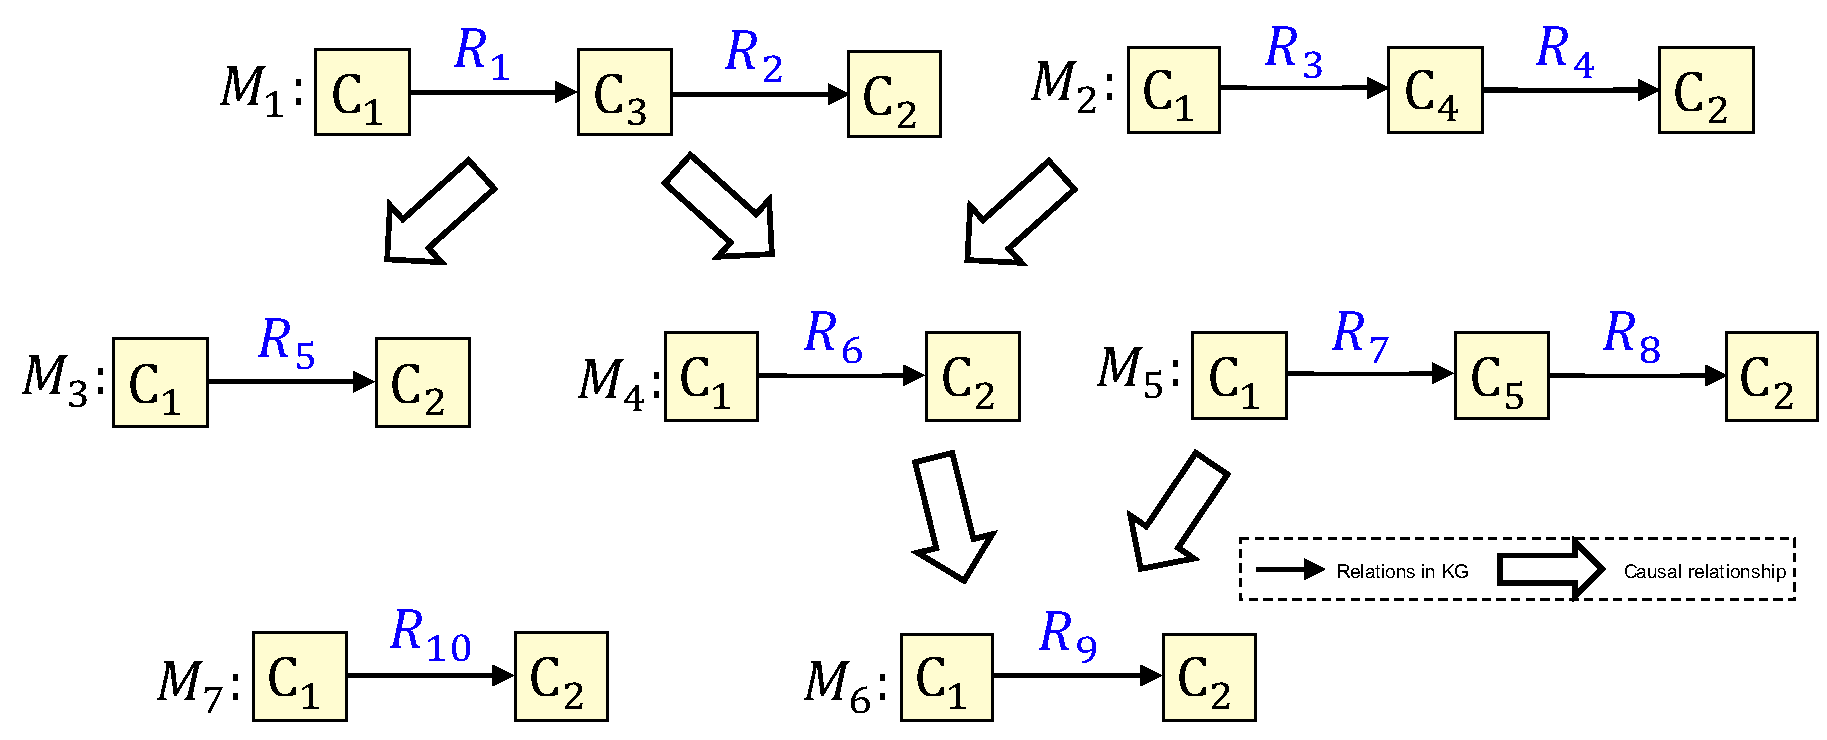
\includegraphics[width=8.5cm]{./figures/simulation.pdf}
% \caption{ The causal graph used to generate simulated knowledge graphs.}
% \label{fig:toy_example}
% \end{figure}

\begin{table}[t]
\centering
\caption{Dataset statistics of all the experiments.}
\label{tab:dataset_statistics}
% \vspace{-2pt}
\scalebox{1}{
\begin{tabular}{c|ccc}
\hline
   & \textbf{\#Triplets} & \textbf{\#Relations} & \textbf{\#Entities}  \\
\hline
\textbf{Simulation} & 6,095 & 5 & 1,590\\
\textbf{Douban Movie Rate} & 28,356 & 12 & 3,007 \\
\textbf{Hetionet} & 174,941 & 20 & 32,056 \\
\hline
\end{tabular}
}
\end{table}

\noindent
{\bf Simulation dataset.}
We generate simulated KGs based on a toy causal model specified in Fig.~\ref{fig:simulation}, which includes three concepts and five relations.
In particular, we design the causal mechanisms in KG via a probabilistic model.
The root nodes ($X_1$, $X_4$) in the causal graph are generated via Bernoulli distributions, whose probability mass function is $f_X(x)=p^x(1-p)^{1-x}$.
Moreover, the non-root nodes ($X_2$, $X_3$) are generated via the conditional probability distributions, which are Bernoulli distributions, given the parent node ($X_1$).
To maintain a stable causal mechanism, the parameters of conditional distributions are constant in training and testing, as shown in Table~\ref{tab:simulation_set}.
In the out-of-distribution paragraph, we will introduce the parameters of root nodes in training and testing.


\begin{figure}[h]
\centering
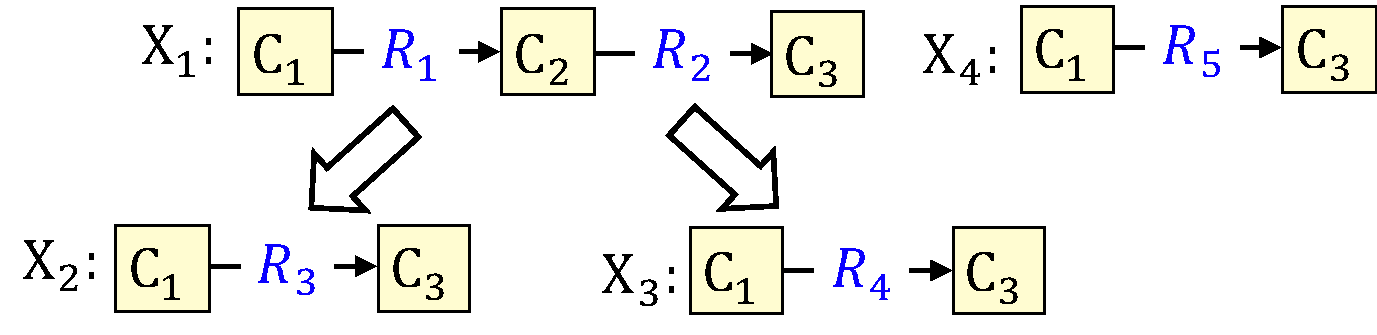
\includegraphics[width=7cm]{submissions/causal-meta-knowledge/figures/simulationv4.pdf}
\caption{The causal graph of relation paths, based on which the simulated KGs are generated .}
\label{fig:simulation}
% \vspace{-2pt}
\end{figure}

\begin{table}[h]
\caption{The parameters of conditional distributions.}
%\vspace{5pt}
\label{tab:simulation_set}
\centering
\scalebox{1}{
\begin{tabular}{c|cccc}
\hline
Conditions & $X_2|X_1=1$ & $X_2|X_1=0$ & $X_3|X_1=1$ & $X_3|X_1=0$ \\
\hline
Parameters & $p$=0.9 & $p$=0.1 & $p$=0.9 & $p$=0.1 \\
\hline
\end{tabular}}
% \vspace{-2pt}
\end{table}
% We generate simulated KGs based on a toy causal model specified in Fig.~\ref{fig:toy_example}, which includes five concepts and ten relations.
% More specifically, given $N$ entities for each concept, the facts containing the relations in the root nodes ($M_1$, $M_2$, $M_7$) of the causal graph are generated via Bernoulli distributions, whose probability mass function is $f(x)=p_r^x(1-p_r)^{1-x}$.
% For example, the entity pair $(e_1,e_3)$, where $e_1 \in \mathcal{E}_{C_1}$ and $e_3 \in \mathcal{E}_{C_3}$, the probability that the fact $<e_1,R_1,e_3> \in \mathcal{G}$ is $p_r$.
% % It means for any entity pair $(e_h,e_t)$, where $e_h \in \mathcal{E}_{C_h},\mathcal{E}_{C_t}$ and $R_i(C_h,C_t) \in \text{KG schema} \mathcal{S}$, the probability that the fact $R_i(e_h,e_t) \in \mathcal{T}$ is $p_r$.
% % we design the conditional  probabilistic distribution in SPRM based on which to sample the entity and facts in KG.
% And the facts in non-root nodes (e.g., $M_3$) are generated via the conditional probability distributions, which are Bernoulli distributions with parameter set $\mathbf{p}_{nr}$, given the facts information of parent node ($M_1$).
% For example, if there is a path instance of $M_1$ between $(e_1,e_3)$, then the probability of the existence of fact $<e_1,R_5,e_3>$ is $p_{M_1=1}$, otherwise is $p_{M_1=0}$.
% \yym{the value of all parameter of $p_nr$}

%


\noindent
{\bf Douban movie rating.}
Douban is a famous Chinese website for movie reviews, where users can rate and comment on any movie.
The rating range is from 1 to 5. A higher rating means that users like movies, while a lower rating means that users have negative feedback on movies.
We collect the real-world data from Douban\footnote{https://www.douban.com/} and construct a dataset (this dataset will be released), whose statistics are shown in Table~\ref{tab:dataset_statistics}.
Commonly, a movie with a score of 4 or 5 is identified as meeting the taste of users.
So we transform the original 5-level rating to a 2-level rating with a threshold of 4.
If the rating score is 4 or 5, the original relation \textit{Rate} is replaced by  \textit{HighRate}
We conduct the link prediction task on the relation \textit{HighRate}.
Because the raw data is too large and the relations between users and movies are very sparse, in this thesis, we first filter the 20 users who have made the most ratings and take the rating history of these users as the set of rating facts for our study.
The facts unrelated to the rating are also included in our experimental data.

\noindent
{\bf Hetionet}\cite{himmelstein2017systematic}
is a freely available knowledge database that integrates biomedical information from 29 prominent
bioinformatics resources.
Recently, Hetionet was successfully applied to drug repurposing tasks in terms of the link prediction task for relation \texttt{Treats}\cite{himmelstein2017systematic, ratajczak2022task}.

\textit{Why do we choose those two real datasets instead of other commonly used datasets, such as WN18, FB15k?}
In this paper, we focus on link prediction with the help of causal relationships between knowledge graph relations.
The core of causality lies in its asymmetry.
The commonly used KGs for link prediction algorithms contain many symmetrical relationships, e,g., \textit{hypernym} and \textit{hyponym} in WN18.
These symmetrical relationships may help with the link prediction task, but they go against the basic idea that causality is a one-way relationship.
We, therefore, chose datasets with specific application scenarios and rich causal semantics.

\subsubsection{\textbf{Metrics.}}
\textbf{For link prediction}, we employ the commonly used metrics mean reciprocal rank (MRR) and Hits@k~\cite{rossi2021knowledge,balazevic2019tucker,bordes2013translating}.
\begin{equation}
\label{eq:mrr}
\begin{aligned}
M R R=\frac{1}{|Q|} \sum_{q \in Q} \frac{1}{q}
\end{aligned}
\end{equation}

\begin{equation}
\label{eq:hitk}
\begin{aligned}
Hit@K=\frac{|\{q \in Q: q \leq K\}|}{|Q|}
\end{aligned}
\end{equation}
where $Q$ is the rank results, for each $q_i \in Q$ is the ranking of the desired results in the $i$-th query $(?,R_h,e_t)$.
In the case of ties in the calculation of $Q$, we use the mean rank to avoid misleading results\cite{rossi2021knowledge,ruffinelli2020you}.
% Common values for $K$ are 1, 3, 5, 10, we use $K=5$ in this paper.
Both MRR and His@k are the higher, the better.

\noindent
\textbf{The interpretability of causal rules} on the simulation dataset can be understood as the consistency between the mined causal rules and the actual causal structure.
Therefore, we evaluate baselines and our approach on the simulation dataset using precision, recall, and structural Hamming distance (SHD) as the evaluation metrics, which are commonly used evaluation metrics in causal structure discovery studies~\cite{zheng2018dags,zheng2020learning}.
% Since the performance of causal rule discovery is the foundation of our link prediction method.

\begin{equation}
\label{eq:precision}
\begin{aligned}
Precision=\frac{\# TFR}{\#FR};Recall=\frac{\# TFR}{\#ATR}
\end{aligned}
\end{equation}
Where $\#TFR$ is the number of right causal relationships discovered by an algorithm, $\#FR$ is the number of causal relationships discovered by an algorithm, and $\#ATR$ is the number of all causal relationships.
Both precision and recall are the higher, the better.
SHD calculates the difference between the learned graph and the ground truth graph by the number of edge insertions, deletions, or flips required to transform one graph into another.
The lower the SHD, the better.

\subsubsection{\textbf{Out-of-Distribution Link Prediction}}
Traditional machine learning methods are designed based on the assumption of independent and identically distributed (I.I.D) data.
This assumption means the training and test data come from the same distribution. However, the distribution of test data may alter due to changes in the test environment; such tasks are referred to as OoD tasks.
Traditional algorithms perform poorly on generalization problems due to the violation of I.I.D assumption.
Causality is seen as a stable inference mechanism in many research works on generalization problems.
So, in this work, we provide an out-of-distribution generalization task for the knowledge link prediction task for the first time.
On the one hand, the effect of causal metaknowledge on this task can be measured, and on the other, the performance of existing algorithms can be looked at.
We also evaluate the performance of the algorithms on I.I.D link prediction tasks.

In this paper, we design two OoD experimental scenarios.

\noindent
(1) \textit{Simulation dataset}:
We evaluate the link prediction performance under I.I.D and OoD settings, where the triples of root node $X_1$ are generated in testing under the same and different parameters with training.
In the training and I.I.D testing datasets, $p_{X_1}=0.5$.
In the OoD testing datasets, $p_{X_1} \in \{0.2,0.9\}$.
For $X_4$, $p_{X_4}$ maintains $0.9$ in training and testing.
The facts of the KGs are split into three parts:\textit{train}, \textit{test info}, and \textit{test}.
The facts in \textit{train} are used to learn the rule.
The effectiveness of the learned rule is assessed via the link prediction task on $R_3$.
The \textit{test info} part includes facts of new entities (did not appear in \textit{train}) on $R_1, R_2, R_4, R_5$, and \textit{test} part includes the queried facts on $R_3$.

\noindent
(2)\textit{Real datasets}:
It is impossible to explicitly change the data distribution since real data distribution is inaccessible for real datasets.
Recent research\cite{tang2020investigating,wu2021self} has suggested that graph models are biased towards nodes with larger degrees, which causes the bad performance of low-degree nodes in the test.
Therefore we construct the OoD datasets based on degree shift.
Specifically, given a query task $(?,R_h,e_t)$, we calculate the \textit{median} of degree\footnote{In this paper, we use the term "degree" to stand for the sum of in and out degrees} of known entities $e_t$ belonging to the triples $(e_h,R_h,e_t)$ in the training.
Then we bin the test queries by the degrees of the known entities $e_t$.
The degree range in each bucket is decided based on the sample size balance.
The test queries in the bucket, which the training median falls in, can be treated as the I.I.D test samples.
Others are the OoD samples.
The I.I.D bucket is labeled with $*$ in Table~\ref{tab:douban-mrr} and Table~\ref{tab:hetionet-mrr}.





\subsection{Performance of Link prediction task in Out-of-Distrition Settings}

\noindent
\textbf{Results on simulations.}
For the simulation dataset, we construct a OoD setting named as covariance shift, by changing the probability distribution of the root nodes in the test phase.
Table~\ref{tab:simulation_result} presents the methods in performance and demonstrates the effectiveness of the proposed \dname.
In particular, \dname~outperforms the baseline models under all metrics except the Hits@10 under I.I.D setting. This shows our method can give a stable and high-quality result, especially in the OOD setting.
Besides, compared with the baselines, the proposed \dname~ perform significantly better at the Hits@1 metric (at least 25\% absolute improvements that the second place under all settings), which suggests the our method are more suitable for scenarios with strict performance requirements, and this feature may achieved by the removal of association-based rules.

\begin{table}[h]
\caption{The results of link prediction on simulation datasets.}
\centering
\label{tab:simulation_result}
\scalebox{1.2}{
\begin{tabular}{c|c|l|cccc}
\hline
 \multirow{2}{*}{\textbf{Settings}}& \multirow{2}{*}{$\mathbf{p_{X_1}}$} & \multirow{2}{*}{\textbf{Method}} & \multirow{2}{*}{\textbf{MRR}} & \multicolumn{3}{c}{\textbf{Hits}} \\ \cline{5-7}
& & & &\textbf{@10} & \textbf{@3} & \textbf{@1} \\ \hline
\multirow{4}{*}{I.I.D} & \multirow{4}{*}{0.5}
& AMIE+ & 0.87 & \textbf{98.99} & 94.95 & 78.79\\
&  & AnyBURL & 0.87 &\textbf{98.99}&94.95 &78.79\\
&  & Neural-LP &  0.80 & \textbf{98.99} & 92.42& 66.16\\
& & RNNLogic & 0.87 & \textbf{98.99} & 94.95 & 78.79\\
&& \dname & \textbf{0.94} & 98.48&\textbf{97.98} &\textbf{90.91}\\

 \hline
\multirow{4}{*}{OOD} & \multirow{4}{*}{0.2}
& AMIE+ & 0.875 & 96.91 & 93.81 & 81.44 \\
&  & AnyBURL &  0.875 & 96.91&93.81 & 81.44\\
& & Neural-LP & 0.68 & 98.97 & 79.38 & 50.51\\
& & RNNLogic & 0.875 & 96.91 & 93.81 & 81.44 \\
&& \dname & \textbf{0.99} & \textbf{100}&\textbf{100} &\textbf{99.97}\\
 \hline
 \multirow{4}{*}{OOD} & \multirow{4}{*}{0.9}
& AMIE+ & 0.91 & \textbf{100} & 96.34 & 85.67 \\
&  & AnyBURL &  0.91 &\textbf{100} & 96.34 & 85.67\\
& & Neural-LP & 0.88 & \textbf{100} & 96.95 & 79.57\\
& & RNNLogic & 0.91 & \textbf{100} & 96.34 & 85.67 \\
&& \dname & \textbf{0.99} &  \textbf{100}& \textbf{99.70} & \textbf{99.09}\\
 \hline
\end{tabular}
}
\end{table}

% Also we considered the effect of different score functions on the link prediction performance.
% The results are shown in Tab.~\ref{tab:simulation_result}, and  can find that our method also works well for the simulated data, especially under OoD settings. Specifically, our model gets the best MRR and Hit@1 results, while AMIE+ and AnyBURL are the best methods for Hit@5 and Hit@10 for I.I.D setting. This may be because they tend to discover more rules, while our method aims to identity the causality more accurately, so fewer links are predicted.
% For OoD data, the proposed method surpasses all baseline models on all metrics, which fully support our motivation: building a link prediction algorithm with strong generalization ability.

% Overall, our method performs best for all three datasets. Also note although some baselines get the best results under some specific settings, they can not maintain a good performance for other settings or metrics. For example, TuckER gets the best MRR under 0-5 degree range, while performs worst with 30-60 degree range on Douban movie rating dataset. By contrast, the proposed CMLP can achieve best or competitive results for all settings.

% \yym{Prior systems for generating conjectures have either contributed genuinely useful research conjectures9 via methods that do not easily generalize to other mathematical areas10, or have dem- onstrated novel, general methods for finding conjectures11 that have not yet yielded mathematically valuable results.}


% \begin{table}[h]
% \caption{The results of link prediction on simulation datasets.}
% \centering
% \label{tab:simulation_result}
% \scalebox{1}{
% \begin{tabular}{c|c|l|cccc}
% \hline
%  \multirow{2}{*}{\textbf{Settings}}& \multirow{2}{*}{$\mathbf{p_{r}}$} & \multirow{2}{*}{\textbf{Method}} & \multirow{2}{*}{\textbf{MRR}} & \multicolumn{3}{c}{\textbf{Hits}} \\ \cline{5-7}
% & & & &\textbf{@1} & \textbf{@5} & \textbf{@10} \\ \hline
% \multirow{5}{*}{I.I.D} & \multirow{5}{*}{0.3}
% & AMIE+ & 0.734 & 0.589 & \textbf{0.948} & \textbf{1}\\
% &  & AnyBURL & 0.733 & 0.589 & \textbf{0.948} & \textbf{1}\\
% &  & Neural-LP &  0.58 & 0.41 & 0.743 & 0.769\\
% &  & RNNLogic &  0.603 & 0.461 & 0.666 & 0.666\\
% & & \dname & \textbf{0.785} & \textbf{0.692} & 0.897 & 0.897 \\

% %  \hline
% % \multirow{5}{*}{OOD} & \multirow{5}{*}{0.1}
% % & AMIE+ & 0.73 & 0.538 & \textbf{0.846} & \textbf{0.846} \\
% % &  & AnyBURL &  \textbf{0.782} & \textbf{0.615} & \textbf{0.846} & \textbf{0.846} \\
% % & & Neural-LP & 0.673 & 0.461 & 0.769 & 0.769\\
% % & & RNNLogic & 0.611 & 0.307 & 0.538 & 0.538\\
% % && \dname & 0.692 & 0.538 & 0.692 & 0.692\\
%  \hline
%  \multirow{5}{*}{OOD} & \multirow{5}{*}{0.8}
% & AMIE+ & 0.891 & 0.843 & \textbf{0.98} & \textbf{1} \\
% &  & AnyBURL &  0.893 & 0.843 & \textbf{0.98} & \textbf{1}\\
% & & Neural-LP & 0.885 & 0.843 & 0.941 & 0.98\\
% & & RNNLogic & 0.853 & 0.803 & 0.882 & 0.882\\
% && \dname & \textbf{0.909} &  \textbf{0.862} & \textbf{0.98} & \textbf{1}\\
%  \hline
% \end{tabular}
% }
% \end{table}
\noindent
\textbf{Results for Douban movie rating.}
Since we filtered the users of the Douban data, and the discrepancies of the degrees of experimental user nodes are close to each other.
Therefore, in this experiment, to construct the OoD scenario, we adopt the head prediction (? , HighRate, Movie), predicting the set of users who gave high ratings to movies.
Further, we bucketed the movie nodes in the test data according to their degree in the training data to observe the performance of the algorithm under different node prevalence.
The MRR and Hits@5 results shown in
Tab.~\ref{tab:douban-mrr} shows that the proposed CMLP get the best performance in the all OoD settings.
Especially, at least 25.8\% and 29.3 \% relative improvements that the second place on the MRR and Hits@5, respectively.
In the I.I.D setting, ~\dname~gets the second place on both MRR and Hits@5, lower than the representation-based method TuckER.
These results illustrate that for movie
rating datasets, the rules learned by our method can capture more general user preferences and give relatively accurate rating predictions for movies that are in different popularity.





% sum query head
\begin{table}[]
\centering
\caption{MRR (left) and Hits@5 (right) for Douban movie rating. The * marks columns that contain the I.I.D results. Other columns contain OoD results.}
\label{tab:douban-mrr}
\scalebox{1.2}{
\begin{tabular}{c|ccccc}
\hline
\multirow{2}{*}{\textbf{Methods}} & \multicolumn{4}{c}{\textbf{Degree Range}} \\ \cline{2-5}
          & \textbf{0-21*}   & \textbf{21-31}   & \textbf{31-39} & \textbf{39-60} \\ \hline
AMIE+     & 0.120 & 0.205 & 0.261 & 0.395 \\
AnyBURL   & 0.125 & 0.182  & 0.231 & 0.373 \\
Neural-LP & 0.078 & 0.097  & 0.126 & 0.217 \\
RNNLogic  & 0.072 & 0.086  & 0.097 & 0.161 \\
TuckER    & \textbf{0.287} & 0.186  &  0.186 & 0.149 \\
\dname      & 0.251 & \textbf{0.343}  & \textbf{0.392} & \textbf{0.497}\\ \hline
\end{tabular}
\quad
\begin{tabular}{c|ccccc}
\hline
\multirow{2}{*}{\textbf{Methods}} & \multicolumn{4}{c}{\textbf{Degree Range}} \\ \cline{2-5}
         & \textbf{0-21*}    & \textbf{21-31}   & \textbf{31-39} & \textbf{39-60}  \\ \hline
AMIE+        & 13.7 &30.7  & 39.4  & 68.3  \\
AnyBURL      & 15.1  & 26.0  & 33.2 & 64.6  \\
Neural-LP    & 0.1      & 0.6     & 3.4     & 60.0 \\
RNNLogic     & 1.6    & 4.7  & 7.2 & 13.5  \\
TuckER     & \textbf{50.3}   & 31.9   & 28.2  &  21.5 \\
\dname     & 40.9  & \textbf{60.0}  & \textbf{68.1} & \textbf{88.3}  \\ \hline
\end{tabular}}
\end{table}


% \begin{table}[]

% \caption{Hits@5 for Douban movie rating. The * marks columns that contain the I.I.D results. Other columns contain OoD results.}
% \label{tab:douban-hits1}
% \begin{tabular}{c|ccccc}
% \hline
% \multirow{2}{*}{\textbf{Methods}} & \multicolumn{4}{c}{\textbf{Degree Range}} \\ \cline{2-5}
%          & \textbf{0-21*}    & \textbf{21-31}   & \textbf{31-39} & \textbf{39-60}  \\ \hline
% AMIE+        & 13.7 &30.7  & 39.4  & 68.3  \\
% AnyBURL      & 15.1  & 26.0  & 33.2 & 64.6  \\
% Neural-LP    & 0.1      & 0.6     & 3.4     & 60.0 \\
% RNNLogic     & 1.6    & 4.7  & 7.2 & 13.5  \\
% TuckER     & \textbf{50.3}   & 31.9   & 28.2  &  21.5 \\
% \dname     & 40.9  & \textbf{60.0}  & \textbf{68.1} & \textbf{88.3}  \\ \hline
% \end{tabular}
% \end{table}

\noindent
\textbf{Results for drug repurposing on Hetionet.}
Consistent with the traditional setup of drug redirection, on Hetionet, we also use head predition (?, Treat, Disease), which is giving a Disease to predict new drugs. We also observe the performance of the algorithm under this task by bucketing for Disease node degrees.
Tab.~\ref{tab:hetionet-mrr} reports the MRR and Hits@5 on this dataset, and we can find that: our CMLP performs significantly better than other baselines on low-degree diseases (0-17), while AMIE+ and AnyBURL get better results on low-degree diseases (17-100).
These results indicate that our method can give more accurate drug discovery results for diseases with relatively low information.
And for diseases with richer information, the correlation-based inference rules give more accurate drug prediction.


\begin{table}[]
\centering
\caption{MRR(left) and Hits@5(right) for drug repurposing on Hetionet. The * marks columns that contain the I.I.D results. Other columns contain OoD results.}
\label{tab:hetionet-mrr}
\scalebox{1.2}{
\begin{tabular}{c|ccccc}
\hline
\multirow{2}{*}{\textbf{Methods}} & \multicolumn{4}{c}{\textbf{Degree Range}} \\ \cline{2-5}
    & \textbf{0-8*}    & \textbf{8-17}   & \textbf{17-31}  & \textbf{31-100} \\ \hline
AMIE+   & 0.103  & 0.085  & \textbf{0.132}  & 0.065 \\
AnyBURL  & 0.116   & 0.189  & 0.090  & \textbf{0.188} \\
Neural-LP & 0.027  & 0.014  & 0.009  & 0.009 \\
RNNLogic & 0.07  & 0.021  & 0.029  & 0.012 \\
TuckER  &  0.044  & 0.022    & 0.083   &  0.015 \\
\dname  & \textbf{0.248}  & \textbf{0.208}  & 0.095 & 0.093 \\ \hline
\end{tabular}
\quad
\begin{tabular}{c|cccc}
\hline
\multirow{2}{*}{\textbf{Methods}} & \multicolumn{4}{c}{\textbf{Degree Range}} \\ \cline{2-5}
  & \textbf{0-8*}    & \textbf{8-17}   & \textbf{17-31}  & \textbf{31-100} \\
  \hline
AMIE+      & 13.2  & 11.3  & \textbf{22.5} & 13.2  \\
AnyBURL     & 15.8  & \textbf{25.0}  & 9.6  & \textbf{23.7}   \\
Neural-LP   & 5.3      & 0     & 0      & 0      \\
RNNLogic  & 7.9  & 0  & 3.2      & 0      \\
TuckER    &  3.1   & 5.9  &  10.7  &  3.2   \\
\dname     & \textbf{26.31}  & \textbf{25.0} & 16.1 & 13.1  \\ \hline
\end{tabular}}
\end{table}

% \begin{table}[]

% \caption{MRR for drug repurposing on Hetionet. The * marks the range in which the mean of the training data falls.}
% \label{tab:hetionet-mrr}
% \begin{tabular}{c|ccccc}
% \hline
% \multirow{2}{*}{\textbf{Methods}} & \multicolumn{3}{c}{\textbf{Degree Range}} \\ \cline{2-4}
%     & \textbf{0-5}    & \textbf{5-15*}   & \textbf{15-30}   \\ \hline
% AMIE+   & 0.277  & 0.103  & 0.126   \\
% AnyBURL  & 0.28   & 0.177  & 0.134  \\
% Neural-LP & 0.036  & 0.016  & 0.011  \\
% RNNLogic & 0.149  & 0.038  & 0.023   \\
% TuckER  &  0.085  & 0.021    & 0.078    \\
% \dname  & \textbf{0.329}  & \textbf{0.327}  & \textbf{0.261} \\ \hline
% \end{tabular}
% \end{table}

% \begin{table}[]

% \caption{Hits@5 for drug repurposing on Hetionet. The * marks columns that contain the I.I.D results. Other columns contain OoD results.}
% \label{tab:hetionet-hits1}
% \begin{tabular}{c|cccc}
% \hline
% \multirow{2}{*}{\textbf{Methods}} & \multicolumn{4}{c}{\textbf{Degree Range}} \\ \cline{2-5}
%   & \textbf{0-8*}    & \textbf{8-17}   & \textbf{17-31}  & \textbf{31-100} \\
%   \hline
% AMIE+      & 13.2  & 11.3  & \textbf{22.5} & 13.2  \\
% AnyBURL     & 15.8  & \textbf{25.0}  & 9.6  & \textbf{23.7}   \\
% Neural-LP   & 5.3      & 0     & 0      & 0      \\
% RNNLogic  & 7.9  & 0  & 3.2      & 0      \\
% TuckER    &  3.1   & 5.9  &  10.7  &  3.2   \\
% \dname     & \textbf{26.31}  & \textbf{25.0} & 16.1 & 13.1  \\ \hline
% \end{tabular}
% \end{table}

% \begin{table}[]

% \caption{Hits@1 for drug repurposing on Hetionet. The * marks the range in which the mean of the training data falls.}
% \label{tab:hetionet-hits1}
% \begin{tabular}{c|cccc}
% \hline
% \multirow{2}{*}{\textbf{Methods}} & \multicolumn{3}{c}{\textbf{Degree Range}} \\ \cline{2-4}
%   & \textbf{0-5}    & \textbf{5-15*}  & \textbf{15-30}   \\ \hline
% AMIE+      & 0.111  & 0.02  & 0.027   \\
% AnyBURL     & 0.111  & 0.06  & 0.027     \\
% Neural-LP   & 0      & 0     & 0            \\
% RNNLogic  & 0.055  & 0.02  & 0          \\
% TuckER    &  0.071   & 0  &  0.064    \\
% \dname     & \textbf{0.166}  & \textbf{0.14}  & \textbf{0.138}   \\ \hline
% \end{tabular}
% \end{table}

\noindent


% \begin{table}[h]
% \caption{The results of link prediction on simulation datasets. The adopted score function is AVG.}
% \centering
% \label{tab:simulation_result2}
% \scalebox{1}{
% \begin{tabular}{c|c|l|cccc}
% \hline
%  \multirow{2}{*}{\textbf{Settings}}& \multirow{2}{*}{$\mathbf{p_{r}}$} & \multirow{2}{*}{\textbf{Method}} & \multirow{2}{*}{\textbf{MRR}} & \multicolumn{3}{c}{\textbf{Hits}} \\ \cline{5-7}
% & & & &\textbf{@1} & \textbf{@5} & \textbf{@10} \\ \hline
% \multirow{5}{*}{I.I.D} & \multirow{5}{*}{0.3}
% & AMIE+ & 0.829 & 0.717 & \textbf{0.974} & \textbf{1}\\
% &  & AnyBURL & 0.829 & 0.717 & \textbf{0.974} & \textbf{1}\\
% &  & Neural-LP &  0.619 & 0.435 & 0.769 & 0.769\\
% &  & RNNLogic &  0.684 & 0.589 & 0.666 & 0.666\\
% & & \dname & \textbf{0.868} & \textbf{0.82} & 0.897 & 0.897 \\

% %  \hline
% % \multirow{5}{*}{OOD} & \multirow{5}{*}{0.1}
% % & AMIE+ & \textbf{0.807} & \textbf{0.692} & \textbf{0.846} & \textbf{0.846} \\
% % &  & AnyBURL &  \textbf{0.807} & \textbf{0.692} & \textbf{0.846} & \textbf{0.846} \\
% % & & Neural-LP & 0.711 & 0.538 & 0.769 & 0.769\\
% % & & RNNLogic & 0.807 & 0.461 & 0.538 & 0.538\\
% % && \dname & 0.769 & \textbf{0.692} & 0.692 & 0.692\\
%  \hline
%  \multirow{5}{*}{OOD} & \multirow{5}{*}{0.8}
% & AMIE+ & 0.887 & 0.823 & \textbf{1} & \textbf{1} \\
% &  & AnyBURL &  0.887 & 0.823 & \textbf{1} & \textbf{1}\\
% & & Neural-LP & 0.85 & 0.784 & 0.98 & 0.98\\
% & & RNNLogic & 0.898 & 0.882 & 0.882 & 0.882\\
% && \dname & \textbf{1} &  \textbf{1} & \textbf{1} & \textbf{1}\\
%  \hline
% \end{tabular}
% }
% \end{table}

\subsection{Quality and Interpretability  of Causal Rules.}

As stated in Sec.~\ref{section:introduction}, the mined rules play a key role in our algorithm, and an important advantage of these rules is that they are well interpretable.
In this section, we will evaluate the quality and interpretability of rules mined by \dname~.


% % In this section, we explore the performance of~\dname~on causal rule mining.
% With the aid of simulation data, we can quantitatively evaluate the ability of different rule-based algorithms for the discovery of causal graph structure in Fig.~\ref{fig:toy_example}.
% In particular we introduce a classical algorithm PC\cite{abellan2006some}for causal discovery of propositional data as an additional baseline.
% The results are shown in Fig.\ref{fig:sim-graph}, and we can get the following observations:
% (i) The proposed show a good overall performs on all metrics, {\it i.e.} precision, recall, and SHD.
% (ii) The deep learning-based approaches, {\it i.e.} Neural-LP and RNNLogic, are hard to obtain good performances on these metrics. The low recall of them suggests that they have difficulty in mining interpretable rules.



% \begin{table*}[h]
% \caption{All rules whose head are $R_5$, $R_6$ and $R_9$, obtained by each algorithm learned on simulated dataset. The rules with red text are the wrong results which are not consistent with the generation process.\lsx{Why so few for CMLP}
% % The orange text denotes the weight of each rule with the form max-normalization(original weight)
% }.
% \label{tab:simulation_rule}
% \centering
% \scalebox{0.8}{
% \begin{tabular}{c|l|l|l}

% \hline
% \textbf{Method} & \textbf{Rules of $R_5$} & \textbf{Rules of $R_6$} & \textbf{Rules of $R_9$} \\

% \hline
% \multirow{3}{*}{\dname} &
% $R_5(C_1,C_2) \gets R_1(C_1,C_3), R_2(C_3,C_2)$ &
% $R_6(C_1,C_2) \gets R_3(C_1,C_4), R_4(C_4,C_2)$  &
% $R_9(C_1,C_2) \gets R_6(C_1,C_2)$ \\
% & & \color{red}{$R_6(C_1,C_2) \gets R_9(C_1,C_2)$} &
% $R_9(C_1,C_2) \gets R_7(C_1,C_5), R_8(C_5,C_2)$ \\
% & & $R_6(C_1,C_2) \gets R_1(C_1,C_3), R_2(C_3,C_2)$ &  \\
% \hline
% \multirow{6}{*}{AMIE+} &
% $R_5(C_1,C_2) \gets R_1(C_1,C_3), R_2(C_3,C_2)$ &
% $R_6(C_1,C_2) \gets R_3(C_1,C_4), R_4(C_4,C_2)$ &
% $R_9(C_1,C_2) \gets R_7(C_1,C_5), R_8(C_5,C_2)$ \\
% & \color{red}{$R_5(C_1,C_2) \gets R_6(C_1,C_2)$} &
% \color{red}{$R_6(C_1,C_2) \gets R_9(C_1,C_2)$} &
% $R_9(C_1,C_2) \gets R_6(C_1,C_2)$ \\
% & \color{red}{$R_5(C_1,C_2) \gets R_9(C_1,C_2)$} &
% $R_6(C_1,C_2) \gets R_1(C_1,C_3), R_2(C_3,C_2)$ &
% \color{red}{$R_9(C_1,C_2) \gets R_3(C_1,C_4), R_4(C_4,C_2)$} \\
% & \color{red}{$R_5(C_1,C_2) \gets R_7(C_1,C_5), R_8(C_5,C_2)$}
% & \color{red}{$R_6(C_1,C_2) \gets R_5(C_1,C_2)$} &
% \color{red}{$R_9(C_1,C_2) \gets R_{10}(C_1,C_2)$} \\
% & \color{red}{$R_5(C_1,C_2) \gets R_3(C_1,C_4), R_4(C_4,C_2)$} &
% \color{red}{$R_6(C_1,C_2) \gets R_{10}(C_1,C_2)$} &
% \color{red}{$R_9(C_1,C_2) \gets R_1(C_1,C_3), R_2(C_3,C_2)$} \\
% & \color{red}{$R_5(C_1,C_2) \gets R_{10}(C_1,C_2)$} &
% \color{red}{$R_6(C_1,C_2) \gets R_7(C_1,C_5), R_8(C_5,C_2)$} &
% \color{red}{$R_9(C_1,C_2) \gets R_5(C_1,C_2)$} \\

% \hline
% % $R_3(C_1,C_3) \gets R_1(C_1,C_2), R_2(C_2,C_3)$
% \multirow{6}{*}{AnyBURL} &
% $R_5(C_1,C_2) \gets R_1(C_1,C_3), R_2(C_3,C_2)$ &
% $R_6(C_1,C_2) \gets R_3(C_1,C_4), R_4(C_4,C_2)$ &
% $R_9(C_1,C_2) \gets R_7(C_1,C_5), R_8(C_5,C_2)$ \\ &
% $ \color{red}{R_5(C_1,C_2) \gets R_7(C_1,C_5), R_8(C_5,C_2)}$ &
% $ \color{red}{R_6(C_1,C_2) \gets R_9(C_1,C_2)}$ &
% $ R_9(C_1,C_2) \gets R_6(C_1,C_2)$ \\ &
% $ \color{red}{R_5(C_1,C_2) \gets R_{10}(C_1,C_2)}$ &
% $R_6(C_1,C_2) \gets R_1(C_1,C_3), R_2(C_3,C_2)$ &
% $ \color{red}{R_9(C_1,C_2) \gets R_{10}(C_1,C_2)}$ \\ &
% $ \color{red}{R_5(C_1,C_2) \gets R_6(C_1,C_2)}$ &
% $ \color{red}{R_6(C_1,C_2) \gets R_5(C_1,C_2)}$ &
% $ \color{red}{R_9(C_1,C_2) \gets R_3(C_1,C_4), R_4(C_4,C_2)}$ \\ &
% $ \color{red}{R_5(C_1,C_2) \gets R_9(C_1,C_2)}$ &
% $ \color{red}{R_6(C_1,C_2) \gets R_{10}(C_1,C_2)}$ &
% $ \color{red}{R_9(C_1,C_2) \gets R_1(C_1,C_3), R_2(C_3,C_2)}$ \\ &
% $ \color{red}{R_5(C_1,C_2) \gets R_3(C_1,C_4), R_4(C_4,C_2)}$ &
% $ \color{red}{R_6(C_1,C_2) \gets R_7(C_1,C_5), R_8(C_5,C_2)}$ &
% $ \color{red}{R_9(C_1,C_2) \gets R_5(C_1,C_2)}$ \\
% \hline

% \multirow{4}{*}{Neural-LP} &
% $ \color{red}{R_5(C_1,C_2) \gets R_6(C_1,C_2)}$ &
% $ \color{red}{R_6(C_1,C_2) \gets R_9(C_1,C_2)}$ &
% $ \color{red}{R_9(C_1,C_2) \gets R_{10}(C_1,C_2)}$ \\ &
% $ \color{red}{R_5(C_1,C_2) \gets R_9(C_1,C_2)}$ &
% $ \color{red}{R_6(C_1,C_2) \gets R_{10}(C_1,C_2)}$ &
% $ \color{red}{R_9(C_1,C_2) \gets R_5(C_1,C_2)}$ \\ &
% $ \color{red}{R_5(C_1,C_2) \gets R_{10}(C_1,C_2)}$ &
% $ \color{red}{R_6(C_1,C_2) \gets R_5(C_1,C_2)}$ &
% $R_9(C_1,C_2) \gets R_6(C_1,C_4)$ \\ &&&
% $ \color{red}{R_9(C_1,C_2) \gets R_9(C_1,C_2)}$ \\
% \hline

% \multirow{2}{*}{RNNLogic} &
% $ \color{red}{R_5(C_1,C_2) \gets R_6(C_1,C_2)}$ &
% $ \color{red}{R_6(C_1,C_2) \gets R_5(C_1,C_2)}$ &
% $R_9(C_1,C_2) \gets R_6(C_1,C_2)$ \\ &&
% $ \color{red}{R_6(C_1,C_2) \gets R_9(C_1,C_2)}$ &
% $ \color{red}{R_9(C_1,C_2) \gets R_{10}(C_1,C_2)}$ \\
% \hline
% % \tabucline[1pt]{-}
% \end{tabular}}
% \end{table*}


% \begin{figure*}[t]
%     \centering
%     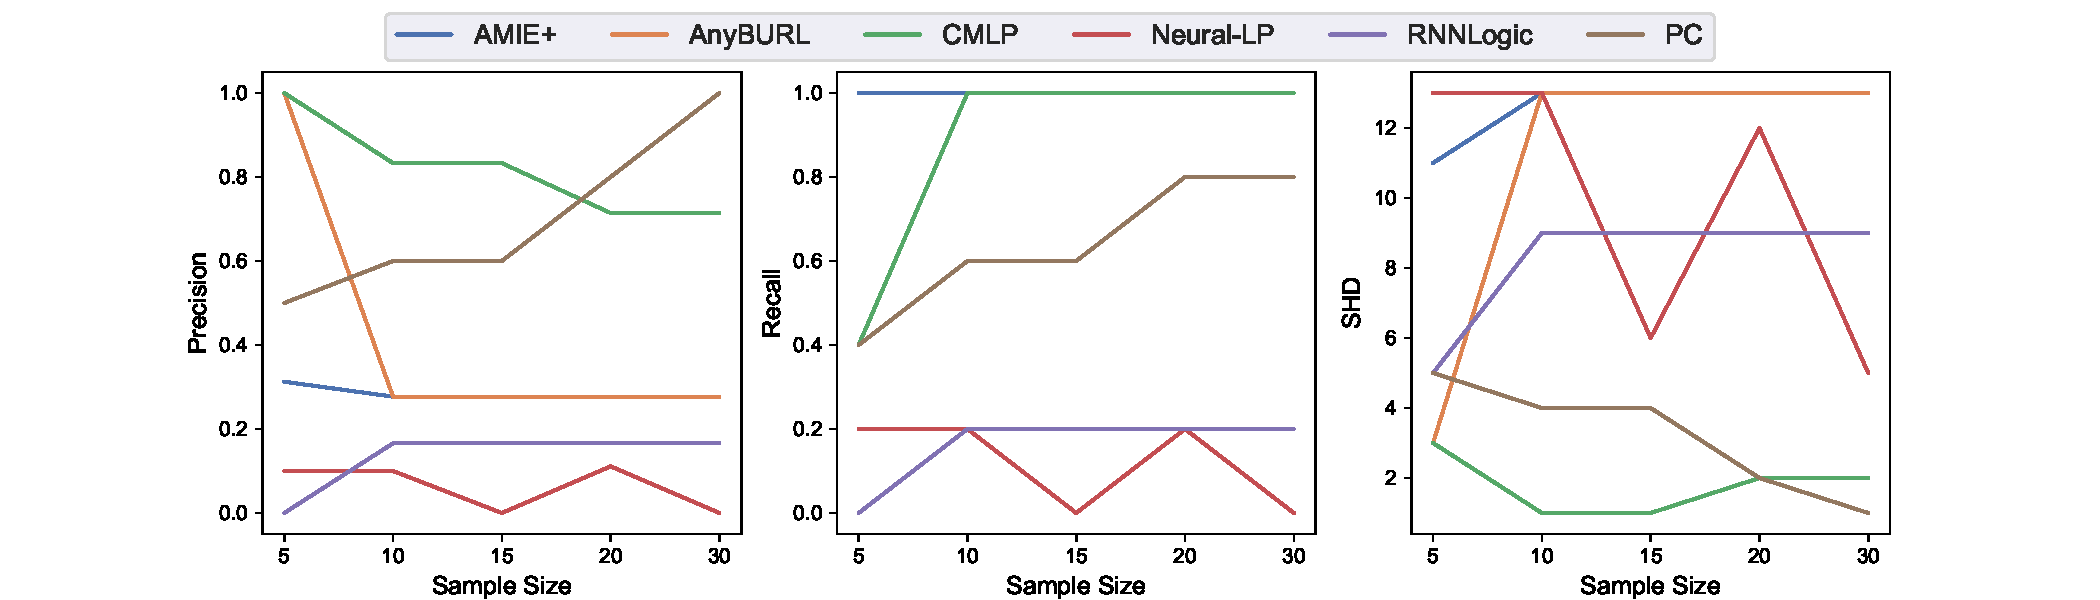
\includegraphics[trim=3cm 0cm 3cm 0cm, width=\linewidth, height=5cm]{figures/allin.pdf}
%     \caption{Precision, recall and SHD results on simulation datasets with differnet sample size. }
%     \label{fig:sim-graph}
% \end{figure*}
\noindent
\textbf{Quality of causal rules from simulations.}
The ground-truth causal graph of KGSs shown in Fig~\ref{fig:simulation}, and
Table~\ref{tab:simulation_rule_quality} shows the accuracy of estimated rules of different methods.
In particular, \dname~ accurately discovers two causal rules in Fig~\ref{fig:simulation} without any redundant rules.
In contrast, correlation-based methods report some non-causal rules.


\begin{table}[t]
\caption{Experimental results on simulation data with $p_{X_1}=0.5$, based on the metrics (precision, recall and SHD), which are commonly used to evaluate the estimated causal graph.}
%\vspace{5pt}
\label{tab:simulation_rule_quality}
\centering
\scalebox{1.2}{
\begin{tabular}{c|c|c|c}
\hline
\textbf{Method} & \textbf{Precision} $\uparrow$ & \textbf{Recall} $\uparrow$ & \textbf{SHD} $\downarrow$ \\
\hline
Neural-LP & 0 & 0& 10 \\
AMIE+ & 0.22 & \textbf{1.0}& 7 \\
RNNLogic & 0.22 & \textbf{1.0}& 7 \\
AnyBURL & 0.25 & \textbf{1.0}& 6 \\
\dname & \textbf{1.0} & \textbf{1.0} & \textbf{0} \\
\hline
\end{tabular}}
\vspace{-4pt}
\end{table}

\begin{table*}[h]
\caption{All rules whose head are $R_3$ and $R_5$, obtained by each algorithm learned on simulated dataset. The strikethroughs indicate the wrong results (there is no entities satisfying the rule).
The rules consistent with the generation process are in bold.
The orange text denotes the weight of each rule with the form max-normalization(original weight)}.

\label{tab:simulation_rule}
\centering
{\tiny
\scalebox{0.75}{
\begin{tabu}{c|l|l|l}
\tabucline[1pt]{-}
\textbf{Method} & \textbf{Rules of $R_3$ with $\mathbf{p_{X_1}=0.5}$} & \textbf{Rules of $R_3$ with $\mathbf{p_{X_1}=0.9}$} & \textbf{Rules of $R_5$}\\
\tabucline[1pt]{-}

\multirow{3}{*}{AMIE+} & \textcolor{orange}{1.00 (0.908)}   $\mathbf{R_3(C_1,C_3) \gets R_1(C_1,C_2), R_2(C_2,C_3)}$  & \textcolor{orange}{1.00 (0.900)}   $\mathbf{R_3(C_1,C_3) \gets R_1(C_1,C_2), R_2(C_2,C_3)}$ & \textcolor{orange}{1.00 (0.898)}   $R_5(C_1,C_3) \gets R_1(C_1,C_2), R_2(C_2,C_3)$\\

& \textcolor{orange}{0.91 (0.829)}   $R_3(C_1,C_3) \gets R_4(C_1,C_3)$ & \textcolor{orange}{0.99 (0.890)}   $R_3(C_1,C_3) \gets R_4(C_1,C_3)$ & \textcolor{orange}{0.99 (0.895)}   $R_5(C_1,C_3) \gets R_3(C_1,C_3)$ \\
&  \textcolor{orange}{0.55 (0.500)}   $R_3(C_1,C_3) \gets R_5(C_1,C_3)$  & \textcolor{orange}{0.91 (0.820)}   $R_3(C_1,C_3) \gets R_5(C_1,C_3)$ & \textcolor{orange}{0.99 (0.894)}   $R_5(C_1,C_3) \gets R_4(C_1,C_3)$\\
\hline
\multirow{3}{*}{AnyBURL}& \textcolor{orange}{1.00 (0.896)} $\mathbf{R_3(C_1,C_3) \gets R_1(C_1,C_2), R_2(C_2,C_3)}$ & \textcolor{orange}{1.00 (0.898)} $R_3(C_1,C_3) \gets R_4(C_1,C_3)$ & \textcolor{orange}{1.00 (0.907)} $R_5(C_1,C_3) \gets R_1(C_1,C_2), R_2(C_2,C_3)$\\
& \textcolor{orange}{0.92 (0.823)} $R_3(C_1,C_3) \gets R_4(C_1,C_3)$ &  \textcolor{orange}{0.99 (0.893)} $\mathbf{R_3(C_1,C_3) \gets R_1(C_1,C_2), R_2(C_2,C_3)}$ & \textcolor{orange}{0.99 (0.902)} $R_5(C_1,C_3) \gets R_3(C_1,C_3)$\\
& \textcolor{orange}{0.56 (0.501)} $R_3(C_1,C_3) \gets R_5(C_1,C_3)$ & \textcolor{orange}{0.91 (0.821)} $R_3(C_1,C_3) \gets R_5(C_1,C_3)$ & \textcolor{orange}{0.99 (0.897)} $R_5(C_1,C_3) \gets R_4(C_1,C_3)$ \\
\hline

\multirow{7}{*}{Neural-LP} & \textcolor{orange}{1.00 (0.318)}  \sout{$R_3(C_1,C_3) \gets R_4(C_1,C_2), R_4(C_2,C_3)$} & \textcolor{orange}{1.00 (0.757)}  \sout{$R_3(C_1,C_3) \gets R_1(C_1,C_2), R_1(C_2,C_3)$}  & \textcolor{orange}{1.00 (0.125)} \sout{$R_5(C_1,C_3) \gets R_4(C_1,C_2),R_3(C_2,C_3)$} \\
& \textcolor{orange}{0.99 (0.316)} \sout{$R_3(C_1,C_3) \gets R_4(C_1,C_2), R_5(C_2,C_3)$} & \textcolor{orange}{0.17 (0.128)} \sout{$R_3(C_1,C_3) \gets R_1(C_1,C_3)$} & \textcolor{orange}{0.78 (0.097)} \sout{$R_5(C_1,C_3) \gets R_3(C_1,C_2),R_3(C_2,C_3)$} \\
& \textcolor{orange}{0.31 (0.100)} \sout{$R_3(C_1,C_3) \gets R_5(C_1,C_2), R_4(C_2,C_3)$} & \textcolor{orange}{0.04 (0.056)} \sout{$R_3(C_1,C_3) \gets R_5(C_2,C_3), R_1(C_1,C_2)$} &\\
& \textcolor{orange}{0.31 (0.099)} \sout{$R_3(C_1,C_3) \gets R_5(C_1,C_2), R_5(C_2,C_3)$} & \textcolor{orange}{0.05 (0.035)} \sout{$R_3(C_1,C_3) \gets R_4(C_2,C_1), R_1(C_3,C_2)$} &\\
& \textcolor{orange}{0.23 (0.073)} $R_3(C_1,C_3) \gets R_4(C_1,C_3)$ & \textcolor{orange}{0.03 (0.025)} $\mathbf{R_3(C_1,C_3) \gets R_1(C_1,C_2), R_2(C_2,C_3)}$\\
& \textcolor{orange}{0.09 (0.028)} \sout{$R_3(C_1,C_3) \gets R_4(C_1,C_2), R_4(C_2,C_3)$} & \\
& \textcolor{orange}{0.07 (0.023)} $R_3(C_1,C_3) \gets R_5(C_1,C_3)$ &\\
\hline

\multirow{3}{*}{RNNLogic} & \textcolor{orange}{1.00 (0.076)}   $\mathbf{R_3(C_1,C_3) \gets R_1(C_1,C_2), R_2(C_2,C_3)}$  & \textcolor{orange}{1.00 (0.071
)}   $\mathbf{R_3(C_1,C_3) \gets R_1(C_1,C_2), R_2(C_2,C_3)}$ & \textcolor{orange}{1.00 (0.220)}   $R_5(C_1,C_3) \gets R_3(C_1,C_3)$\\

& \textcolor{orange}{0.58 (0.044)}   $R_3(C_1,C_3) \gets R_4(C_1,C_3)$ & \textcolor{orange}{0.49 (0.035)}   $R_3(C_1,C_3) \gets R_4(C_1,C_3)$ & \textcolor{orange}{0.28 (0.060)}   $R_5(C_1,C_3) \gets R_4(C_1,C_3)$ \\
&  \textcolor{orange}{0.13 (0.010)}   $R_3(C_1,C_3) \gets R_5(C_1,C_3)$  & \textcolor{orange}{0.14 (0.010)}   $R_3(C_1,C_3) \gets R_5(C_1,C_3)$ & \textcolor{orange}{0.20 (0.045)}   $R_5(C_1,C_3) \gets R_1(C_1,C_2), R_2(C_2,C_3)$\\
\hline


{\dname} & \textcolor{orange}{1.00 (122.797)} $\mathbf{R_3(C_1,C_3) \gets R_1(C_1,C_2), R_2(C_2,C_3)}$ & \textcolor{orange}{1.00 (20.061)} $\mathbf{R_3(C_1,C_3) \gets R_1(C_1,C_2), R_2(C_2,C_3)}$ & -\\

\tabucline[1pt]{-}
\end{tabu}}
}
\end{table*}

\noindent
\textbf{Interpretability of causal rules}
% For rules from the simulation, we analyze all methods' results, whose heads are $R_5$ and $R_6$, and $R_9$ and the results are shown in Table~\ref{tab:simulation_rule} .
% % The rules follow the causal mechanism are in bold.
% There is only one causal rule for $R_5$, which is $R_5(C_1,C_2) \gets R_1(C_1,C_3), R_2(C_3,C_2)$.
% AMIE+, AnyBURL, and \dname~find this causal rule.
% Besides this causal rule, the results of AMIE+ and AnyBURL also include other rules, such as $R_5(C_1,C_2) \gets R_6(C_1,C_2)$ and $R_5(C_1,C_2) \gets R_9(C_1,C_3)$.
% % Especially, for AMIE+ and AnyBURL, note that the weights of $R_3(C_1,C_3) \gets R_4(C_1,C_3)$ are very close to the weights of $R_3(C_1,C_3) \gets R_1(C_1,C_2)$, $ R_2(C_2,C_3)$.
% % It means the algorithms think these two rules have the similar interpretability for the head relation $R_3$.
% % With the change of root node $X_1$'s distribution(from $p_{X_1}=0.5$ to $p_{X_1}=0.9$), AnyBURL even report the higher weight for the rule $R_3(C_1,C_3) \gets R_5(C_1,C_3)$.
% % According to the generation mechanism, the existence of $R_3$ between entities $e_i$ and $e_j$ is independent with whether there is $R_4$ and $R_5$ between $e_i$ and $e_j$.
% % AMIE+ and AnyBURL still return these association rules with high weights, because they only consider whether $R_3$ and $R_4$ co-occur frequently, but not the reason of the co-occurrence.
% The end-to-end deep-model based method(Neural-LP and RNNLogic) fail to discover any correct rules for $R_5$.
Moreover, for the simulation dataset, we analyze all methods' results, whose heads are $R_3$ and $R_5$, and the results are shown in Table~\ref{tab:simulation_rule} (We omit results of $R_4$, since $R_3$ and $R_4$ are symmetric in the causal graph).
The rules follow the causal mechanism are in bold.
There is only one causal rule for $R_3$, which is $R_3(C_1,C_3) \gets R_1(C_1,C_2), R_2(C_2,C_3)$.
AMIE+, AnyBURL, RNNLogic and \dname~find this causal rule.
Besides this causal rule, the results of AMIE+, RNNLogic and AnyBURL also include other rules, such as $R_3(C_1,C_3) \gets R_4(C_1,C_3)$ and $R_3(C_1,C_3) \gets R_5(C_1,C_3)$.
Especially, for those three methods, note that the weights of $R_3(C_1,C_3) \gets R_4(C_1,C_3)$ are very close to the weights of $R_3(C_1,C_3) \gets R_1(C_1,C_2)$, $ R_2(C_2,C_3)$.
It means the algorithms think these two rules have the similar interpretability for the head relation $R_3$.
With the change of root node $X_1$'s distribution(from $p_{X_1}=0.5$ to $p_{X_1}=0.9$), AnyBURL even report the higher weight for the rule $R_3(C_1,C_3) \gets R_5(C_1,C_3)$.
According to the generation mechanism, the existence of $R_3$ between entities $e_i$ and $e_j$ is independent with whether there is $R_4$ and $R_5$ between $e_i$ and $e_j$.
AMIE+, AnyBURL and RNNLogic still return these association rules with high weights, because they only consider whether $R_3$ and $R_4$ co-occur frequently, but not the reason of the co-occurrence.
The end-to-end completion-oriented method, Neural-LP, also return some wrong results, such as the top 1 rule $R_3(C_1,C_3) \gets R_4(C_1,C_2), R_4(C_2,C_3)$, which can not be satisfied by any entities in KG.
The results in~\cite{sadeghian2019drum} show the same phenomenon.
The intermediate results of the completion-oriented method is incomprehensible sometimes.


Furthermore, We sort the rules generated by each algorithm based on their assigned weights and show the five top rules from Douban and Hetionet in Tab.~\ref{tab:rules_recom_result} and Tab.~\ref{tab:rule_hetionet}, respectively.
The results in Tab.~\ref{tab:rules_recom_result} suggests that the ratings for the target movie are highly related to other movies which share the same staff, such as writer, actors, director, etc.
According to the rating results, \dname~ finds a strong causal relationship between the rating of the movie and its editor than other pairs.
The top rules generated by AMIE+ and AnyBURL focus on other shared staffs, but the shared staff has different roles in the target movie and the movie in path.
Those rules of AMIE+ and AnyBURL are hard to be satisfied for most queries.
% By contrast, our mined rules suggest the ratings are determined by the subjective opinions of the users, while the mined rules from other algorithms, including AnyBURL, present the ratings are depended on others related events.
It is worth noting that RNNlogic report the `fan' rules  will impact the users' rating, but \dname~ excludes this kind of rules.
Our results suggest the working ability of the movie's stuff ({\it e.g.} actor or writer) should be the root cause of the users' rate, instead of the followers of the stuff.
From the rules from Hetionet, we can see
% Similar to the results on simulation dataset,
the learned rules are broadly divided into two classes, those in which the target drug and disease are connected by therapeutic information about the similar disease and drug, and those in which the target drug and disease are connected by commonly associated genes.
Further, we find that the rules mined by AnyBURL also contain rules for reasoning through shared side effects.



% Logically incorrect rules are highlighted by italic-red. This experiment shows two of the three top ranked rules generated by Neural LP are incorrect (for both head predicates wif e and son
\begin{table*}[t]
\centering
\caption{Top 5 Rules to infer HighRate(User, Movie) given by the methods. The strikethroughs indicate the wrong results (there is no entities satisfying the rule).
}
\label{tab:rules_recom_result}
\vspace{-1pt}
{\tiny
\begin{tabular}{c|l}
\hline
\textbf{Method} & \multicolumn{1}{c}{\textbf{ Top rules to infer HighRate(User, Movie)}} \\
\hline

\multirow{5}{*}{AMIE+} &
\textcolor{orange}{1.00 (0.565)} HighRate(User,Movie) $\gets$ HighRate(User,Movie1), Writer(Person,Movie1),Director(Person,Movie)\\
& \textcolor{orange}{0.98 (0.556)} HighRate(User,Movie) $\gets$ HighRate(User,Movie1), Director(Person,Movie1), Writer(Person,Movie)\\
& \textcolor{orange}{0.87 (0.489)} HighRate(User,Movie) $\gets$ HighRate(User,Movie1), Writer(Person,Movie1), Actress(Person,Movie)\\
& \textcolor{orange}{0.74 (0.417)} HighRate(User,Movie) $\gets$ HighRate(User,Movie1), Director(Person,Movie1), Actor(Person,Movie)\\
& \textcolor{orange}{0.72 (0.405)} HighRate(User,Movie) $\gets$ HighRate(User,Movie1), Actress(Person,Movie1), Writer(Person,Movie)\\
\hline

\multirow{5}{*}{AnyBURL} &
\textcolor{orange}{1.00 (0.400)} HighRate(User,Movie) $\gets$ HighRate(User,Movie1), Composer(Person,Movie1), Actor(Person,Movie)\\
& \textcolor{orange}{0.99(0.397)} HighRate(User,Movie) $\gets$ HighRate(User,Movie1), Producer(Person,Movie1), Director(Person,Movie)\\
& \textcolor{orange}{0.97 (0.386)} HighRate(User,Movie) $\gets$ HighRate(User,Movie1), Director(Person,Movie1), Actress(Person,Movie)\\
& \textcolor{orange}{0.89 (0.355)} HighRate(User,Movie) $\gets$ HighRate(User,Movie1), Writer(Person,Movie1), Actress(Person,Movie)\\
& \textcolor{orange}{0.85 (0.340)} HighRate(User,Movie) $\gets$ HighRate(User,Movie1), Editor(Person,Movie1), Editor(Person,Movie)\\
\hline



\multirow{2}{*}{Neural-LP}
& \textcolor{orange}{1.00 (0.120)} HighRate(User,Movie) $\gets$ HighRate(User,Movie1), HighRate(User1,Movie1), HighRate(User1,Movie)\\
& \textcolor{orange}{0.28 (0.034)} HighRate(User,Movie) $\gets$ HighRate(User,Movie1), MovieType(Movie1,Type), MovieType(Movie,Type)\\
\hline


\multirow{5}{*}{RNNLogic} &
\textcolor{orange}{1.00 (0.011)} HighRate(User,Movie) $\gets$ Fan(User,Person),Editor(Person,Movie)\\
&\textcolor{orange}{0.45 (0.005)} HighRate(User,Movie) $\gets$ Fan(User,Person),Actor(Person,Movie)\\
&\textcolor{orange}{0.36 (0.004)} HighRate(User,Movie) $\gets$ Fan(User,Person),Director(Person,Movie)\\
&\textcolor{orange}{0.36 (0.004)} HighRate(User,Movie) $\gets$ Fan(User,Person),Writer(Person,Movie)\\
&\textcolor{orange}{0.36 (0.004)} HighRate(User,Movie) $\gets$ Fan(User,Person),Composer(Person,Movie)\\
\hline

\multirow{5}{*}{\dname} &
\textcolor{orange}{1.00 (0.034)} HighRate(User,Movie) $\gets$ HighRate(User,Movie1), Editor(Person,Movie1), Editor(Person,Movie)\\

& \textcolor{orange}{0.12 (0.004)} HighRate(User,Movie1) $\gets$ HighRate(User,Movie1),Cinematographer(Person,Movie),Cinematographer(Person,Movie)
\\
& \textcolor{orange}{0.06 (0.002)} HighRate(User,Movie1) $\gets$ HighRate(User,Movie1),Writer(Person,Movie),Writer(Person,Movie)\\
& \textcolor{orange}{0.06 (0.002)} HighRate(User,Movie1) $\gets$ HighRate(User,Movie1),Actress(Person,Movie),Actress(Person,Movie)\\
& \textcolor{orange}{0.03 (0.001)} HighRate(User,Movie1) $\gets$ HighRate(User,Movie1),Director(Person,Movie),Actor(Person,Movie)\\
\hline
\end{tabular}
}
\end{table*}


\begin{table*}
\centering
\caption{Top 5 Rules to infer Treats(Compound, Disease) given by the methods. For brevity, we use `C' and `D' for compound and disease, respectively.}
\label{tab:rule_hetionet}
{\tiny
\begin{tabular}{c|l}
    \hline
    \textbf{Method} & \multicolumn{1}{c}{\textbf{ Top rules to infer Treats(Compound, Disease)}} \\ \hline
    \multirow{5}{*}{AMIE+} &
\textcolor{orange}{1.00 (0.393)}
Treats(C, D) $\gets$ Resembles(C,C1), Treats(C1, D)
    \\
& \textcolor{orange}{0.82 (0.322)}
Treats(C, D) $\gets$ Resembles(C1,C),Treats(C1, D)
\\
& \textcolor{orange}{0.42 (0.167)} Treats(C, D) $\gets$ Downregulates(C,Gene1), Associates(D,Gene1)
\\
& \textcolor{orange}{0.38 (0.151)} Treats(C, D) $\gets$ Downregulates(C,Gene1), Upregulates(D,Gene1)
 \\
& \textcolor{orange}{0.37 (0.144)} Treats(C, D) $\gets$ Binds(C,Gene1), Upregulates(D,Gene1)
\\


\hline
\multirow{5}{*}{AnyBURL} & \textcolor{orange}{1.00 (0.319)}
Treats(C, D) $\gets$ Includes(PharmacologicClass1,C),Includes(PharmacologicClass1,C1),Treats(C1, D)
 \\
& \textcolor{orange}{0.60 (0.192)}
Treats(C, D) $\gets$ Resembles(C1,C),Treats(C1, D)
 \\
& \textcolor{orange}{0.52 (0.166)}
Treats(C, D) $\gets$ Resembles(C1,C),Resembles(C1,C2),Treats(C2, D)
 \\
& \textcolor{orange}{0.31 (0.098)}
Treats(C, D) $\gets$ Resembles(C1,C),Resembles(C2,C1),Treats(C2, D)
 \\
& \textcolor{orange}{0.24 (0.077)}
Treats(C, D) $\gets$ Treats(C, D1), Resembles(D1,D)
 \\ \hline


\multirow{1}{*}{Neural-LP} &
\textcolor{orange}{1.00 (0.659)}
Treats(C, D) $\gets$ Treats(C, D1), Treats(C1, D1),Treats(C1, D)
\\ \hline



\multirow{2}{*}{RNNLogic} &
\textcolor{orange}{1.00 (0.00007)}
Treats(C, D) $\gets$ Resembles(C, C1),Treats(C1, D)
 \\
& \textcolor{orange}{1.00 (0.00007)}

Treats(C, D) $\gets$ Resembles(C, C1),
Resembles(C1, C2),Treats(C2, D)
\\ \hline


\multirow{5}{*}{\dname} &
\textcolor{orange}{1.00 (269.00))}
Treats(C, D) $\gets$ Treats(C, D1),Resembles(D1, D2),Resembles(D, D2)
 \\
    & \textcolor{orange}{0.85 (229.32))}
Treats(C, D) $\gets$ Includes(PharmacologicClass1, C),Includes(PharmacologicClass1, C1),Treats(C1, D)

\\
    & \textcolor{orange}{0.83 (224.37))}
Treats(C, D) $\gets$
Treats(C, D1),Resembles(D2, D1),Resembles(D2, D)
\\
    & \textcolor{orange}{0.58 (155.18))}
Treats(C, D) $\gets$ Treats(C, D1),Treats(C1, D1),Treats(C1, D)


\\
    & \textcolor{orange}{0.10 (26.52))}
 Treats(C, D) $\gets$
 Treats(C, D1),
 Resembles(D2,D1),
 Resembles(D,D1)

    \\ \hline

\end{tabular}
}
\end{table*}


% \begin{table*}
% \caption{Top Rules to infer $User\stackrel{Rate}{\longrightarrow}Movie$ given by the methods.}
% \label{tab:rule_douban}
% \begin{tabular}{c|l}
%     \hline
%     \textbf{Method} & \multicolumn{1}{c}{\textbf{ Top rules to infer $User\stackrel{Rate}{\longrightarrow}Movie$}} \\ \hline
%     \multirow{3}{*}{AMIE+} &
%     1. $User\stackrel{Fan}{\longrightarrow}Person\stackrel{Director}{\longrightarrow}Movie$ \\
%     & 2. $User\stackrel{Fan}{\longrightarrow}Person\stackrel{Writer}{\longrightarrow}Movie$ \\
%     & 3. $User\stackrel{Rate}{\longrightarrow}Movie1\stackrel{Director}{\longleftarrow}Person\stackrel{Director}{\longrightarrow}Movie$ \\ \hline
%     \multirow{3}{*}{AnyBURL} &  1. $User\stackrel{Rate}{\longrightarrow}Movie1\stackrel{Wish}{\longleftarrow}User1\stackrel{Rate}{\longrightarrow}Movie$ \\
%     & 2. $User\stackrel{Rate}{\longrightarrow}Movie1\stackrel{Director}{\longleftarrow}Person\stackrel{Actor}{\longrightarrow}Movie$ \\
%     & 3. $User\stackrel{Rate}{\longrightarrow}Movie1\stackrel{Producer}{\longleftarrow}Person\stackrel{Actor}{\longrightarrow}Movie$ \\ \hline
%     \multirow{3}{*}{Neural-LP} & 1. $User\stackrel{Rate}{\longrightarrow}Movie1\stackrel{Rate}{\longleftarrow}User1\stackrel{Rate}{\longrightarrow}Movie$ \\
%     & 2. $User\stackrel{Rate}{\longrightarrow}Movie1\stackrel{titleType}{\longleftarrow}MovieType\stackrel{titleType}{\longrightarrow}Movie$ \\
%     & 3. $User\stackrel{Wish}{\longrightarrow}Movie1\stackrel{archivesound}{\longleftarrow}Person\stackrel{archivesound}{\longrightarrow}Movie$ \\ \hline
%     \multirow{3}{*}{RNNLogic} & 1. $User\stackrel{Fan}{\longrightarrow}Person\stackrel{Actor}{\longrightarrow}Movie$ \\
%     & 2. $User\stackrel{Fan}{\longrightarrow}Person\stackrel{Director}{\longrightarrow}Movie$ \\
%     & 3. $User\stackrel{Fan}{\longrightarrow}Person\stackrel{Writer}{\longrightarrow}Movie$ \\ \hline
%     \multirow{3}{*}{\dname} & 1. $User\stackrel{Rate}{\longrightarrow}Movie1\stackrel{Writer}{\longleftarrow}Person\stackrel{Writer}{\longrightarrow}Movie$ \\
%     & 2. $User\stackrel{Rate}{\longrightarrow}Movie1\stackrel{Actress}{\longleftarrow}Person\stackrel{Actress}{\longrightarrow}Movie$ \\
%     & 3.$User\stackrel{Rate}{\longrightarrow}Movie1\stackrel{Director}{\longleftarrow}Person\stackrel{Actor}{\longrightarrow}Movie$ \\ \hline
% \end{tabular}
% \end{table*}

% \begin{table*}[t]
% \centering
% \caption{Top 3 Rules of HighRate given by the methods.The strikethroughs indicate the wrong results (there is no entities satisfying the rule).
% The orange text denotes the weight of each rule with the form max-normalization(original weight)}
% \label{tab:rules_recom_result}
% \vspace{-1pt}
% \begin{tabular}{c|l}
% \hline
% \textbf{Method} & \multicolumn{1}{c}{\textbf{Rules of HighRate}} \\
% \hline
% \multirow{3}{*}{Neural-LP} &
% \textcolor{orange}{1.00 (0.636)} \sout{HighRate(User,Movie) $\gets$ Saw(User1,Movie), Saw(User2,User1)}\\
%  &    \textcolor{orange}{0.50 (0.320)} \sout{HighRate(User,Movie) $\gets$ Saw(User1,Movie), Saw(User2,User1),Saw(User,User2)} \\
%   &  \textcolor{orange}{0.02(0.011)}  HighRate(User,Movie) $\gets$ Saw(User, Movie)\\
% \hline
% \multirow{3}{*}{AMIE+} &
% \textcolor{orange}{1.00 (0.662)} HighRate(User,Movie) $\gets$ Fan(User, Person), Director(Person,Movie) \\
% & \textcolor{orange}{0.99 (0.658)} HighRate(User,Movie) $\gets$ Fan(User, Person), Writer(Person,Movie) \\
% & \textcolor{orange}{0.85 (0.565)} HighRate(User,Movie) $\gets$ HighRate(User,Movie1), Writer(Person,Movie1),Director(Person,Movie)\\
% \hline
% \multirow{5}{*}{AnyBURL} &
% \textcolor{orange}{1.00 (0.286)} HighRate(User,Movie) $\gets$ HighRate(User,Movie1), Wish(User1,Movie1),HighRate(User1,Movie) \\
% & \textcolor{orange}{0.97 (0.276)} HighRate(User,Movie) $\gets$ HighRate(User,Movie1), Director(Person,Movie1),Actor(Person,Movie)
% \\
% & \textcolor{orange}{0.97 (0.276)} HighRate(User,Movie) $\gets$ HighRate(User,Movie1), Producer(Person,Movie1),Actor(Person,Movie)\\
% & $\dots$ \\
% & \textcolor{orange}{0.983 (0.236)} HighRate(User,Movie) $\gets$ Fan(User,Person), Director(Person,Movie) \\
% \hline
% \multirow{3}{*}{RNNLogic} &
% \textcolor{orange}{1.00 (0.0048)} HighRate(User,Movie) $\gets$ Fan(User,Person), Actor(Person,Movie) \\
% & \textcolor{orange}{0.875 (0.0042)} HighRate(User,Movie) $\gets$ Fan(User,Person), Director(Person,Movie) \\
% & \textcolor{orange}{0.85 (0.0041)} HighRate(User,Movie) $\gets$ Fan(User,Person), Writer(Person,Movie) \\

% \hline
% \multirow{3}{*}{\dname} &
% \textcolor{orange}{1.00 (0.035)} HighRate(User,Movie) $\gets$ HighRate(User,Movie1),Writer(Person,Movie1),Writer(Person,Movie) \\
% & \textcolor{orange}{0.06 (0.002)} HighRate(User,Movie1) $\gets$ HighRate(User,Movie1),Actress(Person,Movie),Actress(Person,Movie)
% \\
% & \textcolor{orange}{0.06 (0.002)} HighRate(User,Movie1) $\gets$ HighRate(User,Movie1),Director(Person,Movie),Actor(Person,Movie)\\
% \hline
% \end{tabular}
% \end{table*}

% We conducted an experimental study in which we investigated the performance of the learned causal rules in two aspects: the explainability to the KG and the usefulness for downstream task, such as link prediction.
% Our main goal is to provide insight into
% \begin{itemize}
%     \item the explainability of the learned causal rules to the KG.
%     \item the effectiveness of the learned causal rules or downstream task, such as link prediction.
%     \item the empirical conclusions for the hyper-parameters and alternative algorithms in our framework.
% \end{itemize}
% Furthermore, we briefly summarize the experiment designs to achieve the above-mentioned the goal under the available resources.

% Goal 1 	$\Rightarrow$ We use the simulation KG to quantitatively evaluate the learned causal rules from KG, since the causal relationships are inaccessible for real dataset\footnote{This is the most commonly used way for the evaluation of the causal discovery methods in both relational and propositional data\cite{zheng2018dags, lee2016learning}}.
% Meanwhile, the case study for real data will be introduced to qualitatively discuss the quality of mined rules.

% Goal 2 	$\Rightarrow$ 

\vspace{-.5cm}
\section{Conclusion}
\label{sec:conclusion}

Online job platforms are becoming increasingly popular.
They provide an alternative job arrangement that has the potential to dramatically affect the Future of Work. 
An increasing proportion of human workforce will be employed in such platforms.
Hence, it is very important to study the problem of platform design.
In this paper, we have a preliminary attempt at investigating this problem.
We provide a taxonomy of platforms and what are the major missing functionalities for both workers and requesters. 
We also advocate the need for interoperability between platforms.
This allows workers and requesters to move their data between platforms without getting locked into a single platform. 
There are a number of interesting research and policy challenges in achieving the vision of platform interoperability.


%\small
%\bibliographystyle{abbrv} %abbrv
%\bibliography{submissions/YeojoonYoun/ref}

\begin{thebibliography}{10}

\bibitem{alistarh2017qsgd}
D.~Alistarh, D.~Grubic, J.~Li, R.~Tomioka, and M.~Vojnovic.
\newblock Qsgd: Communication-efficient sgd via gradient quantization and
  encoding.
\newblock {\em Advances in Neural Information Processing Systems},
  30:1709--1720, 2017.

\bibitem{bansal2019potential}
N.~Bansal and A.~Gupta.
\newblock Potential-function proofs for gradient methods.
\newblock {\em Theory of Computing}, 15(1):1--32, 2019.

\bibitem{basu2019qsparse}
D.~Basu, D.~Data, C.~Karakus, and S.~Diggavi.
\newblock Qsparse-local-sgd: Distributed sgd with quantization, sparsification,
  and local computations.
\newblock {\em arXiv preprint arXiv:1906.02367}, 2019.

\bibitem{bernstein2018signsgd}
J.~Bernstein, Y.-X. Wang, K.~Azizzadenesheli, and A.~Anandkumar.
\newblock signsgd: Compressed optimisation for non-convex problems.
\newblock In {\em International Conference on Machine Learning}, pages
  560--569. PMLR, 2018.

\bibitem{brown2020language}
T.~Brown, B.~Mann, N.~Ryder, M.~Subbiah, J.~D. Kaplan, P.~Dhariwal,
  A.~Neelakantan, P.~Shyam, G.~Sastry, A.~Askell, et~al.
\newblock Language models are few-shot learners.
\newblock {\em Advances in neural information processing systems},
  33:1877--1901, 2020.

\bibitem{ghadimi2012optimal}
S.~Ghadimi and G.~Lan.
\newblock Optimal stochastic approximation algorithms for strongly convex
  stochastic composite optimization i: A generic algorithmic framework.
\newblock {\em SIAM Journal on Optimization}, 22(4):1469--1492, 2012.

\bibitem{haddadpour2019local}
F.~Haddadpour, M.~M. Kamani, M.~Mahdavi, and V.~Cadambe.
\newblock Local sgd with periodic averaging: Tighter analysis and adaptive
  synchronization.
\newblock In {\em Advances in Neural Information Processing Systems}, pages
  11082--11094, 2019.

\bibitem{haddadpour2019trading}
F.~Haddadpour, M.~M. Kamani, M.~Mahdavi, and V.~Cadambe.
\newblock Trading redundancy for communication: Speeding up distributed sgd for
  non-convex optimization.
\newblock In {\em International Conference on Machine Learning}, pages
  2545--2554. PMLR, 2019.

\bibitem{haddadpour2021federated}
F.~Haddadpour, M.~M. Kamani, A.~Mokhtari, and M.~Mahdavi.
\newblock Federated learning with compression: Unified analysis and sharp
  guarantees.
\newblock In {\em International Conference on Artificial Intelligence and
  Statistics}, pages 2350--2358. PMLR, 2021.

\bibitem{haddadpour2019convergence}
F.~Haddadpour and M.~Mahdavi.
\newblock On the convergence of local descent methods in federated learning.
\newblock {\em arXiv preprint arXiv:1910.14425}, 2019.

\bibitem{horvath2019natural}
S.~Horvath, C.-Y. Ho, L.~Horvath, A.~N. Sahu, M.~Canini, and P.~Richt{\'a}rik.
\newblock Natural compression for distributed deep learning.
\newblock {\em arXiv preprint arXiv:1905.10988}, 2019.

\bibitem{kairouz2019advances}
P.~Kairouz, H.~B. McMahan, B.~Avent, A.~Bellet, M.~Bennis, A.~N. Bhagoji,
  K.~Bonawitz, Z.~Charles, G.~Cormode, R.~Cummings, et~al.
\newblock Advances and open problems in federated learning.
\newblock {\em arXiv preprint arXiv:1912.04977}, 2019.

\bibitem{karimireddy2020mime}
S.~P. Karimireddy, M.~Jaggi, S.~Kale, M.~Mohri, S.~J. Reddi, S.~U. Stich, and
  A.~T. Suresh.
\newblock Mime: Mimicking centralized stochastic algorithms in federated
  learning.
\newblock {\em arXiv preprint arXiv:2008.03606}, 2020.

\bibitem{karimireddy2020scaffold}
S.~P. Karimireddy, S.~Kale, M.~Mohri, S.~Reddi, S.~Stich, and A.~T. Suresh.
\newblock Scaffold: Stochastic controlled averaging for federated learning.
\newblock In {\em International Conference on Machine Learning}, pages
  5132--5143. PMLR, 2020.

\bibitem{khaled2020tighter}
A.~Khaled, K.~Mishchenko, and P.~Richt{\'a}rik.
\newblock Tighter theory for local sgd on identical and heterogeneous data.
\newblock In {\em International Conference on Artificial Intelligence and
  Statistics}, pages 4519--4529. PMLR, 2020.

\bibitem{konevcny2016federated}
J.~Kone{\v{c}}n{\`y}, H.~B. McMahan, F.~X. Yu, P.~Richt{\'a}rik, A.~T. Suresh,
  and D.~Bacon.
\newblock Federated learning: Strategies for improving communication
  efficiency.
\newblock {\em arXiv preprint arXiv:1610.05492}, 2016.

\bibitem{krizhevsky2009learning}
A.~Krizhevsky, G.~Hinton, et~al.
\newblock Learning multiple layers of features from tiny images.
\newblock Manuscript, 2009.

\bibitem{lecun1998mnist}
Y.~LeCun.
\newblock The mnist database of handwritten digits.
\newblock {\em http://yann. lecun. com/exdb/mnist/}, 1998.

\bibitem{li2020federated}
T.~Li, A.~K. Sahu, A.~Talwalkar, and V.~Smith.
\newblock Federated learning: Challenges, methods, and future directions.
\newblock {\em IEEE Signal Processing Magazine}, 37(3):50--60, 2020.

\bibitem{li2018federated}
T.~Li, A.~K. Sahu, M.~Zaheer, M.~Sanjabi, A.~Talwalkar, and V.~Smith.
\newblock Federated optimization in heterogeneous networks.
\newblock {\em arXiv preprint arXiv:1812.06127}, 2018.

\bibitem{li2019convergence}
X.~Li, K.~Huang, W.~Yang, S.~Wang, and Z.~Zhang.
\newblock On the convergence of fedavg on non-iid data.
\newblock {\em arXiv preprint arXiv:1907.02189}, 2019.

\bibitem{li2022distributed}
X.~Li, B.~Karimi, and P.~Li.
\newblock On distributed adaptive optimization with gradient compression.
\newblock {\em arXiv preprint arXiv:2205.05632}, 2022.

\bibitem{li2020acceleration}
Z.~Li, D.~Kovalev, X.~Qian, and P.~Richt{\'a}rik.
\newblock Acceleration for compressed gradient descent in distributed and
  federated optimization.
\newblock {\em arXiv preprint arXiv:2002.11364}, 2020.

\bibitem{li2021canita}
Z.~Li and P.~Richt{\'a}rik.
\newblock Canita: Faster rates for distributed convex optimization with
  communication compression.
\newblock {\em arXiv preprint arXiv:2107.09461}, 2021.

\bibitem{lin2018don}
T.~Lin, S.~U. Stich, K.~K. Patel, and M.~Jaggi.
\newblock Don't use large mini-batches, use local sgd.
\newblock {\em arXiv preprint arXiv:1808.07217}, 2018.

\bibitem{mcmahan2017communication}
B.~McMahan, E.~Moore, D.~Ramage, S.~Hampson, and B.~A. y~Arcas.
\newblock Communication-efficient learning of deep networks from decentralized
  data.
\newblock In {\em Artificial intelligence and statistics}, pages 1273--1282.
  PMLR, 2017.

\bibitem{reisizadeh2020fedpaq}
A.~Reisizadeh, A.~Mokhtari, H.~Hassani, A.~Jadbabaie, and R.~Pedarsani.
\newblock Fedpaq: A communication-efficient federated learning method with
  periodic averaging and quantization.
\newblock In {\em International Conference on Artificial Intelligence and
  Statistics}, pages 2021--2031. PMLR, 2020.

\bibitem{rothchild2020fetchsgd}
D.~Rothchild, A.~Panda, E.~Ullah, N.~Ivkin, I.~Stoica, V.~Braverman,
  J.~Gonzalez, and R.~Arora.
\newblock Fetchsgd: Communication-efficient federated learning with sketching.
\newblock In {\em International Conference on Machine Learning}, pages
  8253--8265. PMLR, 2020.

\bibitem{singh2021squarm}
N.~Singh, D.~Data, J.~George, and S.~Diggavi.
\newblock Squarm-sgd: Communication-efficient momentum sgd for decentralized
  optimization.
\newblock {\em IEEE Journal on Selected Areas in Information Theory}, 2021.

\bibitem{stich2018local}
S.~U. Stich.
\newblock Local sgd converges fast and communicates little.
\newblock {\em arXiv preprint arXiv:1805.09767}, 2018.

\bibitem{stich2019error}
S.~U. Stich and S.~P. Karimireddy.
\newblock The error-feedback framework: Better rates for sgd with delayed
  gradients and compressed communication.
\newblock {\em arXiv preprint arXiv:1909.05350}, 2019.

\bibitem{suresh2017distributed}
A.~T. Suresh, X.~Y. Felix, S.~Kumar, and H.~B. McMahan.
\newblock Distributed mean estimation with limited communication.
\newblock In {\em International Conference on Machine Learning}, pages
  3329--3337. PMLR, 2017.

\bibitem{vogels2019powersgd}
T.~Vogels, S.~P. Karinireddy, and M.~Jaggi.
\newblock Powersgd: Practical low-rank gradient compression for distributed
  optimization.
\newblock {\em Advances In Neural Information Processing Systems 32 (Nips
  2019)}, 32(CONF), 2019.

\bibitem{wang2018atomo}
H.~Wang, S.~Sievert, Z.~Charles, S.~Liu, S.~Wright, and D.~Papailiopoulos.
\newblock Atomo: Communication-efficient learning via atomic sparsification.
\newblock {\em arXiv preprint arXiv:1806.04090}, 2018.

\bibitem{wang2021field}
J.~Wang, Z.~Charles, Z.~Xu, G.~Joshi, H.~B. McMahan, M.~Al-Shedivat, G.~Andrew,
  S.~Avestimehr, K.~Daly, D.~Data, et~al.
\newblock A field guide to federated optimization.
\newblock {\em arXiv preprint arXiv:2107.06917}, 2021.

\bibitem{wang2018cooperative}
J.~Wang and G.~Joshi.
\newblock Cooperative sgd: A unified framework for the design and analysis of
  communication-efficient sgd algorithms.
\newblock {\em arXiv preprint arXiv:1808.07576}, 2018.

\bibitem{wang2021local}
J.~Wang, Z.~Xu, Z.~Garrett, Z.~Charles, L.~Liu, and G.~Joshi.
\newblock Local adaptivity in federated learning: Convergence and consistency.
\newblock {\em arXiv preprint arXiv:2106.02305}, 2021.

\bibitem{wang2022communication}
Y.~Wang, L.~Lin, and J.~Chen.
\newblock Communication-efficient adaptive federated learning.
\newblock {\em arXiv preprint arXiv:2205.02719}, 2022.

\bibitem{wangni2017gradient}
J.~Wangni, J.~Wang, J.~Liu, and T.~Zhang.
\newblock Gradient sparsification for communication-efficient distributed
  optimization.
\newblock {\em arXiv preprint arXiv:1710.09854}, 2017.

\bibitem{woodworth2020local}
B.~Woodworth, K.~K. Patel, S.~Stich, Z.~Dai, B.~Bullins, B.~Mcmahan, O.~Shamir,
  and N.~Srebro.
\newblock Is local sgd better than minibatch sgd?
\newblock In {\em International Conference on Machine Learning}, pages
  10334--10343. PMLR, 2020.

\bibitem{yu2019linear}
H.~Yu, R.~Jin, and S.~Yang.
\newblock On the linear speedup analysis of communication efficient momentum
  sgd for distributed non-convex optimization.
\newblock In {\em International Conference on Machine Learning}, pages
  7184--7193. PMLR, 2019.

\bibitem{yu2019parallel}
H.~Yu, S.~Yang, and S.~Zhu.
\newblock Parallel restarted sgd with faster convergence and less
  communication: Demystifying why model averaging works for deep learning.
\newblock In {\em Proceedings of the AAAI Conference on Artificial
  Intelligence}, volume~33, pages 5693--5700, 2019.

\bibitem{yuan2020federated}
H.~Yuan and T.~Ma.
\newblock Federated accelerated stochastic gradient descent.
\newblock {\em Advances in Neural Information Processing Systems}, 33, 2020.

\end{thebibliography}


\end{document}

